\documentclass{article}
\usepackage{epsfig,html}
\usepackage{color}
\newcommand{\remark}[1]{{ \color{blue}\bf [ \footnotesize #1 ]}}
\begin{document}
\title{CalculiX USER'S MANUAL\\ - CalculiX GraphiX, Version 2.10 -}
\author{Klaus Wittig}
\maketitle
\begin{figure}[h]
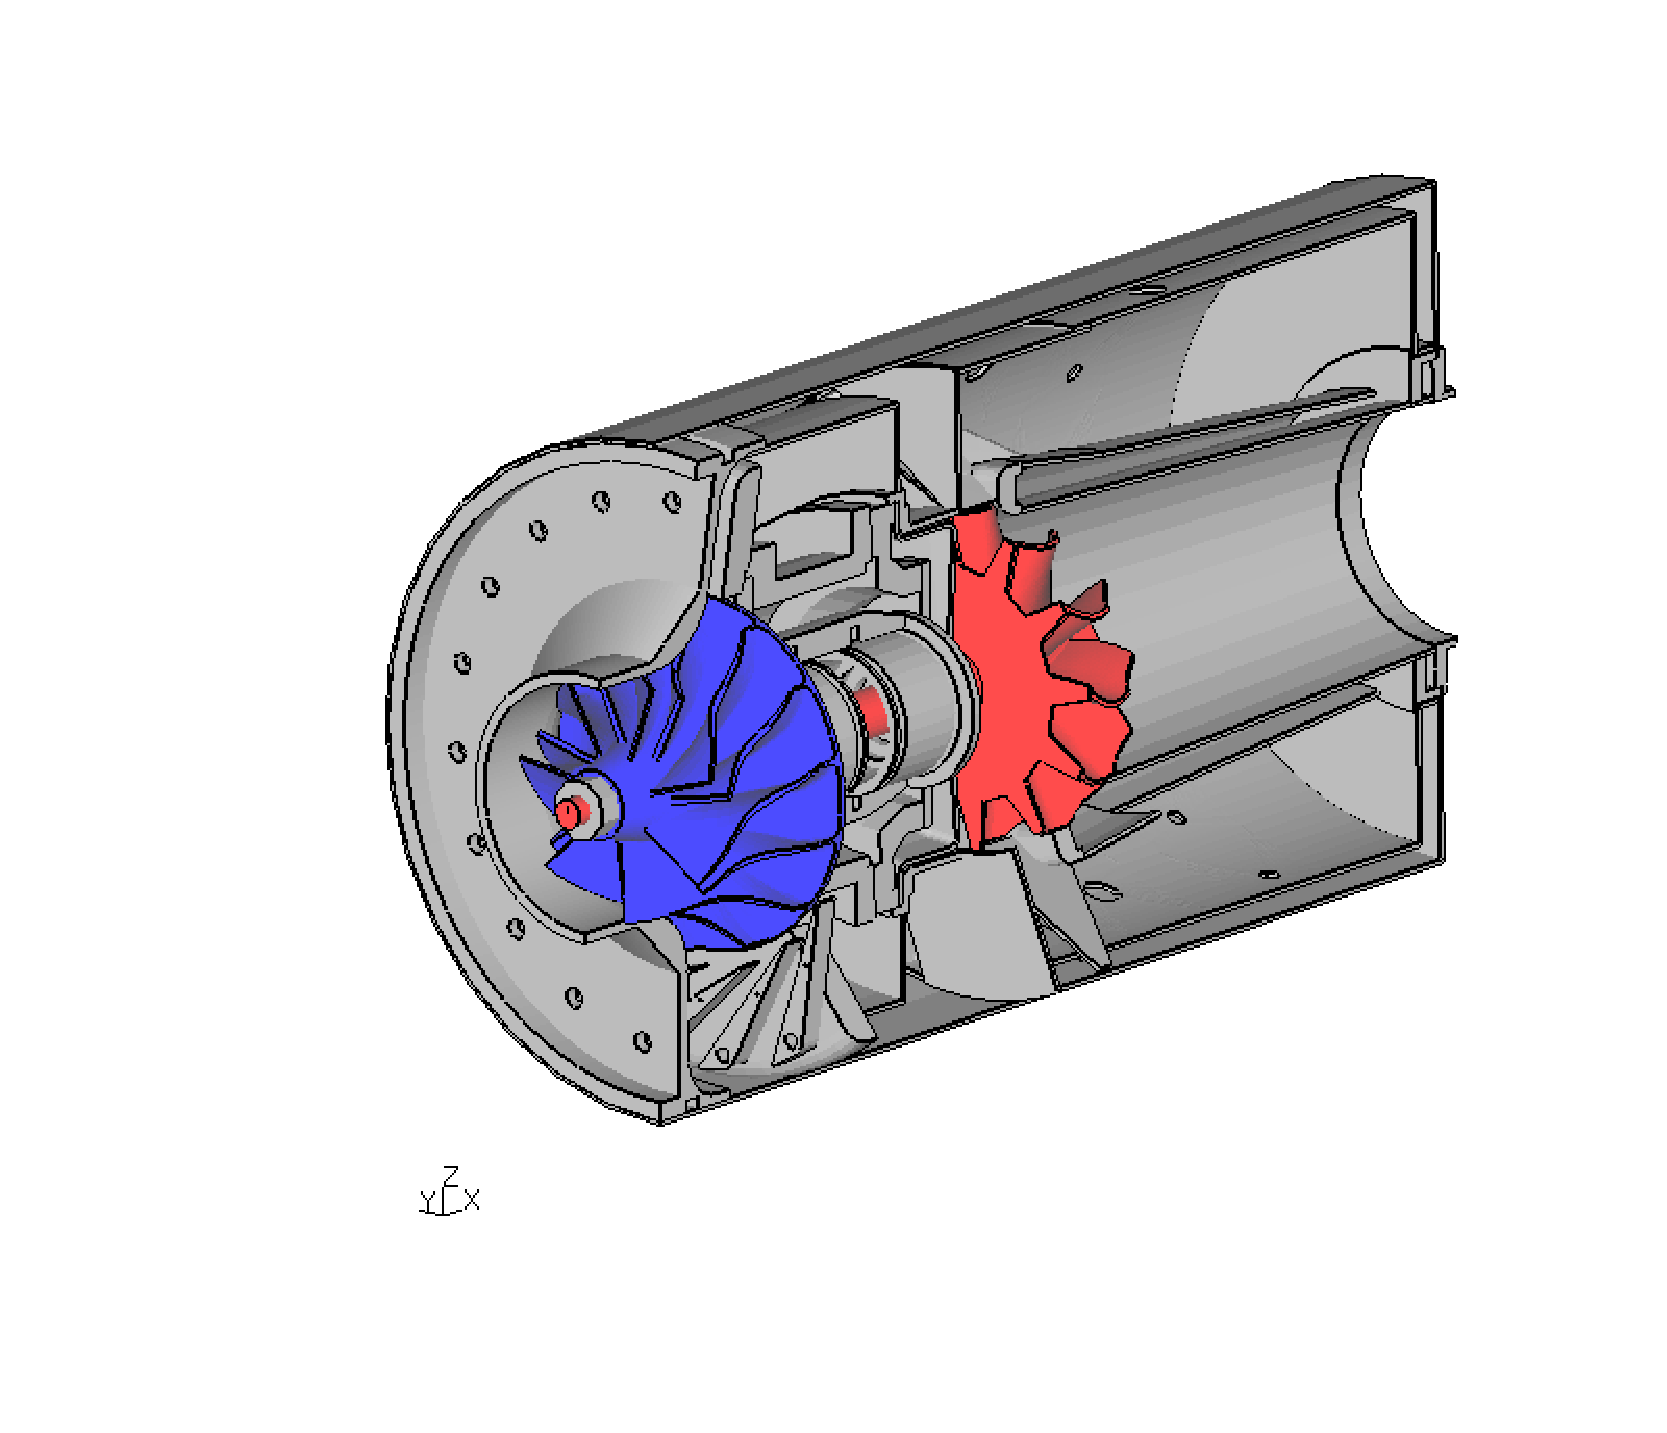
\epsfig{file=jetengine.eps,width=12cm}
\caption{\label{cover} A complex model made from scratch using second order brick elements }
\end{figure}
\newpage


\tableofcontents


\section{Introduction}
 This document is the description of CalculiX GraphiX (cgx). This program is designed to generate and display finite elements (FE) and results coming from CalculiX CrunchiX (ccx). If you have any problems using cgx, this document should solve them. If not, you might send an email to the author \cite{cgx}. The Concept and File Format sections give some background on functionality and mesher capabilities. The Getting Started section describes how to run the verification examples you should have obtained along with the code of the program. You might use this section to check whether you installed CalculiX correctly. Then, a detailed overview is given of the menu and all the available keywords in alphabetical order in the Menu and Commands sections respectively. Finally, the User's Manual ends with the appendix and some references used while writing the code.


\section{Concept}
This program uses the openGL library for visualization and the glut library \cite{glut} for window management and event handling. This results in very high speed if a hardware-accelerated openGL-library is available and still high speed for software-rendering (MesaGL,\cite{mesa}). 

The cgx has pre- and post-processor capabilities. It is able to generate and display beam, shell and brick elements in its linear and quadratic form (fig. \ref{cover}). It can display but not create pentahedra- and tetrahedra-elements. But tets can be generated from within cgx if NETGEN \cite{NETGEN} is installed and the program ng\_vol (part of NETGEN) is accessible (see also ''\htmlref{How to deal with cad-geometry}{How to deal with cad-geometry}'').

The built-in mesher creates a structured mesh based on a description of the geometry. For example, it uses lines for beam elements, surfaces for shell elements and volumes (bodies) for brick elements. The program distinguishes between the mesh and the underlying geometry. Elements are made from faces and faces are made from nodes. If you move a node, the corresponding face(s) and element(s) will follow. The geometry behaves according to the mesh:
Lines are made from points, surfaces are made from lines and bodies are made of surfaces. Surfaces might have 3 to 5 edges and bodies might have 5 to 7 surfaces. As a result, if you modify the position of a point, all related geometry will follow. In other words, if the location of geometric entities is changed, it is necessary to move the points on which the entities rely.  It should be noted that faces exist only on free surfaces of the model.

In addition, entities can be grouped together to make sets. Sets are useful to handle parts of a model. For example, sets can be used to manipulate or display a few entities at a time (see also ''\htmlref{How to define a set of entities}{How to define a set of entities}''). 

Also a simple but powerful entity which can store values (character strings) is available. This values can be derived from previous commands or calculated results by using an internal stack. Simple calculations can be performed. The values can be used to substitute parameters of subsequent commands. The user might measure a distance or calculate a distance and use this value to move a part of the mesh. Together with a 'while' loop, an 'if' case distinguishing command and the possibility to use system calls via the 'sys' command, elaborated batch files can be written.  

After a mesh is created in cgx, it needs written to a file for use with the solver. Likewise, several boundary conditions and loads can be written to files (see also ''\htmlref{How to connect independent meshes}{How to connect independent meshes}'', ''\htmlref{How to define loads and constraints}{How to define loads and constraints}'' and ''\htmlref{send}{send}''). These files need to be added into the control file for later use in ccx. Additional commands, material description and so on must be added with the help of an external editor. 

After the analysis is completed, the results can be visualized by calling the cgx program again in an independent session. The program is primary controlled by the keyboard with individual commands for each function. Only a subset of commands which are most important for post-processing is also available through a pop-up menu. Shaded animations of static and dynamic results, the common color plots and time history plots can be created. Also, a cut through the model can be done which creates a section and it is possible to zoom through the model.

Skilled users might include their own functions. For example someone may need his own functions to manipulate the result-data or he may need an interface to read or write his own results format (see also ''\htmlref{call}{call}'').

Both the pre- and post- processing can be automated in batch-mode (see also ''\htmlref{How to run cgx in batch mode}{How to run cgx in batch mode}'').


\section{\label{File Formats}File Formats}
The following file-formats are available to write(w) and/or read(r) geometric entities:
\begin{itemize}
\item fbd-format(r/w), this format consists of a collection of commands explained in the section ''\htmlref{Commands}{Commands}'' and it is mainly used to store geometrical information like points, lines, surfaces and bodies. All geometry generated by the user is stored in this format. But it can also be used to define a batch job which uses the available commands.
\item step-format(r), reverse engineered based on some cad files. Only points and certain types of lines are supported currently.
\item stl-format(r/w), this format describes a shape using only triangles. This is just for visualization. Meshing takes place in NETGEN \cite{NETGEN} (see the ``read'' command to handle edges generated by NETGEN). 
\end{itemize}
It is hoped by the author that common CAD formats will be supported by stand-alone interfaces which translate into fbd-commands. So far a vda to fbd interface is available. Tet-meshes can be generated based on the resulting fbd-files.\\\\The following file-formats are available to write a mesh and certain boundary-conditions:
\begin{itemize}
\item Abaqus, which is also used by the CalculiX solver ccx.
\item Ansys, most boundary conditions available.
\item Code\_Aster, mesh and sets of nodes and elements are available.
\item Samcef, mesh and sets of nodes and elements are available.
\item dolfyn, a free cfd-code \cite{dolfyn}.
\item duns, a free cfd-code \cite{duns}.
\item isaac, a free cfd-code \cite{isaac}.
\item OpenFOAM, a free cfd-code \cite{OpenFOAM}, only 8-noded brick-elements are supported.
\item Nastran, most boundary conditions available.
\item tochnog, a free fem-code \cite{tochnog}, only 8-noded brick-elements are supported.
\end{itemize}
The following solver-input-file-formats can be read to check the mesh, sets and certain boundary-conditions:
\begin{itemize}
\item Abaqus, this is also used by the CalculiX solver ccx.
\item Netgen, read Netgen native format (.vol)
\end{itemize}
The following file-formats are available to read solver results:
\begin{itemize}
\item frd-format, files of this format are used to read results of previous calculations like displacements and stresses. This format is described in section ''\htmlref{Result Format}{Result Format}.'' It is also used by ccx. 
\item duns, a free cfd-code \cite{duns},
\item isaac, a free cfd-code \cite{isaac},
\item OpenFOAM, a free cfd-code \cite{OpenFOAM}.
\item Nastran, the f06-file can be read (sf. only CHEXA, displacements and stresses).
\end{itemize}
For a more detailed description on how to use cgx to read this formats see ''\htmlref{Program Parameters}{Program Parameters}'' and the program specific ''\htmlref{Tips and Hints}{Tips and Hints}'' sections.  See the ''\htmlref{send}{send}'' command for how to write them from cgx.


\section{\label{Getting Started}Getting Started}
For installation help, see .../Calculix/cgx\_X.X/INSTALL. After the program is installed on your machine, you should check the functionality by running the examples included in the distribution. The examples are located in .../Calculix/cgx\_X.X/examples/. Begin with a result file called result.frd. Just type\\\\  ''cgx result.frd''\\\\and some information is echoed in the xterm and a new window called main window appears on the screen. The name conventions used for the different areas in the main-window are explained in figure \ref{mainwindow}. Now you should move the mouse pointer into the menu-area and press the left mouse-button. Keep it pressed and continue over the menu item ``Dataset'' to ``Disp''. There you release the button. Then press the left button again and continue over ``Dataset'' and ``Entity'' to ``D1''. For background informations look into the subsection ''\htmlref{Datasets}{Datasets}'' and ''\htmlref{Entity}{Entity}'' which explains how to display results. After seeing the values you might play around a bit with the ''\htmlref{Menu}{Menu}''. Before going further, you should read the section ''\htmlref{Input Devices}{Input Devices}''. See also the commands ''\htmlref{steps}{steps}'', ''\htmlref{max}{max}'', ''\htmlref{min}{min}'' (or the combination of max and min ''\htmlref{mm}{mm}'') and ''\htmlref{scal}{scal}'' which might be used to modify the colour representation of the displayed values. For example type ``min 0'' to set the lower value of the colour bar to zero. Now you should study the following interactive commands: Use ''\htmlref{qenq}{qenq}'' to enquire values at nodes. Use ''\htmlref{qtxt}{qtxt}'' to generate node attached texts showing their number and value. Use ''\htmlref{qcut}{qcut}'' to generate a section through the model. And use ''\htmlref{graph}{graph}'' to generate a 2D time history plot (for results with several time-steps) or a 2D plot of values along a sequence of nodes (see ''\htmlref{qseq}{qseq}''). Watch out if you type a command; the cgx window MUST stay active and not the xterm from which the program was started. It is better to stay with the mouse pointer in the cgx window. Next, ''\htmlref{Quit}{Quit}'' the program and type\\\\  ''cgx -b geometry.fbd''\\\\in the xterm. The program starts again but now you see only a wire-frame of the geometry. Move the mouse-pointer into the new window and type ''\htmlref{mesh}{mesh} all''. The mouse-pointer MUST stay in this window during typing and NOT in the xterm from which the program was started. After you see ''ready'' in the parent xterm, the mesh is created. To actually see it, type ''\htmlref{plus}{plus} ea all''. Now you see the mesh in green color. To see the mesh as a wire-frame, choose in the main menu''\htmlref{Viewing}{Viewing}'' and continue to the entry ''\htmlref{Toggle Element Edges}{Toggle Element Edges}'' and then again in ''\htmlref{Viewing}{Viewing}'' choose ''\htmlref{Dots}{Dots}''. To see the mesh illuminated chose in the main menu ''\htmlref{Viewing}{Viewing}'' and continue to the entry ''\htmlref{Show Elements With Light}{Show Elements With Light}''. To see it filled, choose in the main menu ''\htmlref{Viewing}{Viewing}'' and continue to the entity ''\htmlref{Fill}{Fill}''. Most of the time it is sufficient to see the surface elements only. For this purpose, choose in the main menu ''\htmlref{Viewing}{Viewing}'' and continue to the entry ''\htmlref{Toggle Surfaces/Volumes}{Toggle Surfaces/Volumes}''. If you start cgx in the post processor mode, as you did in the first example (cgx result.frd), the surface mode is automatically set. To see the interior of the structure, choose in the main menu ''\htmlref{Viewing}{Viewing}'' and continue to the entity ''\htmlref{Toggle Culling Back/Front}{Toggle Culling Back/Front}''. To save the mesh in the format used by the solver, type ''send all abq''. To store the mesh in the result format type ''send all frd''. 

To create a new model start the cgx by typing\\\\  ''cgx -b file''\\\\where ''file'' will be the name of the new model if you later exit the program with the command ''\htmlref{exit}{exit}''. The way to create a model from scratch is roughly as follows, create
\begin{itemize}
\item points with ''\htmlref{qpnt}{qpnt}'' or ''\htmlref{pnt}{pnt}'',
\item lines with ''\htmlref{qlin}{qlin}'',
\item surfaces with''\htmlref{qsur}{qsur}'',
\item Bodies with ''\htmlref{qbod}{qbod}''.
\end{itemize}
If possible, create higher geometry by sweeping or copying geometry with ''\htmlref{swep}{swep}'' or ''\htmlref{copy}{copy}''. You might move or scale your model with the command ''\htmlref{move}{move}''. The commands require sets to work with. Sets reference entities like bodies or nodes. They are usefull because you can deal with a bunch of entities at once. See the section ''\htmlref{How to define a set of entities}{How to define a set of entities}'' about how to create them.

You can write a file with basic commands like ''pnt'' to create the basis for your construction and read it with the ''\htmlref{read}{read}'' command. Most commands can be used in batch mode. This allows the user to write a command file for repeated actions.

The interactive commands start with the letter 'q'. Please make yourself familiar with all of them before you start to model complex geometry.

After the geometry is created, the divisions of the lines can be changed to control the density of the elements.  Display the lines and their divisions with 
\begin{itemize}
\item ''\htmlref{plot}{plot} ld all''.
\end{itemize}
To change the element division, use 
\begin{itemize}
\item ''\htmlref{qdiv}{qdiv}''.
\end{itemize}
The default division is ''4''. With a division of''4,'' a line will have 6 nodes and will therefore be the edge of two element of the quadratic type. Next, the type of the elements must be defined. This can be done for each of the different sets. A new assignment will replace a previous one. Delete all previous assignments with
\begin{itemize}
\item ''\htmlref{elty}{elty} all''
\end{itemize}
and assign new types with
\begin{itemize}
\item ''\htmlref{elty}{elty} all he20''.
\end{itemize}
If a mesh is already defined type
\begin{itemize}
\item ''\htmlref{del}{del} mesh''
\end{itemize}
and mesh again with
\begin{itemize}
\item ''\htmlref{mesh}{mesh} all''.
\end{itemize}
Then choose the menu entity ''\htmlref{Viewing}{Viewing} - \htmlref{Show Elements With Light}{Show Elements With Light}'' to see the mesh lighted. Lastly, export the mesh in the calculix solver format with
\begin{itemize}
\item ''\htmlref{send}{send} all abq''.
\end{itemize}
With the ''send'' command, it is also possible to write boundary conditions, loads and equations to files. The equations are useful to ''glue'' parts together.\\\\It is advisable to save your work from time to time without exiting the program. This is done with the command
\begin{itemize}
\item ''\htmlref{save}{save}''.
\end{itemize}
You leave the program either with 
\begin{itemize}
\item ''\htmlref{exit}{exit}''
\end{itemize}
or with
\begin{itemize}
\item ''\htmlref{quit}{quit}''.
\end{itemize}
Exit will write all geometry to an fbd-file and if a file of this name exists already then the extension of this file will be renamed from fbd to fbb. ''quit''  closes the program without saving. 

A solver input file can be written with the help of an editor (emacs, nedit etc.). If you write a ccx command file, then include the mesh, the boundary conditions etc. with the ccx command ''*INCLUDE''. After you finished your input-file for the solver (ccx) you might read it by calling the program again with\\\\  ''cgx -c solverfile.inp''\\\\for a final check. All predefined sets are available together with automatically generated sets which store boundaries, equations and more. These sets start with the ''+''-sign. For example the set +bou stores all constrained nodes where the set +bou1, +bou2, +bou3 store the constraints for the individual directions. Further the set +dep and +ind store the dependent and independent nodes involved in equations etc. See which sets are defined with the command
\begin{itemize}
\item ''\htmlref{prnt}{prnt} se''.
\end{itemize}
Each line starts with the set-index, then the set-name followed by the number of all referenced entities. The sets can be specified by index or name. For example if the index of set ''blade'' is ''5'' the following commands are equivalent:
\begin{itemize}
\item ''plot p 5''
\item ''plot p blade''
\end{itemize}
The use of wildcards is possible to search for a certain expression:
\begin{itemize}
\item ''\htmlref{prnt}{prnt} se +*''
\end{itemize}
Now all sets starting with a ``+'' in their names will be listed.

Predefined loads are stored as ''\htmlref{Datasets}{Datasets}'' to be visualized. Sets with the name of the load-type (CLOAD, DLOAD) store the related nodes, faces or elements. Use the command
\begin{itemize}
\item ''\htmlref{plot}{plot}''
\end{itemize}
or
\begin{itemize}
\item ''\htmlref{plus}{plus}''
\end{itemize}
to visualize entities of sets.

Then run the input file with ccx. The result file (.frd) can be visualized with\\\\  ''cgx filename.frd filename.inp''\\\\were the solver input file ''filename.inp'' is optional. With this file, the sets, boundary conditions and loads used in the calculation are available together with the results.\\\\If you have problems doing the above or if you want to learn more and in more detail about the cgx continue with the tutorial \cite{tutorial} and look in the appendix, section \htmlref{Tips and Hints}{Tips and Hints} and \htmlref{Known Problems}{Known Problems}.    


\section{\label{Program Parameters}Program Parameters}
\begin{verbatim}
 usage:
 cgx [-a|-b|-bg|-c|-duns2d|-duns3d|-isaac2d|-isaac3d|-foam|-ng|
      -step|-stl] filename [ccxfile]

  -a        automatic-build-mode, geometry file derived from a 
            cad file is expected
  -b        build-mode, geometry file in fbd-format is expected
  -bg       background, suppress creation of graphic output
            otherwhise as -b, geometry (command) file must be
            provided
  -c        read an solver input file (ccx, Abaqus)              
  -duns2d   read duns result files (2D)                                  
  -duns3d   read duns result files (3D)
  -isaac2d  read isaac result files (2D)                                  
  -isaac3d  read isaac result files (3D)                                  
  -foam     read the OpenFOAM result directory structure
  -f06      read Nastran f06 file.    
  -ng       read Netgen native format (with surface domains)    
  -step     read an ascii-step file (points and lines only)                                  
  -stepsplit read step and write its parts to the filesystem
             in separate directories
  -stl      read an ascii-stl file (triangles)                                  
  [-v]      (default) read a result file in frd-format and
            optional a solver input file (ccx) in addition 
            which provides the sets and loads used in the
            calculation.

 special purpose options:                                               
  -mksets       make node-sets from *DLOAD-values 
                (setname:''_<value>'')
  -read         forces the program to read the complete result-
                file at startup
\end{verbatim}
If no option is provided then a result-file (frd) is assumed, see ''\htmlref{Result Format}{Result Format}''.

A file containing commands or geometric informations is assumed if the option -b is specified. Such a file will be created if you use ''\htmlref{exit}{exit}'' or ''\htmlref{save}{save}'' after you have interactively created geometry. Option -a awaits the same format as option -b but merging, defining of line-divisions and the calculation of the interior of the surfaces is done automatically and the illuminated structure is presented after startup. This should be used if the commandfile was generated by an interface-program which convertes cad-data to cgx-format (for example vda2fbd). With option -a and -b the program will start also if no file is specified. 

An input file for the solver can be read with option -c. Certain key-words are known and the affected nodes or elements are stored in sets. For example the default set(s) +bou(dof) store nodes which are restricted in the corresponding degree of freedom and the set(s) +dep(dof) and +ind(dof) store dependent and independent nodes used in equations.

A special case is OpenFOAM. The results are organized in a directory structure consisting of a case containing time-directories in which the result-files are stored. The user must call cgx using the case-directory (cgx -foam case). The program will then search the time-directories. The time directories must contain a time-file to be recognized. Or in other words each directory in this level containing a time-file is regarded as a result directory.

\section{\label{Input Devices}Input Devices}

\subsection{\label{Mouse}Mouse}
The mouse is used to manipulate the view-point and scaling of the object inside the drawing area (figure \ref{mainwindow}). Rotation of the object is controlled by the left mouse button, zoom in and out by the middle mouse button and translation of the object is controlled by the right mouse button. Inside the menu area, the mouse triggers the \htmlref{main menu}{Menu} with the left button.\\\\In addition the mouse controls the \htmlref{animation}{animation} of nodal values. The animation will stop if the mouse pointer is not in the drawing area but will start again if the pointer enters the drawing area. This can be prevented by pressing the middle mouse button while the mouse pointer is in the menu area.  Pressing the right button will release the next frame. A frozen animation can be released by pressing the middle button. The previous frame can be reloaded by pressing the middle mouse button twice and the right button once (while the mouse is in the menu area).
  
\begin{figure}[h]
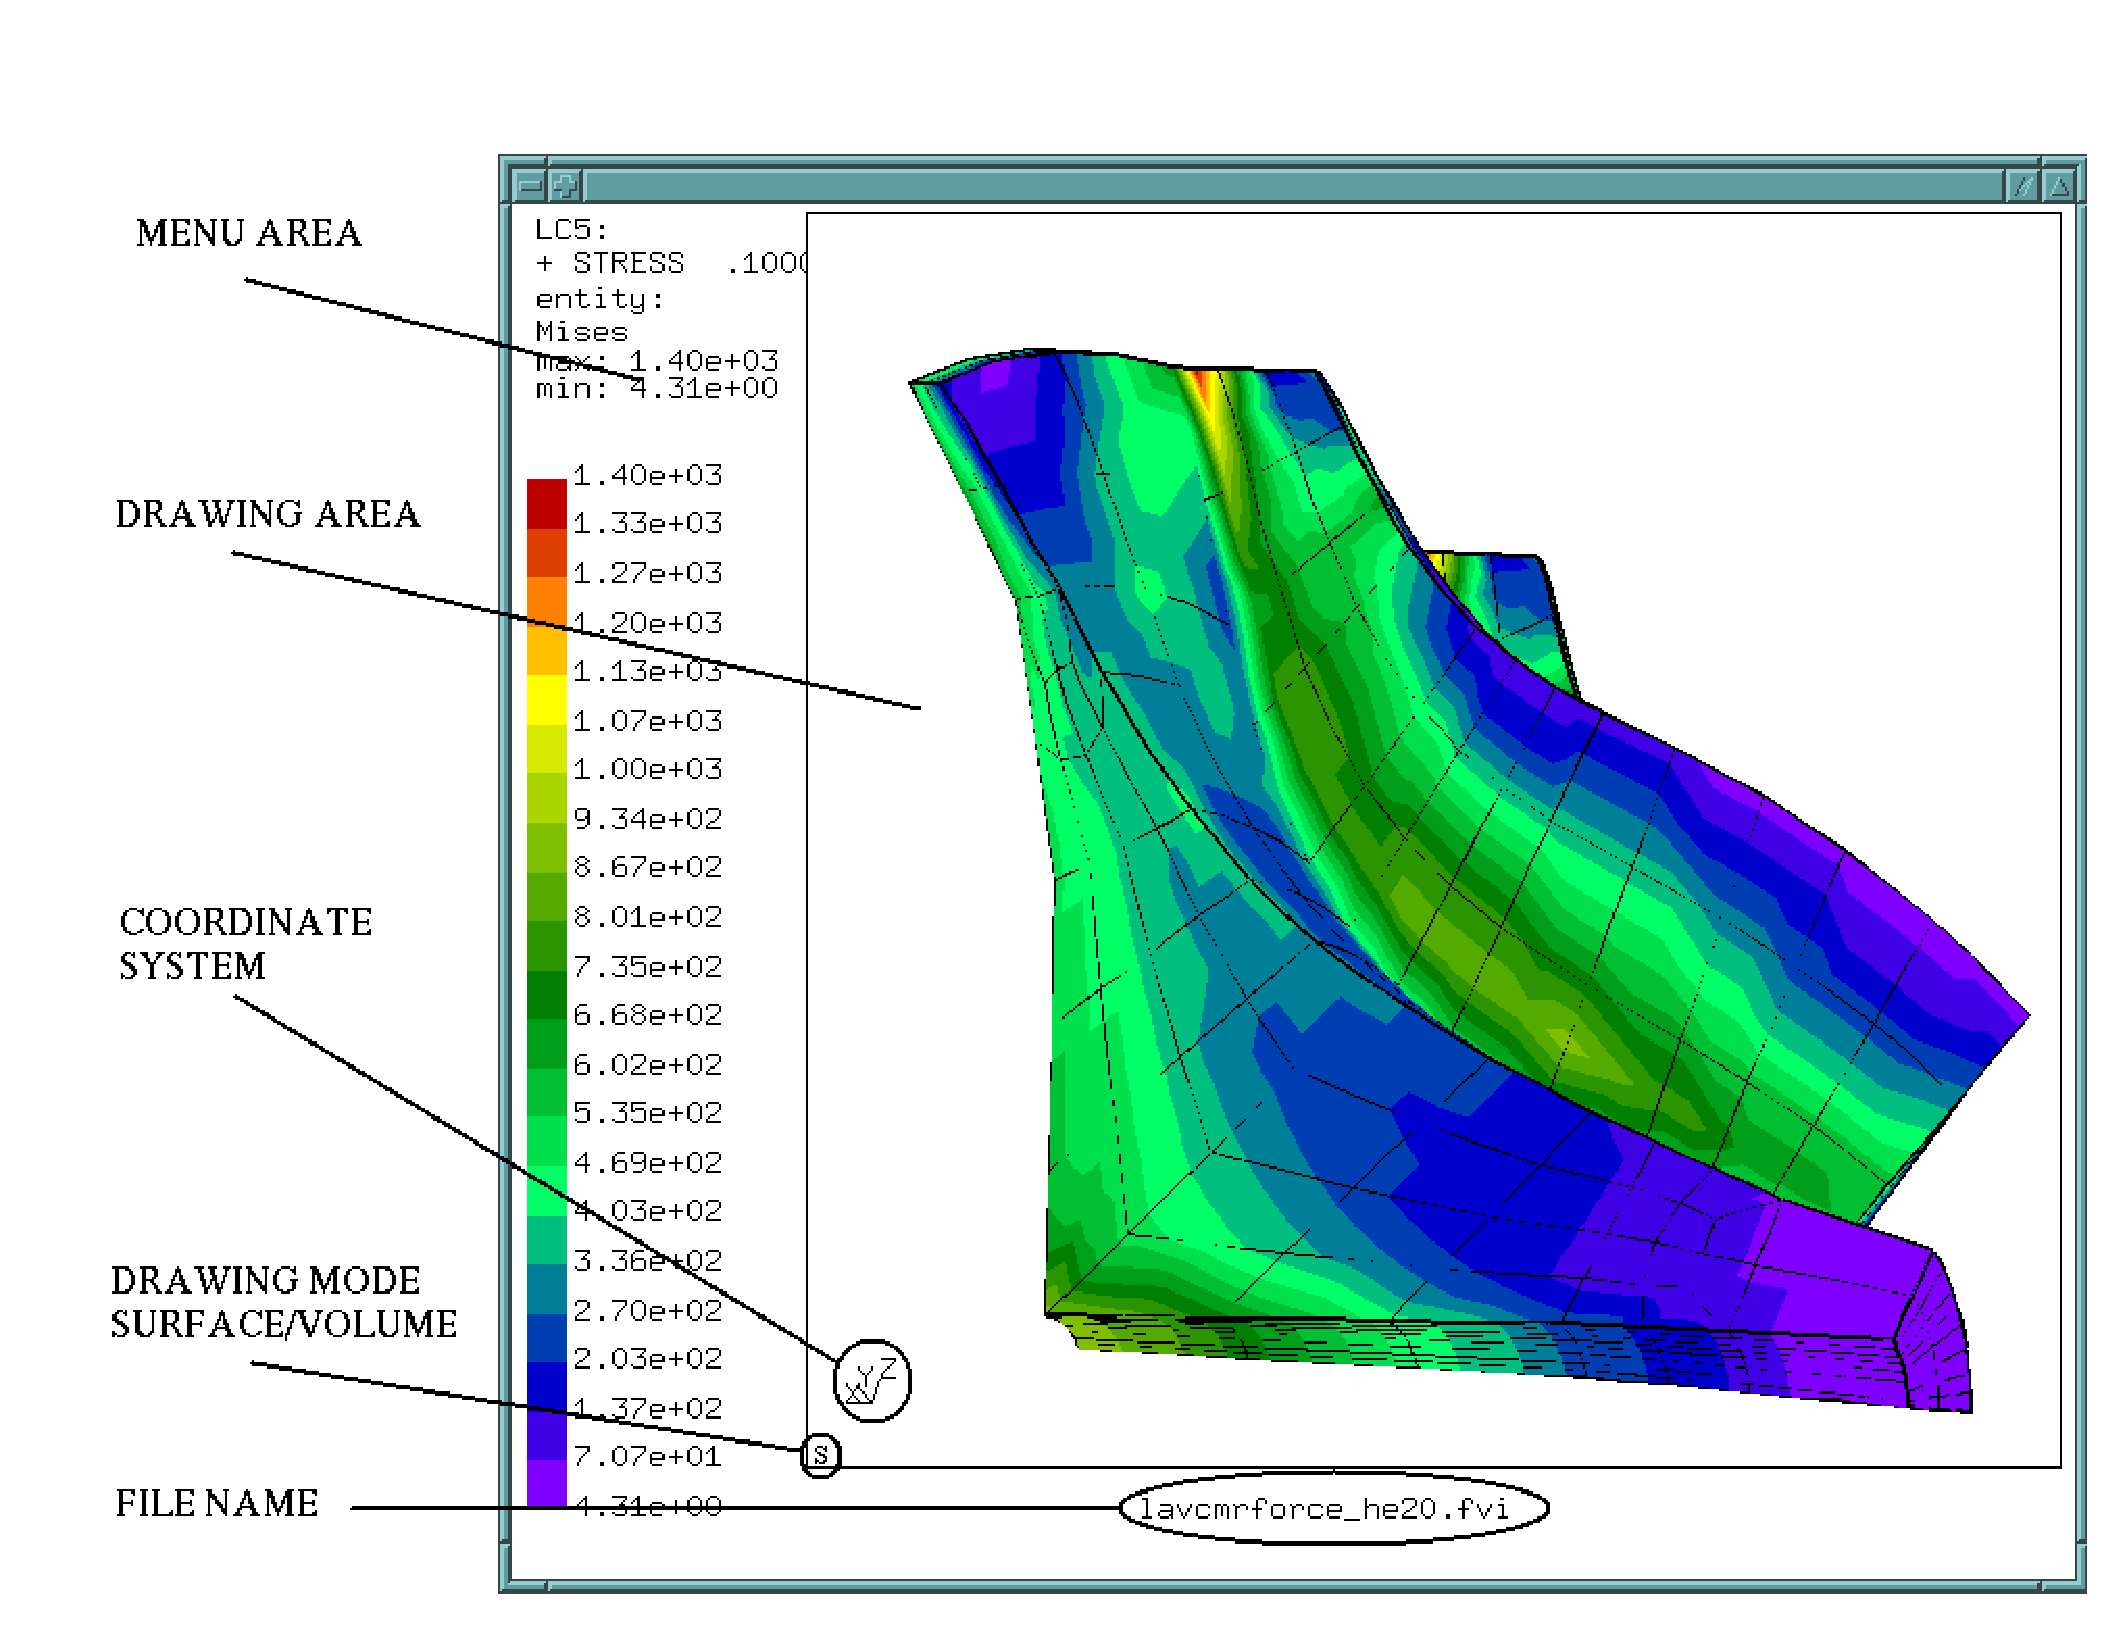
\epsfig{file=mainwindow.eps,width=12cm}
\caption{\label{mainwindow}structure of the main-window}
\end{figure}

\subsection{\label{Keyboard}Keyboard}
The Keyboard is used for command line input and specifying the type of entities when selecting them with the mouse pointer. The command line is preferable in situations where pure mouse operation is not convenient (i.e. to define a certain value) or for batch controlled operations. Therefore most commands are only available over the command line. The stream coming from the keyboard is echoed in the parent-xterm but during typing the mouse pointer must stay inside the main window. Otherwise the commands will not be recognized by the program. 

The following special keys are used:
\begin{verbatim}
Special Keys:
 ARROW_UP:   previous command
 ARROW_DOWN: next command
 PAGE_UP:    entities of previous set (if the last command was
             plot or plus) or the previous Loadcase
 PAGE_DOWN:  entities of next set (if the last command was 
             plot or plus) or the next Loadcase
\end{verbatim}



\section{\label{Menu}Menu}
The main menu pops up when pressing the left mouse-button inside the menu-area (figure \ref{mainmenu}). It should be noted that there are equivalent command-line functions for most of the menu-functions. This can be used for batch-controlled post-processing. Next the entities inside the main menu will be explained:
  
\begin{figure}[h]
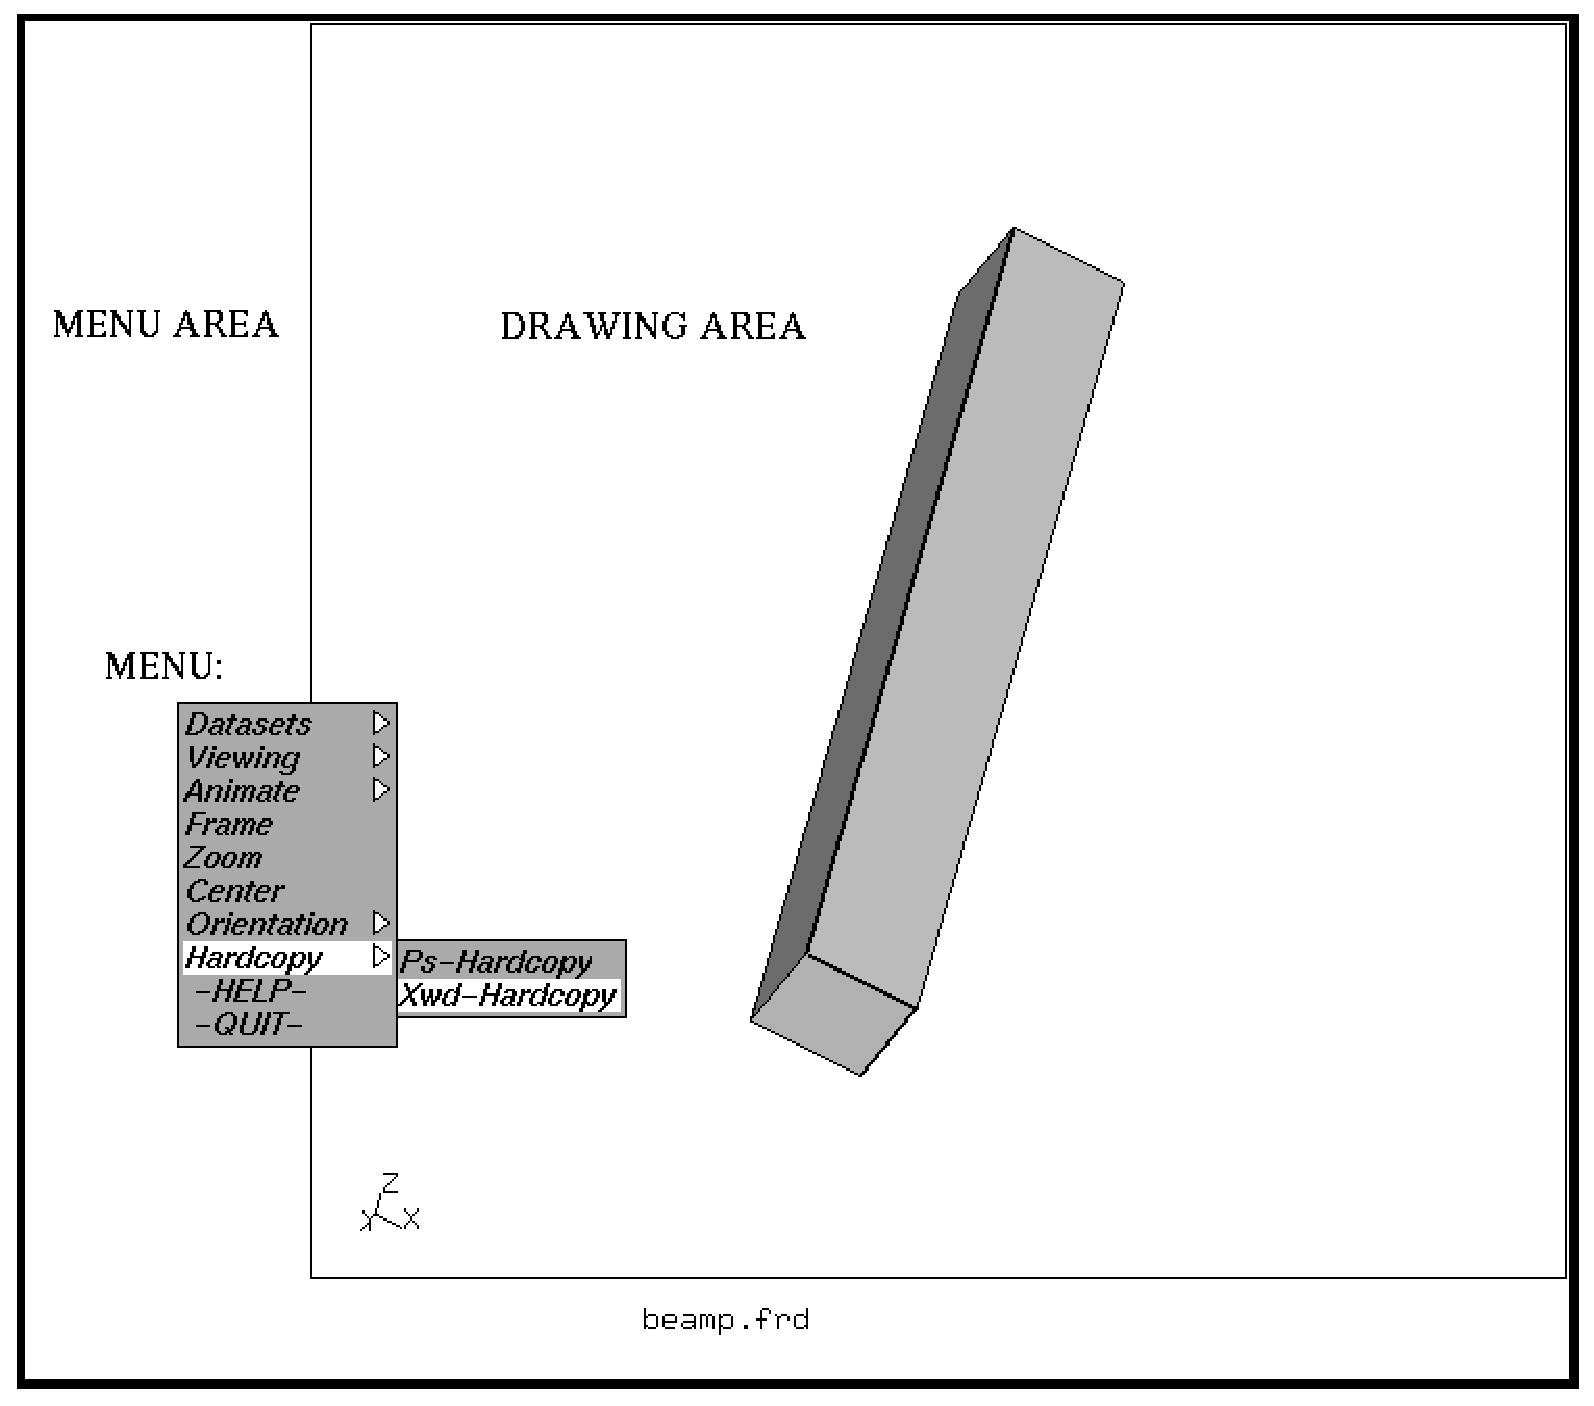
\epsfig{file=mainmenu.eps,width=12cm}
\caption{\label{mainmenu}structure of the main-menu}
\end{figure}


\subsection{\label{Datasets}Datasets}
Datasets are selected with the menu-item ''Dataset''. A dataset is a block of nodal values. These could be displacements due to a linear analysis or for a specific time-step during a nonlinear analysis. It could also contain other values like stresses, strains, temperatures or something else. To select a dataset, make sure that the mouse-pointer is inside the menu area. Then, press the left mouse button and move the mouse-pointer over the menu entry ''Dataset'', then continue to the right. A sub-menu pops up showing all available datasets with a leading number and sometimes followed by a dataset-value (usually time or frequency) and a dataset-description. Move the mouse-pointer over a dataset you are interested in and release the left mouse button. The dataset is now selected. A results ''\htmlref{Entity}{Entity}'' must be chosen to see the values in the drawing-area. This Dataset might also contain automatically calculated values like the v. Mises stress and the maximum principal stress (see \htmlref{Pre-defined Calculations}{Pre-defined Calculations} and \htmlref{Result Format}{Result Format}). See also the command ''\htmlref{ds}{ds}'' to control the functionality with the command-line.

\subsubsection{\label{Entity}Entity}
To view data from the dataset, its also necessary to specify the entity (i.e. dx for a displacement Dataset). It works in the same way as for selecting the dataset but instead of releasing the left mouse button over a Dataset continue to the bottom of the sub-menu to ''Entity.''  Continue from that item to the right and release the mouse button when the pointer is over an entity.  Now the data is displayed in the drawing-area.

\subsection{\label{Viewing}Viewing}
In the following sections, changing properties and styles of the displayed structure are explained. See the command ''\htmlref{view}{view}'' to control the functions with the command-line.

\subsubsection{\label{Show Elements With Light}Show Elements With Light}
This is the default view of the mesh if the program was started in viewing mode. If used, any \htmlref{animation}{animation} will be interrupted and no values are displayed.  

\subsubsection{\label{Show Bad Elements}Show Bad Elements}
This option presents elements which have a negative Jacobian value at least at one integration point. The solver ccx can not deal with those elements. So far, only TET and HEX elements are checked. These elements are stored in the set called -NJBY. See also the command ''\htmlref{eqal}{eqal}''.

\subsubsection{\label{Fill}Fill}
This is the default mode and forces the element faces to be rendered.

\subsubsection{\label{Lines}Lines}
The edges of the element faces are displayed. This is especially useful to see into the structure to find hot spots in the displayed field. With ''\htmlref{Toggle Move-Z/Zoom}{Toggle Move-Z/Zoom}'' and ''\htmlref{qcut}{qcut}'', a more detailed analysis can follow. For very dense meshes switch to ''\htmlref{Dots}{Dots}''.

\subsubsection{\label{Dots}Dots}
The corners of the element faces will be displayed. This is especially useful if values inside the structure need checked.

\subsubsection{\label{Toggle Culling Back/Front}Toggle Culling Back/Front}
This removes the faces of volume elements for all elements or for the surface of the structure, depending on the state of ''\htmlref{Toggle Surfaces/Volumes}{Toggle Surfaces/Volumes}''. With this option, the user can visualize internal structures like cracks or a core of a hollow structure.\\ 
For shell elements, the behavior is different. Initially only the front faces are illuminated and the back faces are dark. This is helpful to determine the orientation of the elements. If you want to see all faces of the shell-elements illuminated regardless of the orientation, then use this option. If you want to change the orientation use the command ''\htmlref{qflp}{qflp}''.

\subsubsection{\label{Toggle Model Edges}Toggle Model Edges}
Per default, all free element edges are shown. The user can remove/show them with this option.

\subsubsection{\label{Toggle Element Edges}Toggle Element Edges}
Per default, just the free element edges are shown. The user might add all edges to the structure with that option.

\subsubsection{\label{Toggle Surfaces/Volumes}Toggle Surfaces/Volumes}
This switches the way each volume elements are displayed. Either all faces of the elements or just the element faces on the surface of the structure are displayed. Depending on the state of ''\htmlref{Toggle Culling Back/Front}{Toggle Culling Back/Front},'' either the faces pointing to the user or the faces pointing away are displayed. The default is just to show the surface pointing to the user. In the lower left corner of the drawing area,(see figure \ref{mainwindow}) a character is printed, indicating the program is in the surface mode ''s'' or in the volume mode ''v''.

\subsubsection{\label{Toggle Move-Z/Zoom}Toggle Move-Z/Zoom}
Instead of zooming in with the help of the middle mouse button, it is also possible to move a clipping plane through the structure to get a view of the inside. The clipping plane is parallel to the screen and will be moved in the direction to and from the user by pressing the middle mouse button and moving the pointer up and down while inside the drawing area. Usually it needs some mouse movements until the clipping plane has reached the structure. Depending on hardware, this functionality could be slow. After zooming in, consider using the ''\htmlref{plot}{plot}'' and ''\htmlref{plus}{plus}'' commands to customize your view.

\subsubsection{\label{Toggle Background Color}Toggle Background Color}
With this option, it is possible to switch between a black and a white background.

\subsubsection{\label{Toggle Vector-Plot}Toggle Vector-Plot}
It is possible to add small ''needles'' to the plot which point with their heads in the direction of the vectors. Only entities which are marked in the database as vectors will be affected. See ''\htmlref{Nodal Results Block}{Nodal Results Block}'' for information on how entities are marked as vectors. Internally calculated vector-results, like the worst principal stress, are marked automatically. If one component or the value of a vector is selected, then the option takes immediate effect.

This option can be used in combination with ''Animate \htmlref{Toggle Dataset Sequence}{Toggle Dataset Sequence}''.\\\\See also the keyboard command ''\htmlref{ds}{ds}'' how to select datasets and entities with the keyboard. In this case, entities which are NOT marked in the dataset as vectors can be displayed with vector-needles. This command line approach with ''ds'' is the only way to display duns-cfd-results with vector-needles. See also the command ''\htmlref{scal}{scal}'' how to manipulate the length of the vectors.  

\subsubsection{\label{Toggle Add-Displacement}Toggle Add-Displacement}
It is possible to display results on the deformed structure. For example, you can display a stress field on the deformed structure. If you know a suitable amplification factor for your displacements then use the ''\htmlref{scal}{scal}'' command to issue this value but this can also be done later. Of course displacements for the Loadcase must be available.


\subsection{\label{animation}Animate}
This option allows the animation of displacements. See also ''\htmlref{anim}{anim}'', ''\htmlref{ds}{ds}'' and ''\htmlref{scal}{scal}'' to use this functionality with the command-line.

It is possible to create this sequence from just one Dataset, see ''\htmlref{Start}{Start}''. This is useful for displaying mode-shapes. See also ''\htmlref{Toggle Dataset Sequence}{Toggle Dataset Sequence}'' to create a sequence from multiple Datasets to visualize dynamic responses.
   
\subsubsection{\label{Start}Start}
Creates a sequence of display-lists to visualize displacements (for example mode-shapes). The program recognizes displacements just by the name of the dataset. This name must start with the letters ''DISP'', otherwise the animation will not start (see ''\htmlref{Nodal Results Block}{Nodal Results Block}'').

\subsubsection{\label{Tune-Value}Tune-Value}
Controls the amplitude of the animation. If ''\htmlref{Toggle Real Displacements}{Toggle Real Displacements}'' was chosen before, the tune-value is equivalent to the amplification of the animation. 

\subsubsection{\label{Steps per Period}Steps per Period}
Determines how many display lists for one period of animation will be used. If ''\htmlref{Toggle Dataset Sequence}{Toggle Dataset Sequence}'' was chosen, then these number of display lists will be interpreted as one period (see \htmlref{Time per Period}{Time per Period}).

\subsubsection{\label{Time per Period}Time per Period}
Determines how many seconds per period. 

\subsubsection{\label{Toggle Real Displacements}Toggle Real Displacements}
To see the correct displacement of each node. The animation can be controlled with the help of the \htmlref{mouse}{Mouse}.

\subsubsection{\label{Toggle Static Model Edges}}
The user can switch on additional undeformed model edges. This is usefull for hardcopies were this edges give a reference to the undeformed shape.

\subsubsection{\label{Toggle Static Element Edges}}
The user can switch on additional undeformed element edges. This is usefull for hardcopies were this edges give a reference to the undeformed shape.

\subsubsection{\label{Toggle Dataset Sequence}Toggle Dataset Sequence}
Creates a sequence of display-lists to visualize values of a sequence of Datasets. The Datasets must use the same type, for example only displacements or only stresses. To activate the animation, after you have selected ``Toggle Dataset Sequence'' choose the first Dataset to be displayed, then the second  and then the last one. Finally choose the entity. The first two datasets define the spacing between the requested datasets and the third-one defines the last dataset to be displayed. The last two selections of datasets can be omitted. Then all datasets which use the same name, starting from the selected one, will be used. The command ''\htmlref{ds}{ds}'' provides the same functionality. 

\subsection{\label{Frame}Frame}
Adjusts the drawing box.

\subsection{\label{Zoom}Zoom}
Use this command to zoom into a rectangular section of the window. After this option is chosen, use the mouse to select the opposite corners of a rectangle.  The display will zoom in on the rectangular area.  Note the rectangle is never shown on the screen (see also ''\htmlref{zoom}{zoom}'').

\subsection{\label{Center}Center}
Used to choose a new center point for the structure. After this option is chosen, pick either a node, a point or the corner of an entity. To easily find the element corners, the function ''\htmlref{Toggle Element Edges}{Toggle Element Edges}'' is triggered automatically (see also ''\htmlref{qcnt}{qcnt}'').

\subsection{\label{Enquire}Enquire}
Used to investigate parameters like the value and the position of a certain node of the model. Pick a node after this option is chosen. To easily find the element corners, the function ''\htmlref{Toggle Element Edges}{Toggle Element Edges}'' is triggered automatically (see also ''\htmlref{qenq}{qenq}'').

\subsection{\label{Cut}Cut}
Used to cut elements and to create a section of new elements and nodes. Either pick three nodes, or, in case a dataset-entity of a vector was already selected, use the menu entry ``vector'' and select just one node. The cutting plane is then determined by the direction of the vector (displacements, worstPS). To easily find the element corners, the function ''\htmlref{Toggle Element Edges}{Toggle Element Edges}'' is triggered automatically (see also ''\htmlref{qcut}{qcut}'' and ''\htmlref{cut}{cut}'')

\subsection{\label{Graph}Graph}
Used to generate a 2D-plot. The option ``Length'' will provide a plot ``value over distance between nodes''. The option ``Datasets'' will provide a plot ``value over Dataset-nr'' and the option ``Time'' will provide ``value over Time''. For the later two options it is necessary to first create an animation with either the command ''\htmlref{ds}{ds}'' or the menu option ''\htmlref{Toggle Dataset Sequence}{Toggle Dataset Sequence}'' (see also ''\htmlref{graph}{graph}'' and ''\htmlref{How to generate a time-history plot}{How to generate a time-history plot}''). To easily find the element corners, the function ''\htmlref{Toggle Element Edges}{Toggle Element Edges}'' is triggered automatically.

\subsection{\label{Orientation}Orientation}
\subsubsection{+x View}
To look along the x-axis.
\subsubsection{-x View}
To look against the x-axis.
\subsubsection{+y View}
To look along the y-axis.
\subsubsection{-y View}
To look against the y-axis.
\subsubsection{+z View}
To look along the z-axis.
\subsubsection{-z View}
To look against the z-axis.

\subsection{\label{Hardcopy}Hardcopy}
To create a hard-copy during animation, it is useful to stop the animation first with the middle mouse button while inside the menu area of the main window and then release one picture after the other with the right button until the desired amplitude or step is reached.
 
\subsubsection{\label{Tga-Hardcopy}Tga-Hardcopy}
To create a window dump in tga format. You might use the program ''convert'' \cite{ImageMagick} to convert this format to others.

\subsubsection{\label{Ps-Hardcopy}Ps-Hardcopy}
To create a window dump in postscript format. The program convert must be installed.

\subsubsection{\label{Gif-Hardcopy}Gif-Hardcopy}
To create a window dump in gif format. The program convert must be installed.

\subsubsection{\label{Png-Hardcopy}Png-Hardcopy}
To create a window dump in png format. The program convert must be installed.

\subsubsection{\label{Start Recording Gif-Movie}Start Recording Gif-Movie}
All frames during an animation are stored. The recording ends after the right mouse button is pressed while in the menu area. Finally all frames are combined in the file ''movie.gif'' which can be displayed with various tools (Firefox \cite{Firefox} or realplay). If the animation is stopped with the middle mouse button while in the menu area, then the movie stops until it is released by pressing the middle mouse button again. See ''\htmlref{movi}{movi}'' for the keyboard options. Further remarks in ''\htmlref{How to change the format of the movie file}{How to change the format of the movie file}''.

\subsection{\label{Help}Help}
Starts the html help and displays this document. It only works if the specified html-viewer is available. The default is Firefox \cite{Firefox} but this can be changed in the ''cgx.h'' file. The search-path for the documentation is also defined in the ''cgx.h'' file. Please make sure that the documentation is in the specified location or change the path in the ''cgx.h'' file and recompile the program after the object-files are deleted.  The default location for the html help is .../CalculiX/cgx\_X.X/doc/cgx and /CalculiX/ccx\_X.X/doc/ccx for cgx and ccx respectively.  The html files must be downloaded directly or compiled from the latex source for this function to work properly. The INSTALL file tells how to compile the latex code to html.  The INSTALL file is located .../CalculiX/cgx\_X.X/ and .../CalculiX/ccx\_X.X/ for cgx and ccx respectively.

\subsection{\label{Quit}Quit}
This terminates the program without a save.

\section{\label{Commands}Commands}
This section is a reference to all commands and their parameters in alphabetic order. If a command is typed the mouse-pointer must be in the main window (figure \ref{mainwindow}). Only the echo of the input stream is visible in the parent xterm. The keywords are not case sensitive but all command parameters are case sensitive. Each reference starts with a short description of the command. The following syntax is used for these descriptions:
\begin{verbatim}
Known commands and syntax:
 '..':   Keyword (either uppercase or lowercase)
 <..>:   Parameter (case-sensitive)
 [..]:   combination of parameters or optional parameter
 (..):   Remark
 |   :   OR
 &   :   AND
 -   :   from-to
 ->  :   command continues in the next line
 RETURN  press the RETURN key 
\end{verbatim}
Entities---with the exception of nodes and elements---are referenced by names which can contain letters and numbers. Usually one to four characters is recommended. If a new entity uses an existing name, the old definition will be overwritten. To overcome this problem, ''alias'' names can be used. An alias name is defined with the \verb_!_ sign in front. An already defined alias name can be referenced by placing the \verb_%_ sign in front. For example:\\\\
LINE \verb_!_L1 \verb_%_P1 \verb_%_P2 \verb_%_SET\\\\will create a line with the alias name L1 and will use the alias names P1 and P2 to define the end-points and uses the set SET to define the point sequence between the end-points. 

\subsection{\label{anim}anim}
\begin{verbatim}
   'anim'  'tune' <value>|'steps' <value>|'time' <value>|->
           'real' ['on'|'off']|'model' ['on'|'off']| ->
           'elem' ['on'|'off']| 'start'
\end{verbatim}
This keyword is used to manipulate the animation of displacements. See also ''\htmlref{ds}{ds}'' and ''\htmlref{scal}{scal}''. The amplification is controlled with ``tune''. ``steps'' defines the number of frames over one periode. ``time'' controlls the duration of one periode. ``real'' switches of the automatic amplification and the real displacements are used instead. In addition the displacements of the negative part of the periode is set to zero. ``model'' switches the static model (undeformed) edges on or of. ``elem'' does this for the element edges. Start the animation with 'start'. The animation stops when using the 'ds' or the 'view' commands with appropriate parameters.

\subsection{\label{area}area}
\begin{verbatim}
   'area' <set> 
\end{verbatim}
This keyword is used to calculate the area and the center of gravity of a set of shell-elements or surfaces of volume-elements. If a 'dataset' is active then an averaged value is calculated.

The command writes to the ''\htmlref{stack}{stack}''.

\subsection{\label{asgn}asgn}
\begin{verbatim}
   'asgn' ['n'|'e'|'p'|'l'|'c'|'s'|'b'|'S'|'L'|'se'|->
          'sh'|'alpha'|'beta'|'nadapt' <value>] | ->
          ['rbe' <value>|'mpc']
\end{verbatim}
This keyword is used to manipulate the behaviour of successive commands.

For example to define the first node or element number which will be used for the next mesh generation. And it is used to redefine the leading character of new entities. The default is D for points p, L for lines l, C for combined lines (lcmb) c, A for surfaces s, B for Bodies b, Q for nurb lines (nurl) L, N for nurb surfaces (nurs) S, A for sets se and H for Shapes sh. For example\\\\asgn p U\\\\will assign the character U as the leading character to all newly created names of points. The automatically created names of geometric entities use 4 characters. If all possible names with the chosen leading letter are in use then the next alphabetical letter is chosen as a leading letter, so after PZZZ follows Q000. If no more letter follow then the amount of letters per name is increased. The maximum number is 8. Each entity has its own name-space. Different entities might use the same name. Remark: Currently nurbs-lines are automatically used to create splines sharing the same name. Nurbs-lines can not be used for other purposes than to be displayed and so far they can not be written to a file.

The command is also used to controll the behaviour of the unstructured triangulator. This unstructured mesher \cite{mesh2d} uses the tree parameters alpha, beta, nadapt for mesh-control. Current default is 0.4 for alpha and beta and 4 for nadapt.

In case Nastran input should be generated it is possible to switch from MPCs to RBEs when using the \htmlref{send}{send} command in combination with the areampc option. The value after ``rbe'' represents the thermal expansion coefficient of this elements:\\\\asgn rbe 0.5e-6\\\\It should be noted that coincident nodes are connected by MPCs either way.
  
\subsection{\label{bia}bia}
\begin{verbatim}
   'bia'  <line> [<bias>]|
   'bia'  <set>  [<bias>]|
                 ['mult'|'div' <factor>]]
\end{verbatim}
This keyword is used to define the bias of a single line or of a set of lines (see \htmlref{qadd}{qadd}). The bias defines the ratio of the length of the first element to the length of the last element. For example,\\\\
bia all 4.5\\\\will force a ratio in which the last element is 4.5 times bigger than the first one. Real numbers are permitted since version 1.5 (see also \htmlref{qbia}{qbia}). To convert from pre 1.5 versions, start the program with the -oldbias option.
  
\subsection{\label{body}body}
\begin{verbatim}
   'body' <name(char<9)>|'!' [<surf1> <surf2>]|
                [<surf1> <surf2> <surf3> <surf4> ->
                <surf5> [<surf6>  <surf6>]]|
                [<set>]
\end{verbatim}
This keyword is used to define or redefine a volume (body). Each body must have five, six or seven surfaces to be mesh-able with hexaeder-elements, otherwise it can only meshed with tets if NETGEN \cite{NETGEN} is installed. However, it is sufficient to specify just the ''top'' and the ''bottom'' surfaces. But if surfaces with 3 or 5 edges are involved then this surfaces have to be the ''top'' and ''bottom'' surfaces. This is also true if surfaces have different line-divisions at opposite edges. The missing surfaces between the ''top'' and ''bottom'' surfaces will be created automatically if they do not already exist (they will always have 4 edges with the same division on opposide edges). But all needed lines must exist. More precisely, only single lines or existing combined lines (\htmlref{lcmb}{lcmb}) can be detected. The user must define the missing surface if just a chain of lines (and no lcmb) is defined between two corner points of the ''top'' and ''bottom'' surfaces before he can successfully use the body command. It is a more convenient way to define a body than the command ``\htmlref{gbod}{gbod}'' but exactly 2 or all surfaces must be specified otherwise the body will not be created (The most convenient way to define bodies is to use the command ``\htmlref{qbod}{qbod}''). 
For example,\\\\body b1 s1 s2\\\\will look for the missing surfaces and if necessary create them if all lines between the corner points of s1 and s2 are defined; the result is the creation of body, b1. Or for example,\\\\body \verb_!_ s1 s2 s3 s4 s5\\\\will create  a body and a new name for it. The new name is triggered by the sign \verb_!_. Here the body is based on 5 surfaces. If the surfaces are not connected, the body is not mesh-able.\\\\In case a body should only be meshable with tets it can be composed of more than 7 surfaces. The definition can be provided by a set of surfaces:\\\\body \verb_!_ surfset\\\\will create  a body based on the surfaces referenced by surfset.

\subsection{\label{break}break}
\begin{verbatim}
   'break'
\end{verbatim}
This keyword is used to end the interpretation of a command file. The program returns to the interactive mode.

\subsection{\label{call}call}
\begin{verbatim}
   'call' <parameters>
\end{verbatim}
This keyword is used to allow the user to control his own functionality in the file ''userFunction.c''. The data-structures for the mesh and datasets are available. The default function calculates the hydrodynamic stresses with the command:\\\\call hydro\\\\See ''\htmlref{User-Functions}{User-Functions}'' for  details. 

\subsection{\label{cntr}cntr}
\begin{verbatim}
   'cntr' <pnt|nod>
\end{verbatim}
Defines a new center-point or -node. This command is intended for batch-mode. See also ''\htmlref{qcnt}{qcnt}'' for the cursor controlled command.


\subsection{\label{comp}comp}
\begin{verbatim}
   'comp' <set|*chars*> 'u'|'d'|'e'
\end{verbatim}
This keyword is used to add all entities to the specified set (see \htmlref{seta}{seta}) which depend on the already included entities (u, up), or to include all entities necessary to describe the already included entities (d, down).\\For example the set ''lines'' stores lines and should also include all dependent points:\\\\comp lines do\\\\Or the set ''lines'' should also include all surfs and bodies which depend on the lines:\\\\comp lines up\\\\In some cases you will need only the end-points of lines. With the option (e, edges)\\\\comp lines e\\\\ only end-points are included in the set. One exception to this logic was introduced for convenience:\\\\comp nodes do\\\\will add all faces described by the nodes in set nodes despite the fact that faces are made from nodes.

Wildcards (*) can be used to search for setnames of a certain expression:\\\\comp E* do\\\\will complete all sets starting with ``E''.

\subsection{\label{copy}copy}
\begin{verbatim}
   'copy' <set> <set> ['scal' <fx> <fy> <fz> <pnt> [a] ]|
                      ['tra' <dx> <dy> <dz> [a]]|
                      ['rot' <p1> <p2> <alfa> [a] ]|
                      ['rot' 'x'|'y'|'z' <alfa> [a] ]|
                      ['rot' <p1> 'x'|'y'|'z' <alfa> [a] ]|
                      ['rad' <p1> <p2> <dr> [a] ]|
                      ['rad' 'x'|'y'|'z'|'p'<PNT> <dr> [a] ]|
                      ['rad' <p1> 'x'|'y'|'z' <dr> [a] ]|
                      ['mir' <P1> <P2> [a] ]| 
                      ['mir' 'x'|'y'|'z' [a] ]| 
                      ['mir' <P1> 'x'|'y'|'z' [a] ] 
\end{verbatim}
This keyword is used to create a copy of a set (see \htmlref{seta}{seta} about sets). Geometry, nodes and elements with their results can be copied. The copy of results is usefull to evaluate additional sectors in case of a cyclic symmetric calculation. The copy is included in the new set. Existing sets are extended by the copied entities if the last parameter ``a'' (append) is provided. Several transformations are available. For example scal creates a scaled copy, the scaling factors fx, fy, fz can be chosen independently,\\\\
Several transformations are available. For example scal creates a scaled copy, the scaling factors fx, fy, fz can be chosen independently,\\\\
copy part1 part2 scal 2 P0 \\
copy part1 part2 scal 1 1 2 P0\\\\
tra will create a copy and will move it away by the vector dx, dy, dz and the optional parameter a will assign the new entities to sets were the mother of each entity is included,\\\\
copy set1 set2 tra 10 20 30 a\\\\
rot will create a copy and will move it around the axis defined by the points p1 and p2 by alfa degrees,\\\\
copy set1 set2 rot p0 px 20.\\\\
or the axis of rotation is given by specifying one of the basis coordinate axes:
copy set1 set2 rot x 20.\\\\
or just one point and a vector of rotation is given by specifying one of the basis coordinate axes:
copy set1 set2 rot p1 x 20.\\\\
rad will create a copy and uses the same transformation options as 'rot' or will create a spherical section if just a single point is defined,\\\\
copy sphere1 sphere2 rad pP0 10.\\\\
mir will create a mirrored copy. The mirror-plane is placed normal to the direction running from P1 to P2 and placed at P2,\\\\
copy section1 section2 mir P1 P2.\\\\
as with 'rot and 'rad' additional transformation options are available:\\\\
copy section1 section2 mir P1 x\\\\
places the mirror at P1 with its normal direction in 'x' direction\\\\
copy section1 section2 mir x\\\\
Places the mirror in the origin with its normal direction in 'x' direction.

\subsection{\label{corrad}corrad}
\begin{verbatim}
   'corrad' <set>
\end{verbatim}
This is a very special command to adjust improperly defined arc-lines, like in fillets. The center points of arc-lines included in the set are moved in a way that each arc-line will run tangentially into a connected straight line. But because the end-points of the arc-lines are not moved only one side of each arc-line will run into a connected line. The other side is not controlled and might end in a sharp corner. Therefore for each arc-line exactly one connected straight line must be included into the set (figure \ref{corradp}).

\begin{figure}[h]
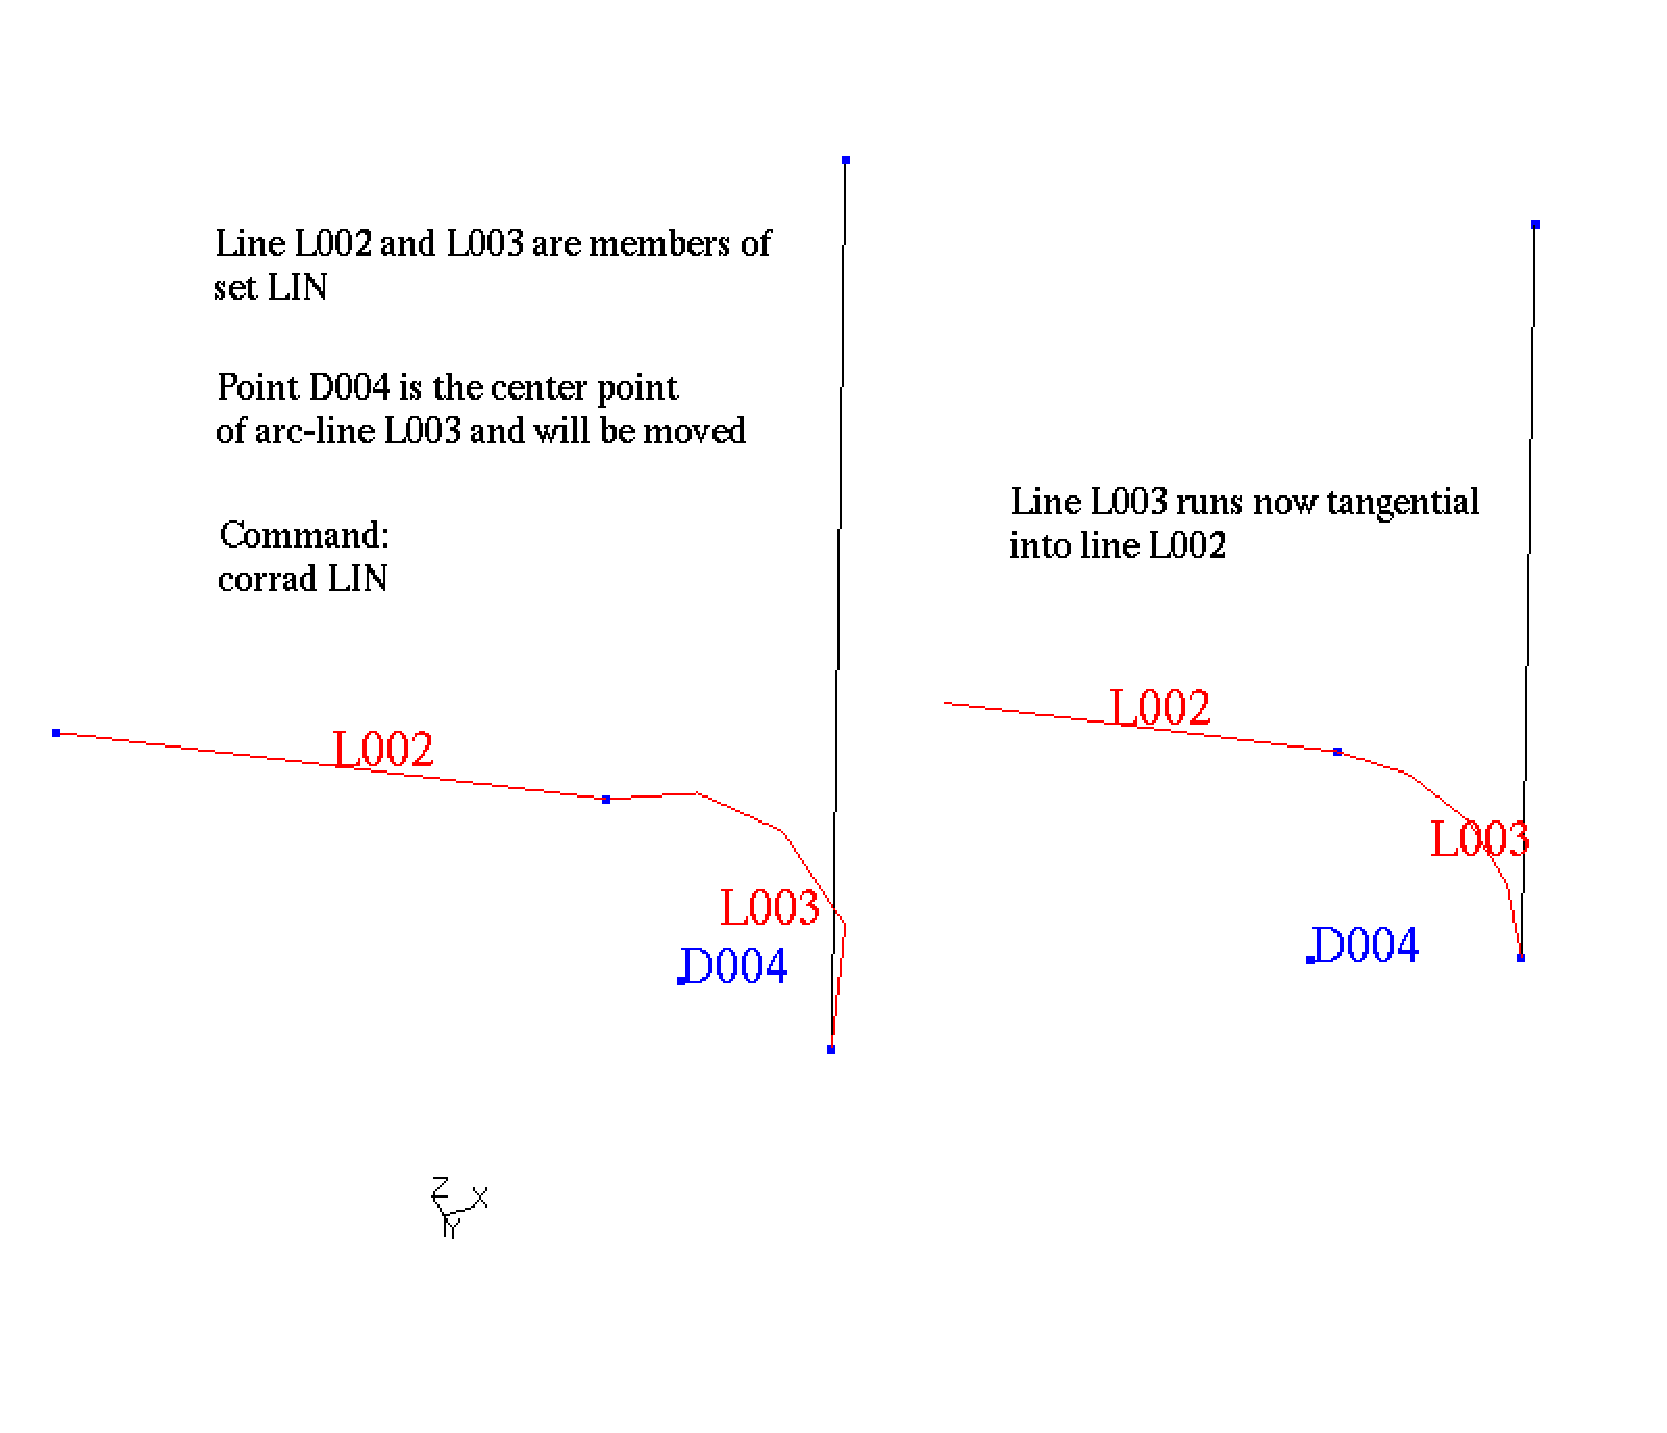
\epsfig{file=corrad.eps,width=9cm}
\caption{\label{corradp} Effect of the corrad command }
\end{figure}

\subsection{\label{csysa}csysa}
\begin{verbatim}
   'csysa' <sysNr> <set>                                                               
\end{verbatim}
Specifies the displacement coordinate system for each node (Nastran only).

\subsection{\label{cut}cut}
\begin{verbatim}
   'cut' <pnt|nod> [<pnt|nod> <pnt|nod>]
\end{verbatim}
This keyword is used to define a cutting plane through elements to visualize internal results. The plane is either defined by three nodes or points, or, in case a dataset-entity of a vector was already selected, by just one node or point. The cutting plane is then determined by the direction of the vector (displacements, worstPS). The menu option ''\htmlref{Show Elements With Light}{Show Elements With Light}'' or the commands ''\htmlref{ucut}{ucut}'', ''\htmlref{view}{view} surf'' or''\htmlref{view}{view} volu'' will display the whole model again and will delete the plane. This command is intended for batch-mode. See ''\htmlref{qcut}{qcut}'' for the cursor controlled command.

\subsection{\label{del}del}
\begin{verbatim}
   'del' ['p'|'l'|'l0'|'c'|'s'|'b'|'t'|'S'|'L'|'se'|'sh' <entity>]|
         ['se0']|
         ['mesh']|
         ['pic'] 
\end{verbatim}
This keyword is used to delete entities, the whole mesh (see also \htmlref{qdel}{qdel}) or a background-picture. For example,\\\\
del se part\\\\
will delete the set ``part'' but all included entities are untouched. The following entities are known:\\\\
Points p, Lines l, Combined Lines c, Surfaces s, Bodies b, Node Texts t, Nurb Surfaces S, Nurb Lines L, Sets se and Shapes sh.\\\\
When an entity is deleted, all dependent higher entities are deleted as well. Special cases are\\\\del l0 set  (l<zero>)\\\\were all lines with zero length in set ''set'' are deleted and\\\\del se0\\\\will delete all empty sets.
If a background-picture was loaded with the ''\htmlref{read}{read}'' command it can be deleted with:\\\\
del pic
\\\\See also ''\htmlref{zap}{zap}'' on how to delete a set with all its referenced entities.

\subsection{\label{dist}dist}
\begin{verbatim}
   'dist' <set> <target-set>|<shpe> ->
              ['tra' <dx> <dy> <dz> <offset>]|
              ['rot' <p1> <p2> <offset>]|
              ['rot' 'x'|'y'|'z' <offset>]|
              ['rad' <p1> <p2> <offset>]|
              ['rad' 'x'|'y'|'z' <offset>]|
              ['nor' <offset> <tol>]   
\end{verbatim}
measures distances between entities of two sets. For example
between points or nodes stored in one set to surfaces or 
shapes stored in a second set. The average-, maximum- and 
minimum distance is determined. The distance is measured
normal-, rotational-, radial or translatoric. The command 
works analogous to the ''\htmlref{proj}{proj}'' command. Please look there for details.

The command writes to the ''\htmlref{stack}{stack}''.
 
\subsection{\label{div}div}
\begin{verbatim}
   'div'  |
          <line> [<division>]|
          <set>  [<division>]|
                 ['mult'|'div' <factor-div> <factor-bias>]|
                 ['auto' <node-dist> <angle> <elem-ratio>] 
\end{verbatim}
This keyword is used to define the division of line(s).  The div keyword also works on a set of lines (see \htmlref{qadd}{qadd}). The division controls the number of nodes created when the geometry is meshed (see \htmlref{elty}{elty} and \htmlref{mesh}{mesh}). For example,\\\\
div all 4\\\\attaches the division of 4 to all lines. With the keyword mult or div in combination with a value, it is possible to multiply or divide already assigned divisions:\\\\
div all mult 2.\\\\Or in case you need a starting-point for the individual divisions you can use the option auto with the optional parameters node-dist and angle. Node-dist is the maximum allowed distance between nodes and angle is the maximum allowed angle defined by three sequential nodes. If one parameter is not fulfilled then the division is halved until the requirements are fulfilled. Default values are defined in the file cgx.h and can be listed with\\\\div\\\\without parameters\\\\
div all auto\\\\uses the defaults. But they can be overruled\\\\div all auto 2. 10. 0.5\\\\will use a maximum element lenght of 2., the angle between successive nodes is less than 10 degree and the minimum element is only half of the maximum-length.
  
\subsection{\label{ds}ds}
\begin{verbatim}
   'ds' <1.Dataset-Nr> [<2.Dataset-Nr>] [<n.Dataset-Nr>] 'a[h]'|'e[h]' ->
   [<entity-nr> (up to 4 times)]|
   ['o' <value> [<entity-nr>]]|
   ['s' <value>] 
\end{verbatim}
This keyword is used to define one or more \htmlref{Datasets}{Datasets} and one or more \htmlref{Entity}{Entity} for display purposes. The Dataset has to be a positive number which has to match the nr in the Dataset-menu or an 'l' (lower case 'L') which is interpreted as the last available Dataset or a negative number. Then it is interpreted as the last ds minus the specified number. For example\\\\
ds 1 e 1\\\\
will display the first entity of the first Dataset.\\\\
ds l e 1\\\\
will display the last Dataset.
To start the animation of the second-to-last Dataset right away:\\\\
ds -1 a\\\\
Or generate an animated fringe plot by adding the desired entity:\\\\
ds -1 a 4\\\\
Sequences can be defined by specifying one to three datasets and by extending the 'e' parameter by an 'h' ('history'):\\\\
ds 2 eh 1\\\\
Here all datasets of the same type as ds 2 are selected. The spacing between datasets of the same type is only evaluated for the first step. A unique step-with is therfore needed.\\\\
ds 2 10 eh 1\\\\
Here the datasets 2, 10 and all successive ones of the same type with a spacing of 8 are selected.\\\\
ds 2 4 10 eh 1\\\\
Here the 1st entity of each second Dataset is selected. The selection starts at the second- and ends at the 10th dataset. If more than one entity is defined then a vector-plot will be displayed. If a 4th entity is defined then this entity will be used for the basic color-plot:\\\\
ds 2 4 10 eh 12 13 14 15\\\\
In case the deformed shape should be shown together with the fringe plot in a sequence of datasets then the 'e' parameter has to be replaced by an 'a' character.\\\\
ds 2 ah 1\\\\ REMARK: So far vector plots can not use the deformed shape. Therefore only one entity is supported.\\\\
In addition, it is possible to scale or offset the entities of the specified datasets:\\\\
ds 1 s 1.2\\\\
will scale all entities of dataset 1 by a factor of 1.2.\\\\
ds 1 o 200.\\\\
will add a value of 200 to all entities of dataset 1.
ds 1 o 200. 2\\\\
will add a value of 200 to the entity 2 of dataset 1.

\subsection{\label{elem}elem}
\begin{verbatim}
   'elem' <nr> <firstNode> .. <lastNode> 'be2'|'be3'|'tr3'|'tr6'|->
   'qu4'|'qu8'|'he8'|'he20'
\end{verbatim}
This keyword is used to define elements based on nodes and its type (see section \htmlref{Element Types}{Element Types} in the appendix for the correct node-order). For example,\\\\
elem 1 1 2 3 4 qu4\\\\creates a shell element with four nodes.

\subsection{\label{else}else}
\begin{verbatim}
  'else'
\end{verbatim}
See the ``\htmlref{if}{if}'' command.

\subsection{\label{endif}endif}
\begin{verbatim}
  'endif'
\end{verbatim}
See the ``\htmlref{if}{if}'' command.

\subsection{\label{endwhile}endwhile}
\begin{verbatim}
  'endwhile'
\end{verbatim}
See the ``\htmlref{while}{while}'' command.

\subsection{\label{elty}elty}
\begin{verbatim}
  'elty' <set> 'be2'|'be2d'|'be3'|->
               'tr3'|'tr3u'|'tr3e'|'tr3s'|'tr3c'->
               'tr6'|'tr6u'|'tr6e'|'tr6s'|'tr6c'|->
               'qu4'|'qu4e'|'qu4s'|'qu4c'|->
               'qu8'|'qu8e'|'qu8s'|'qu8c'|->
               'he8'|'he8f'|'he8i'|'he8r'|->
               'he20'|'he20r'|->
               'te4'|'te10' [<parameter>]
\end{verbatim}
This keyword is used to assign a specific element type to a set of entities (see section \htmlref{Element Types}{Element Types} in the appendix). The element name is composed of the following parts: The leading two letters define the shape (be: beam, tr: triangle, qu: quadrangle, he: hexahedra), then the number of nodes and at last an attribute describing the mathematical formulation or other features (c: axisymmetric, e: plain strain, s: plain stress, u: unstructured mesh, r: reduced integration, i: incompatible modes, f: fluid element for ccx). If the element type is omitted, the assignment is deleted. If all parameters are omitted, the actual assignments are posted:\\\\
elty\\\\
will print only the sets with assigned elements. Multiple definitions are possible. For example,\\\\
elty all\\\\
deletes all element definitions. If the geometry was already meshed, the mesh will NOT be deleted. If the \htmlref{mesh}{mesh} command is executed again after new assignments has taken place, additional elements will be created.\\\\
elty all he20\\\\
assigns 20 node brick-elements to all bodies in the set all.\\\\
elty part1 he8\\\\
redefines that definition for all bodies in the set part1.\\\\
elty part2 tr6u\\\\
assigns 6 node unstructured triangle elements to all surfaces in set part2.\\\\
elty part2 tr6u 0.5\\\\
will do the same but specifies a mesh refinement factor of 0.5 (\verb_>_1: coarser than the average boundary spacing, \verb_<_1: denser ). Be aware that specialiced unstructured meshes must be created by using two times the elty command:\\\\
elty part2 tr6u\\
mesh all\\
elty part2 tr6c\\\\
creates an axisymmetric unstructured mesh.\\\\
elty part3 te10\\\\
assigns 10 node elements to all bodies in set part3. But this works only if NETGEN \cite{NETGEN} is installed and the program ng\_vol is accessible.\\\\
elty part3 te10 3.5\\\\
will do the same but specifies a target size for the elements. In this case the modified program ng\_vol from the cgx-distribution must be available. Replace the original ng\_vol in the NETGEN package and build it again.

\subsection{\label{enq}enq}
\begin{verbatim}
   'enq' <set> <set> ['set' <setname> ]| -> 
            ['rec' <x-value>|'_' <y-value>|'_' <z-value>|'_' ]| ->
            ['cyl' 'x'|'y'|'z' <r-value>|'_' <axis-value>|'_' ] -> 
             <tol> 'i'|'a'|'h'|'l' [<value>]
\end{verbatim}
This command is used to locate entities from a certain set (first provided set) and stores them in the second set. The following entities are handled: nodes, points, lines, surfaces. But surfaces can only be identified if the command ``\htmlref{rep}{rep} \verb_<_setname\verb_>_'' was issued before. In case of nodes with related values (results) it will also determine the highes or lowest value in the specified range, or, all nodes above or below a certain value. The coordinates might be taken from one node or point in a given 3rd set or given in cartesian coordinates (option rec) or cylindrical coordinates (option cyl). Some coordinates might be omitted to specify an infinite range. The '\_' key has to be used in this case. The mode is defined by the keys 'i' individual, 'a' all, 'h' high, 'l' low, were h and l will search the highest or lowest value in range. This value will also be written to a file for automatic processing purposes. For example\\\\
enq all newset rec 10. \_ 100. 0.1 i\\\\
will search for entities in set 'all' at the given location x:10. y:\_(infinite range, triggered by the '\_' key) z:100. with a tolerance of 0.1 and only the closest entity of all kinds of entities are stored in set 'newset', triggered by the 'i' key. With the 'a' key all in range would be stored. The key 'h' or 'l' would trigger a search for the highest or lowest value in the specified range. 

In combination with a certain value\\\\
enq all newset rec 10. \_ 100. 0.1 h 1013.\\\\all nodes with a value above ``1013.'' would be stored in set ``newset''. The command \\\\
enq domain1 newset cyl x 100. 10. 0.1 a\\\\
will search for entities in set 'domain1' at radius:100. around x at x:10. with a tolerance of 0.1. All entities in range are stored in set 'newset'.

The following example illustrates the use of ``enq'' to find the highest value close to a location given by a node-number: 
\begin{verbatim}
# activate dataset 3 with entity 7:
ds 3 e 7
# read a file with one node to define a set:
read pos1.frd pos1
# search the highest value around a radius of 1:
enq all t set pos1 1. h
# move the file with the search result to a meaningfull name:
sys mv enq_lc3_e7_1.out pos1.out
\end{verbatim}
The command writes to the ''\htmlref{stack}{stack}''.


\subsection{\label{eqal}eqal}
\begin{verbatim}
   'eqal' 'jbir'|'aspr'|'mca' <value>
\end{verbatim}
The keyword without parameters lists the current element quality thresholds (0==off):
\begin{itemize}
\item JBIR: The maximum ratio of jacobian determinants xsj between all gaus-points. Were xsj = Vworldcoordinates \verb_/_ Velementcoordinates and jbir = xsj-max \verb_/_ xsj-min. 
\item ASPR: Element aspect ratio between all element sides.
\item MCA: Maximum corner angle between all element sides.
\end{itemize}
With parameter ``value'' sets the value of the threshold.

\subsection{\label{exit}exit}
\begin{verbatim}
   'exit' 
\end{verbatim}
This command terminates the program and saves the geometry (if any) to a file named as the input file but with the extension .fbd. If a file with that name exists already, then this file will be saved with the new file extension .fbb as a backup (see also \htmlref{save}{save}).

\subsection{\label{flip}flip}
\begin{verbatim}
   'flip' <setname>|<surf> ['auto']
\end{verbatim}
This command changes the orientation of a set of surfaces or a single surface. In case of a single surface with the parameter ``auto'' all surfaces will be flipped in a way that they share a common direction (in or out of a volume). See also \htmlref{qflp}{qflp}. 

\subsection{\label{flpc}flpc}
\begin{verbatim}
   'flpc'
\end{verbatim}
This command changes the colour of the scale. Initialy the default is red for high values and blue for low values. The command will invert the current state.

\subsection{\label{font}font}
\begin{verbatim}
   'font' 'd'|'l' <value(1-6)>
\end{verbatim}
This command changes the drawing-font. Six fonts of different heigh are available:
\\\\font d 6\\\\selects the highest font for the drawing area were\\\\font l 1\\\\selects the smallest one for the legend. The default is selected if no number is specified:\\\\font d or font l

\subsection{\label{frame}frame}
\begin{verbatim}
   'frame' 
\end{verbatim}
This command fits the model into the drawing area. 

\subsection{\label{gbod}gbod}
\begin{verbatim}
   'gbod' <name(char<9)>|'!' 'NORM' '+|-' <surf> '+|-' <surf> ->
   .. ( 5-7 surfaces )
\end{verbatim}
This keyword is used to define or redefine a body in the most basic way (see also ``\htmlref{qbod}{qbod}''). Each body must have five to seven surfaces to be mesh-able. However, the number of recommended surfaces is six. The first two surfaces should be the ''top'' and the ''bottom'' surfaces. For example,\\\\gbod B001 NORM - S001 + S002 - S005 - S004 - S003 - S006\\\\will create a body B001. The keyword ''NORM'' is a necessary placeholder for future functionallity but has no actual meaning. Next, follow the surfaces with a sign ''+'' or ''-'' in front that indicates the orientation of each surface. These signs will be corrected automatically if necessary. If the an automatically generated name is desired, then type ''\verb_!_'' instead of a name.

\subsection{\label{gonly}gonly}
\begin{verbatim}
   'gonly' 'on'|'off' 
\end{verbatim}
This keyword is used to erase the contents of the menu area. Sometimes this is useful for hardcopies.

\subsection{\label{graph}graph}
\begin{verbatim}
   'graph'  [<amplitude|*chars*> 'amp' ['l']]|
            [<material|*chars*> 'mat' ['l']]|
            [<set|seq> 'length' ['+'|'-']]| 
            [<set>|'-p' 'nr'|'time'|'descr'|<parameter-name> ->
              [<Dataset-name> <entity-name>|<parameter-name> ] ->
                [<first-Dataset-Nr> <last-Dataset-Nr>]  ]
\end{verbatim}
This keyword is used to create time history plots of nodal values. The values of the pre-selected nodes stored in the referenced set will be written to a file called ''graph.out''. A gnuplot command file will be written called ''graph.gnu'' and executed. The resulting file ''graph.ps'' will be automatically displayed with the postscript viewer. The default is ''ghostview'' but this can be changed in the ''cgx.h'' file before the program is build. See also ``\htmlref{How to generate a time-history plot}{How to generate a time-history plot}'' for further details.

A set with the nodes of interest must be created (usually with ``\htmlref{qadd}{qadd}'') before a graph can be drawn. If the parameter l (length) is used to plot values along the length of a set of nodes then this set should be of the sequence type (usually created with ``\htmlref{qseq}{qseq}''):\\\\graph seq length\\\\The length is calculated as the sum of the distances between successive nodes. Un-ordered sets (as created with ``qadd'') will be ordered in a way that the positive direction points away from the origin of the coordinate system. The direction can be chosen with a '+' or '-' sign following the 'length' parameter ('+' is default).

Instead using existing nodes it is possible to use a line or a combined line ``\htmlref{lcmb}{lcmb}'' as a method to generate new locations for data-points. The current displayed results will be automatically mapped to this locations and shown in a 2D graph over the length of the line:\\\\graph lineset length +\\\\The set lineset stores a line. Since a '+' was given the graph starts at the beginning of the line. With a '-' it would start at the end of the line. 

Since version 1.8, there are two ways of operation. One way is to specify the Datasets and the entity as parameters of the command\\\\graph set time DISP D1\\\\which will display the displacement D1 of nodes in ''set'' vs. the dataset-time of all ''DISP'' Datasets. The first and the last dataset can be specified optionally.

For the traditional way, a sequence of datasets must have been selected (see  \htmlref{Toggle Dataset Sequence}{Toggle Dataset Sequence}). After the selection of the datasets, an \htmlref{Entity}{Entity} must be specified. Then, the user could use the graph command to generate the history-plot of this pre-defined sequence. The command\\\\graph set nr\\\\will display the values on the node-positions vs. the dataset-numbers. The command\\\\graph set time\\\\will display the values on the node-positions vs. the dataset-values (usually time or frequency, see \htmlref{Nodal Results Block}{Nodal Results Block}, parameter ``VALUE'')) and the command\\\\graph set descr\\\\will display the values on the node-positions vs. the dataset-description (only makes sense if the description is a numerical value. See \htmlref{Nodal Results Block}{Nodal Results Block}), parameter ``TEXT'', for the location of this data in the frd-file.\\\\In addition, a second data-file is written ''graph.out2'' which stores the node-number and the node-coordinates and all values at this node-position for all datasets. This file can be used to display values over node-positions, etc. It is up to the user to generate a suitable plot out of this data.\\\\The ''graph'' files can be edited and combined. For example to plot one type of value vs. another type of value.\\\\

If an ccx- or Abaqus-input-file was read then it is also possible to create time history plots of the amplitudes (*AMPLITUDE in ccx) or the material-properties can be displayed (*MATERIAL in ccx):\\\\graph amplitude-name amp\\\\graph material-name mat\\\\Wildcards (*) can be used to search for amplitudes or materials of a certain expression. They are listed with all values if the parameter ``l'' follows after ``amp'' or ``mat'':\\\\graph *N* amp l\\\\lists all amplitudes which contain the 'N'-key in its name with all values.

The parameters related to datasets can also be displayed with the graph command:\\\\graph -p time DISP HID\\\\This command plots the nodal-diameters used in a cyclic symmetry calculation over the dataset-value. Only few parameters are written from ccx in frd-format. Other applications might define its own parameters in frd-format (see \htmlref{Parameter Header Record}{Parameter Header Record} for the format of a parameter record).  

\subsection{\label{grps}grps}
\begin{verbatim}
   'grps'
\end{verbatim}
The result format allows to assign elements to a group. One element can only belong to one group. This command creates sets and stores all elements of a certain group in a certain set called ``+grp[nr]''. See ``\htmlref{Element Definition Block}{Element Definition Block}'' how this applies to the result format (frd).

\subsection{\label{gsur}gsur}
\begin{verbatim}
   'gsur' <name(char<9)>|'!' '+|-' 'BLEND|<nurbs>|<shape>' ->
          '+|-' <line|lcmb> '+|-' <line|lcmb> .. (3-5 times)
\end{verbatim}
This keyword is used to define or redefine a surface in the most basic way (see also \htmlref{qsur}{qsur}). Each surface which is intended for a regular mesh must have three to five edges which might consist of a single line or a combined line (see \htmlref{lcmb}{lcmb}) to be mesh-able. However, the recommend amount of edges is four. For example,\\\\gsur S004 + BLEND  - L002 + L00E + L006 - L00C\\\\will create the surface S004 with a mathematically positive orientation indicated by the ''+'' sign after the surface name. The keyword ''BLEND'' indicates that the interior of the surface will be defined according to Coons \cite{Coons} or a NURBS surface (\htmlref{nurs}{nurs}) or shape (\htmlref{shpe}{shpe}) is referenced. It should be mentioned that only nurbs or shape related surfaces can be meshed with unstructured triangles. Use a  ''+'' or ''-'' in front of the lines or lcmbs to indicate the orientation. These signs will be corrected automatically if necessary. If the surface is intended for an unstructured mesh it is not necessary to care about the correct orientation of the lines and the number of edges is not limmited. If automatic name generation is desired, then use ''\verb_!_'' instead of a name.

\subsection{\label{gtol}gtol}
\begin{verbatim}
   'gtol' [<geometric-tol>]
\end{verbatim}
This keyword is used to enquire the default geometric tolerance:\\\\
gtol\\\\
Or it is used to set the default geometric tolerance:\\\\
gtol value\\\\
The \htmlref{merg}{merg} command will recognize points or nodes as equally located when the distance between them is less than gtol.

The command writes to the ''\htmlref{stack}{stack}''.

\subsection{\label{hcpy}hcpy}
\begin{verbatim}
   'hcpy' ['ps'|'xwd'|'gif'|'png']|[make [ls]]|[clean] (def:xwd)
\end{verbatim}
This keyword creates a hardcopy in one of the above formats. Default is xwd. Use the program ''convert'' to convert to other formats if needed.\\\\hcpy ps\\\\will create a ps file.\\\\hcpy make ls\\\\will bundle all ps files created in one file using the landscape (ls) format. The ls parameter may be omitted. A maximum of six pictures is placed on each page.\\\\hcpy clean\\\\will remove all ''hcpy'' files. See also the commands ''\htmlref{text}{text}'', ''\htmlref{rot}{rot}'', ''\htmlref{ds}{ds}'', ''\htmlref{max}{max}'', and ''\htmlref{min}{min}'' which might be used in hcpy batch files. These commands should be used in the shown order before using the ''hcpy'' command.

\subsection{\label{help}help}
\begin{verbatim}
   'help'
\end{verbatim}
This keyword prints a short overview of all commands.

\subsection{\label{if}if}
\begin{verbatim}
   'if' <value> 'eq'|'ne'|'=='|'!='|'<'|'>' <value>
\end{verbatim}
This keyword is used to compare two values. If the compare is True the following commands are executed. If the compare is False the code after 'else' is executed. Normal operation continues after 'endif':
\\\\if arg1 == arg2\\\\will skip successive commands when the nummerical value stored in 'arg1' is not equal to the nummerical value stored in value 'arg2'. The values are locally converted to 'float' format for the nummerical comparison. The 'eq' and 'ne' compare strings and should not be used for nummerical values since no conversion to a common format is done. Two strings are equal if they have the same length and all characters are equal.

See also ``\htmlref{while}{while}'', ``\htmlref{valu}{valu}'', ``\htmlref{stack}{stack}'' and ``\htmlref{How to run cgx in batch mode}{How to run cgx in batch mode}''.

\subsection{\label{lcmb}lcmb}
\begin{verbatim}
   'lcmb' <name(char<9)>|'!' ['+|-' <line> '+|-' <line> '+|-' ->
   <line>..(up to 14 lines)]|
                          ['ADD' '+|-' <line> '+|-' <line> ->
   '+|-' <line>..(up to 14 lines)]
\end{verbatim}
This keyword is used to define, extend or redefine a combined line (lcmb). Combined lines are necessary if the edge of a surface should be made of more than one line. Usually the user does not create lcmb's directly. They are created automatically during the process of defining a surface with the command \htmlref{qsur}{qsur}. There is no limitation to the number of lines in a combined line. However with one command, not more than 14 lines can be specified at a time. To specify more than that or to extend an existing lcmb a modify command has to follow. For example,\\\\lcmb U260 + U249 - U248 - U247 - U243 - U237 - U236 - U231 - U219 \\\\defines the lcmb U260 with 8 lines and their orientation in the lcmb. The following command\\\\lcmb U260 ADD - U218 - U217\\\\extends the lcmb U260 by two additional lines.

\subsection{\label{length}length}
\begin{verbatim}
    'length' <set>
\end{verbatim}
This keyword is used to calculate the length of all lines stored in a set.

The command writes to the ''\htmlref{stack}{stack}''.

\subsection{\label{line}line}
\begin{verbatim}
   'line' <name(char<9)>|'!' <p1> <p2> <cp|seq> <div> [<bias>] 
\end{verbatim}
This keyword is used to define or redefine a line. A line depends on points. A line can only be defined if the necessary points are already defined. There are three different types of lines available. The straight line\\\\
line l1 p1 p2 4\\\\
is defined by: its name l1 (the name could have up to 8 characters), by the points p1 and p2 and optionally by the division. The arc\\\\
line \verb_!_ p1 p2 cp 4\\\\
needs a center point cp. The radius changes linear from p1 to p2 if the center-point cp is excentric. The name is chosen automatically (triggered by the character \verb_!_). The spline\\\\
line l1 p1 p2 seq 4\\\\
needs a so called sequential-set, seq (use the command ``\htmlref{seqa}{seqa}'' or ``\htmlref{qseq}{qseq}'' to define such a set). This set seq stores the spline points between the end-points in the right order. The spline function is described in \cite{spline}. Usually, a line is defined interactively with ``\htmlref{qlin}{qlin}''. 

\subsection{\label{lnor}lnor}
\begin{verbatim}
   'lnor' <name|!> <p1> <p2> <p3> <length> 
\end{verbatim}
A new line normal to a plane defined by three points and a length is created. It starts at the last point.

\subsection{\label{mata}mata}
\begin{verbatim}
   'mata' <Material-Nr> <set> 
\end{verbatim}
This keyword is used to assign a material-number to a set of elements. Currently, this feature is only useful if the NASTRAN format is used. The material-number is a numeric attribute assigned to each element of the mesh and will be stored with the mesh in the frd-format or nastran-format (see \htmlref{send}{send}). For example,\\\\
mata 7 part\\\\
assigns the material-number 7 to all elements in the set part. Elements can have just one material-number. The default number is 1. These numbers will be saved with the mesh if the database is written to the file-system with the command:\\\\send all frd  or  send all nas\\\\If the frd-file is used later, the material-number(s) are available immediately.

\subsection{\label{map}map}
\begin{verbatim}
   'map' <slave-set> <master-set> [ ->
           ['surf']|
           ['volu']|
           [ 'x'|'y'|'z'|'rx'|'ry'|'rz']  ->
           ] 'ds'[<nr>]
\end{verbatim}
This keyword is used to map (or interpolate) values from one mesh to another. For example\\\\map slave master surf ds1\\\\will map the values from Dataset 1 to the nodes of set slave. All available datasets will be mapped if no number follows the ``ds'' parameter. The parameter ``surf'' is used for mapping of values from surface to surface (2D to 2D). A typical application would be the mapping of pressure. The parameter ``volu'' triggers the mapping from a 3D mesh to another 3D mesh of the same shape (i.e. temperatures). The parameters ``x,y,z'' are used for mapping from 2D to 2D/3D in the indicated direction. The parameters ``rx,ry,rz'' are used for rotational mapping of 2D to 2D/3D around the x,y,z-axis. The ``master''-nodes must belong to elements. Unconnected nodes are not allowed. Usually the master nodes (on which the values are known) were included from an external result file with the ``\htmlref{read}{read}'' command (with the parameter ``add''). For further details see ``\htmlref{How to map loads}{How to map loads}'' in the appendix.

\subsection{\label{mats}mats}
\begin{verbatim}
   'mats' 
\end{verbatim}
This keyword is used to get an overview of all material numbers defined. New sets will be created for all material numbers of elements. This feature is usually used if a mesh with mateial numbers was read. For example if a native-netgen file \cite{NETGEN} was read then this command will generate sets which can be used to asign boundary conditions.
 
\subsection{\label{max}max}
\begin{verbatim}
   'max' <value> ['f'|'i'|'e'] ['l'|'u']
\end{verbatim}
This keyword is used to define the upper value of the scale in the menu area (see figure \ref{mainwindow}). The number representation can be changed between int,float,exp. For example\\\\max 1100 i\\\\will set the upper value to 1100 and the representation to integer. A third parameter "l" (lock) or "u" (unlock) can be provided which locks the scale to certain max or min values. The selection of a different dataset will not change the scale.
 
\subsection{\label{merg}merg}
\begin{verbatim}
   'merg' 'n'|'e'|'p'|'l'|'c'|'s' <set> <gtol> 'nolock' 
\end{verbatim}
This keyword is used to merge close points and nodes or equally defined entities. The following entities are known: Nodes n, Elements e, Points p, Lines l, Combined Lines c, Surfaces s. For example, to merge points included in the set point-set type\\\\merg p point-set\\\\Only entities included in the set are considered. The value gtol determines the maximum distance between merged nodes and points. The parameter nolock will force merging even if the dependent entities, like lines, are degenerated afterwards. For example, a degenerate line will have two equal points.
 
 \subsection{\label{mesh}mesh}
\begin{verbatim}
   'mesh' <set> ['fast'] ['tet' <size>|'block'|->
                 'lonly'|'nolength'|'noangle'|'length'|'angle']
\end{verbatim}
This keyword is used to start the meshing of the model. before using the mesh command, the element types must be defined with the \htmlref{elty}{elty}\ command.  Existing elements will not be deleted. Therefore, its possible to start cgx in the viewing mode (-v) with a mesh alone, and then create bodies and fill them with additional elements. To delete a mesh use the command \htmlref{del}{del} mesh. See the command ''\htmlref{send}{send}'' to describe areas for boundary-conditions. 
\\\\In case a blocked grid for cfd-calculations should be generated, use the additional parameter ''block'':
\\\\mesh setname block\\\\ see also the section ''\htmlref{Remarks Concerning Duns and Isaac}{Remarks Concerning Duns and Isaac}''.
\\\\The mesh optimizer for structured elements is controlled with the additional parameters ''nolength'' and ''noangle''. These parameters switch off length and angle optimizations of elements. The parameter ''fast'' suppresses the Nurbs-based meshing and uses the fast coons-algorithm for surface meshing.
\\\\Usually all elements are generated in a structured way. That means that no holes in a surface or volume are permitted. The only exception are the element types ''tr3u'' and ''tr6u''. This types are generated in an unstructured way using the mesher from \cite{mesh2d}. In this case, holes are permitted and a surface coming from a cad system should be meshable. These surfaces MUST reference a given NURBS-surface or a shape to be meshable (if they are plane, a shape will be genrated atomatically). This is usually the case if the data is derived from a cad-system with the interface-program (vda2fbd). If NETGEN \cite{NETGEN} is installed and if the elements form a closed volume they can be used to generate a tet mesh:\\\\mesh set-with-trias tet\\\\or\\\\mesh set-with-trias tet \verb_<_element-target-size\verb_>_\\\\This is a second method to generate tets. The other one is to use ``\htmlref{elty}{elty}'' to asign tet-elements to bodies.

\subsection{\label{mids}mids}
\begin{verbatim}
    'mids' <set> ['lin'|'gen'|'rem']
\end{verbatim}
This keyword is used correct the midside node-position of higher order elements stored in a set. It is performed automatically if a new mesh is created or if nodes are projected to target surfaces. The correction will use a circular track defined by the corner-nodes and the midside node. With the parameter ''lin,'' the corrected position is halfway between the corner-nodes for all inner nodes. Nodes on the surface are not affected by the lin option. The ''gen'' option will generate midside nodes for linear elements like he8 or te4. The ''rem'' option will remove midside nodes from the element formulation but the nodes are not deleted. The nodes are stored in a new set called ''-delete'' and the user might ''\htmlref{zap}{zap}'' this set. 

\subsection{\label{min}min}
\begin{verbatim}
   'min' <value> ['f'|'i'|'e'] ['l'|'u']
\end{verbatim}
This keyword is used to define the lower value in the scale in the menu area (see figure \ref{mainwindow}). The number representation can be changed between int,float,exp. For example\\\\max 1100 i\\\\will set the upper value to 1100 and the representation to integer. A third parameter "l" (lock) or "u" (unlock) can be provided which locks the scale to certain max or min values. The selection of a different dataset will not change the scale.
 
\subsection{\label{minus}minus}
\begin{verbatim}
   'minus' 'n'|'e'|'p'|'l'|'s'|'b'|'S'|'L'|'sh' <set> 
\end{verbatim}
This keyword is used to remove entities of a set from the screen (see also \htmlref{plus}{plus}). The following entities are known:\\\\
Nodes n, Elements e, Points p, Lines l, Surfaces s, Bodies b, Nurb Surfaces S, Nurb Lines L and Shapes sh\\\\Only the set which was used to display the entities can be used to remove them.
 
\subsection{\label{mm}mm}
\begin{verbatim}
   'mm' <value> ['f'|'i'|'e'] ['l'|'u']
\end{verbatim}
This keyword combines the functionallity of the commands \htmlref{max}{max} and \htmlref{min}{min} in one command. The minimum value is set to -max.

\subsection{\label{move}move}
\begin{verbatim}
   'move' <set> ['scal' <fx> <fy> <fz> <pnt>]|
                ['tra' <dx> <dy> <dz>]|
                ['rot' [<p1> [<p2>]|['x'|'y'|'z']] |
                       ['x'|'y'|'z'] <alfa> |
                       [<alfa1> <ax1> <alfa2> <ax2>]]|
                ['rad' [<p1> [<p2>]|['x'|'y'|'z']] |['x'|'y'|'z'] |
                     'p'<pnt> <dr>] | [<dr1> <ax1> <dr2> <ax2>]
                ['equ' <trgt-set> [<tol>]]|
                ['mir' <P1> <P2>]
\end{verbatim}
This keyword is used to move nodes or points which are stored in a set. Related entities will be moved as well. For example to move a line it is necessary to include their points in a set (see \htmlref{comp}{comp}). Several transformations are available:\\\\For example scal will scale the entities of the set, the scaling factors fx, fy, fz can be chosen independently and a reference point can be used,\\\\
move part scal 2 \\
move part scal 1 1 2\\\\
move part scal 2 P0\\
move part scal 1 1 2 P0\\\\
tra will move it away by the vector dx, dy, dz,\\\\
move all tra 10 20 30 \\\\
rot will move it around the axis defined by the points p1 and p2 (or the axis x,y,z) by alfa degrees,\\\\
move all rot p0 px 20.\\\\
rad will move it radially to the x-, y- or z-axis (or two points as above) or to a single point,\\\\
move cylinder rad x 20.\\
move sphere rad pP0 10.\\\\
The axis for the rad or rot commands can also be specified by one point and on main-axis (x|y|z) as shown in the following example:\\\\
move all rot P y 20.\\\\
The change in length or angle might be interpolated for the rad or rot cases:\\\\
move set rad x 1. 120. 2. 140.\\\\
The number 1. specifies the radial change around x at 120. length units along the x-axis and 2. is the change at 140. length units,\\\\
With parameter equ points will be moved to their nearest neighbour in set ``trgt-set'' as long as the neighbour is not more than 0.01 units away:\\\\
move slave-set equ trgt-set 0.01\\\\
mir will mirror the set. The mirror-plane is placed normal to the direction running from P1 to P2 and placed at P2, or defined by a point and a main-axis (x|y|z) as shown in the following example:\\\\
move part mir P y


\subsection{\label{movi}movi}
\begin{verbatim}
   'movi' [delay <sec>]|[start]|[stop]|
          [frames ['auto']|[<nr> [<epilogFile>]]]|
          [make [<pic-nr> <pic-nr> [<prolog.gif>]]]|
          [clean]
\end{verbatim}
This keyword is used to start or stop the recording of a movie. After ''start'' all frames will be stored in single gif files until the ''stop'' command is issued. Use the option ''make'' to assemble the movie from the individual files. The range consists of the nr of the first and last picture to be used. An existing movie will be copied in front of a range of frames if its name is given. With the option ''delay,'' a time-delay (in seconds) between frames can be specified. With the option ''clean,'' all single gif-files will be erased.\\\\Below is an example command sequence. Do not use this sequence in a file since the start and stop commands will be executed without delay (see option 'frames' for use in a command file):
\begin{verbatim}
   movi delay 0.01
   movi start
   (let the program run until all frames are recorded)
   movi stop
   movi make
   (or if a certain movie should be extended by the first 500 frames:)
   movi make 1 500 prolog.gif
   movi clean 
\end{verbatim}
When using the ``frames'' option the recording starts and a given nr of frames will be recorded before the recording stops atomatically. In cases were an animation of a mode shape or a sequence of datasets should be recorded it might be usefull to use the argument 'auto' instead of a specific nr of frames. With the 'auto' functionallity the program determines how much frames are needed to cover one period of frames and this period is then recorded. The 'make' and 'clean' functionallity is included in the 'auto' mode. The 'auto' mode requires that the animation or the sequence is defined and started with the next command line (see ''\htmlref{ds}{ds}''):
\begin{verbatim}
   anim real
   movi frames auto
   ds 3 eh 7
\end{verbatim}
There is a second method available when successive commands after the recording of a given number of frames are needed:\\\\
movi frames 90 epilogCommandFile.fbl\\\\
This command must be the last command in an eventual command file. After 90 frames the given file 'epilogCommandFile.fbl' will be executed (the records are interpreted as cgx commands).\\\\
Further remarks in ''\htmlref{How to change the format of the movie file}{How to change the format of the movie file}''. See also the menu options ''\htmlref{Start Recording Gif-Movie}{Start Recording Gif-Movie}''. 

\subsection{\label{msg}msg}
\begin{verbatim}
   'msg' 'on|off' 
\end{verbatim}
This keyword is used to enable or disable full printout during runtime. This is useful for debugging purposes. The default is ''off''.

\subsection{\label{node}node}
\begin{verbatim}
  'node' <nr> <x> <y> <z> 
\end{verbatim}
This keyword is used to define or redefine a node. For example\\\\node 23580 10. 0. 1.\\\\defines a node with the number 23580 at the position x=10, y=0, z=1.

\subsection{\label{norm}norm}
\begin{verbatim}
  'norm' <set> 
\end{verbatim}
This keyword is used to evaluate the normal direction of nodes stored in the given set. Of course the node must be referenced by faces. The command writes the normal direction of nodes to the konsole. The user might store this values on the stack for further use (see also \htmlref{stack}{stack} and \htmlref{valu}{valu}). 

\subsection{\label{nurl}nurl}
\begin{verbatim}
  'nurl' <name(char9)>|'!' ['DEFINE' ['COMPACT'] ->
                 <pstart> <pend> <deg> <npnt> <nknt> <div>]|
                 ['CONTROL' <index> [<pnt>|<x y z>] <weight>]|
                 ['KNOT' <index> <value>]|
                 ['END']
\end{verbatim}
This keyword is used to define a nurbs line. So far, this command is only used to read a nurbs-line definition. Nurbs lines are converted automatically into a spline. Nurbs lines can be displayed but not saved. There are two possible ways of definition. Either by using predefined point-names or by specifying the coordinates explicitly. When the coordinates are defined, the parameter ''COMPACT'' must be used as shown above. When the point names are used, then ''COMPACT'' must be omitted. CAD-interfaces might use this functionality.

\subsection{\label{nurs}nurs}
\begin{verbatim}
   'nurs' [<name(char9)>|'!' ['DEFINE' ['COMPACT'] ->
              <u.deg> <v.deg> <u.npnt> <v.npnt> <u.nknt> <v.nknt>]|
              ['CONTROL' <u.index> <v.index> [<pnt>|<x y z>] ->
              <weight>]|
              ['KNOT' <U>|<V> <index> <value>]|
              ['END']] |
          [ <!> <setname(containing surfaces)>]
\end{verbatim}
This keyword is used to define a nurbs shape. Surfaces might use nurbs to define the interior geometry. There are two possible ways of definition. The first is using predefined point names and the second is by specifying the coordinates explicitly. When the coordinates are defined, then the parameter ''COMPACT'' must be used as shown above but when point names are used, then ''COMPACT'' must be omitted. CAD-interfaces might use this functionality.\\\\REMARK: The knot-vector has to have a multiplicity of ``degree+1''.\\\\
There is also a small nurbs-building capability in cgx. It is possible to use
existing surfaces (with 4 edges) which do not already reference a given
nurbs. The new nurbs will follow the Coons-algorithm but can be modified by
moving the control points. NOTE: The number of control points is controlled by the
divisions of the lines defining the surface edges. The surfaces must be stored in a set. For
example,\\\\nurs ! surfaceSet\\\\will define nurbs for all surfaces stored in
the set surfaceSet. This nurbs can be used to define the interiour of other
surfaces. This is necessary if ``tr3u'' elements (unstructured triangles)
should be used and if the surface is not related to a given shape. Note:
``\htmlref{qsur}{qsur}'' offers another option to create nurbs related
surfaces by associating existing surfaces to an overlapping existing
NURBS. The interiour of the surface is then defined by the NURBS.

\subsection{\label{ori}ori}
\begin{verbatim}
   'ori' <set> 
\end{verbatim}
This keyword is used to trigger the orientation of the entities. This is done automatically and it should never be necessary to use it manually.

\subsection{\label{plot}plot}
\begin{verbatim}
   'plot' ['n'|'e'|'f'|'p'|'l'|'s'|'b'|'S'|'L'|'sh'|'si']&->
          ['a'|'d'|'p'|'q'|'t'|'v'] ->
          <set> 'w'|'k'|'r'|'g'|'b'|'y'|'m'|'n'|'t' 
\end{verbatim}
This keyword is used to display the entities of a set. Entities already visible will be erased. The following types of entities are known:\\\\
Nodes n, Elements e, Faces f, Points p, Lines l, Surfaces s, Bodies b, Nurb Surfaces S, Nurb Lines L, Shapes sh and the shaded (illuminated) surfaces si\\\\The entities can be displayed in the following colors:\\\\
White w, Black k, Red r, Green g, Blue b, Yellow y, Magenta m, Nickel 'n' (metallic grey) and turquois t\\\\ To display the entities with attributes, use the type in combination with an attribute (second letter). For example\\\\
plot la all\\\\will display all lines with their names. The attribute d works only for lines,\\\\plot ld all\\\\ will display all lines with their division and bias (see \htmlref{bia}{bia}). The division is given by the last two numbers (1-99) and the bias by the leading number. If there is more than one number in front of the division, the number has to be divided by a factor of ten to get the bias (10130 means a bias of 10.1 and a div of 30). Also, the attribute p works only for lines. In this case the lines with its end-points are drawn:\\\\plot lp all\\\\This is useful to detect the begin and end of all lines. If end-points are deleted, the line is also deleted. Therefore special care with end-points is necessary. Shaded surfaces\\\\plot si all\\\\ can only be displayed if the interiour was previously calculated, which is done with the command ``\htmlref{rep}{rep}''. The attribute t applies only to nodes and will display only the ones which have attached texts:\\\\plot nt all\\\\will display only the nodes which have attached texts out of the set 'all'. They are created with ''\htmlref{qadd}{qadd}'', ''\htmlref{qenq}{qenq}'' or ''\htmlref{qtxt}{qtxt}''.

The attribute q works only for elements. With this attribute, only elements which do not pass the element-quality check are displayed:\\\\
plot eq all\\\\ The threshold for the element-quality is defined with ''\htmlref{eqal}{eqal}''. The attribute v works only for nodes,\\\\
plot nv set1\\\\will display the nodes in set set1 with their values. This is only meaningful in post-processing mode (see \htmlref{Datasets}{Datasets} how to assign values to nodes). To plot additional entities, see \htmlref{plus}{plus}.

\subsection{\label{plus}plus}
\begin{verbatim}
   'plus' ['n'|'e'|'f'|'p'|'l'|'s'|'b'|'S'|'L'|'sh'|'si']& ->
          ['a'|'d'|'p'|'q'|'t'|'v'] ->
          <set> 'w'|'k'|'r'|'g'|'b'|'y'|'m'|'n'|'t' 
\end{verbatim}
This keyword is used to display the entities of an additional set after a \htmlref{plot}{plot} command was used (see also \htmlref{minus}{minus}). Further details are explained in section \htmlref{plot}{plot}.

\subsection{\label{pnt}pnt}
\begin{verbatim}
   'pnt' <name(char<9)>|'!' [<x> <y> <z>]|
                            [<line> <ratio> <times>]|
                            [<P1> <P2> <ratio> <times>]|
                            [<setname(containing nodes)>] 
\end{verbatim}
This keyword is used to define or redefine a point. There are four possibilities to define a point. To define a point just with coordinates:\\\\
pnt p1 11 1.2 34\\\\or,\\\\
pnt \verb_!_ 11 1.2 34\\\\where the name is chosen automatically. It is also possible to create points on a line or in the direction from P1 to P2 by defining a spacing (ratio) and number-of-points:\\\\
pnt \verb_!_ L1 0.25 3\\\\or\\\\
pnt \verb_!_ P1 P2 0.25 3\\\\will create 3 new points at the positions 0.25, 0.5 and 0.75 times the length of the line or the distance from P1 to P2, and it is also possible to create points on the positions of existing nodes. The command\\\\
pnt \verb_!_ set\\\\will create new points on the positions of the nodes included in the specified set. Usually when points are defined interactive the command \htmlref{qpnt}{qpnt} is used.
 
\subsection{\label{prnt}prnt}
\begin{verbatim}
   'prnt' ['se'|'sq' <RETURN|set|*chars*> ['range']]|
          ['n'|'e' <set|*chars*> 'range']| 
          ['n'|'e'|'f'|'p'|'l'|'s'|'b'|'L'|'S'|'v' <entity>]| 
          ['amp' <RETURN|amplitude|*chars*>]|
          ['mat' <RETURN|material|*chars*>]|
          ['par' <RETURN|parameter>]|
          ['st']|
          ['usr']
\end{verbatim}
This keyword is used to print entity-definitions. The following entities are known:\\\\
Nodes n, Elements e, Faces f, Points p, Lines l, Surfaces s, Bodies b, Nurb
Lines L, Nurb Surfaces S, Values v, Sets se and Sequences sq\\\\To see all
known sets, type:\\\\prnt se\\\\Or type\\\\prnt sq\\\\to see all known
sequential sets (sequences). Wildcards (*) can be used to search for setnames
of a certain expression. In this case all sets matching the expression will be
listed:\\\\prnt se N*\\\\lists all sets starting with 'N'. To see the contents
of a specific set, type\\\\prnt se setName\\\\In case the
``\htmlref{stack}{stack}'' was activated the value and the coordinates of
stored nodes are written to the stack. The content of the stack can be listed
with:\\\\prnt st\\\\The index and the value are written. The value with the
highest index is addressed next.

To print the definition of a line, type\\\\prnt l lineName\\\\For elements and nodes is an additional parameter ``range'' availabe. In this case the range of node- or element-numbers will be displayed (max and min nr) and in addition holes in the numbering are detected:\\\\prnt n setname range\\\\ If an ccx- or abaqus-input-file was read then it is also possible to print the amplitudes (*AMPLITUDE in ccx) or the material-propperties (*MATERIAL in ccx), wildcards (*) can be used:\\\\prnt amp amplitude-name\\\\prnt mat material-name\\\\
If an ccx result file was read then the user headers (meta data)\\\\prnt usr\\\\and parameters of each dataset can be listed and written to the stack with either\\\\prnt par\\\\to list all parameters of the active dataset or a single one like for example \\\\prnt par STEP\\\\can be listed and written to the stack (see \htmlref{stack}{stack}).

See also ``\htmlref{if}{if}'' and ``\htmlref{while}{while}''.


\subsection{\label{proj}proj}
\begin{verbatim}
   'proj' <set> <target-set>|<shpe> ->
              ['tra' <dx> <dy> <dz> <offset> [<tol>]]|
              ['rot' <p1> <p2> <offset> [<tol>]]|
              ['rot' 'x'|'y'|'z' <offset> [<tol>]]|
              ['rad' <p1> <p2> <offset> [<tol>]]|
              ['rad' 'x'|'y'|'z' <offset> [<tol>]]|
              ['nor' <offset> [<tol>] ]   
\end{verbatim}
This keyword is used to project points (with all related geometry) or nodes onto a set of surfaces or element-faces. Alternative a shape can be specified as the target. In consequence the set with the entities which should be moved must contain nodes and/or points and the target-set must contain surfaces and/or element-faces.

Several transformations are available. For example tra will move points in the direction of the vector dx, dy, dz onto elements or surfaces included in set2. Alternatively an offset could be specified as well,\\\\
proj set1 set2 tra 0. 0.5 0.7  \\\\
rot will move points around the axis defined by the points p1 and p2 or around the x,y,z axis onto elements or surfaces included in set2,\\\\
proj set1 set2 rot p0 px \\\\
rad will move points radial to the axis defined by the points p1 and p2 or radial to the x-, y- or z-axis onto elements or surfaces included in set2. Alternatively a set of lines could be used instead of surfaces as the target-set. Then the geometry will be moved onto an imaginary rotational surface defined by these lines,\\\\
proj set1 set2 rad x \\\\
nor will move points in a direction normal to the target surface onto surfaces included in set2. An offset might be specified:\\\\
proj set1 set2 nor 0.7 \\\\ 
If a point does not hit any surface from the target-set, then it will not be moved. A tolerance can be specified for the projections. No projection takes place if the target surface is farther away as this value defines:\\\\
proj set1 set2 nor 0.7 10. \\\\ 
 
\subsection{\label{qadd}qadd}
\begin{verbatim}
   'qadd' <set|seq> ['t'<value>] RETURN ->
          <'w'|'a'|'i'|'r'|'n'|'e'|'f'|'p'|'l'| ->
           's'|'b'|'S'|'L'|'h'|'m'|'q'|'s'|'t'|'u'> 
\end{verbatim}
This keyword is used to add entities to a set. See also \htmlref{seta}{seta}. But a set will not keep the sequence in which the entities were selected. Use \htmlref{seqa}{seqa} or the command ``\htmlref{qseq}{qseq}'' if the order of the selected entities has to be kept. 

After an entitiy was selected you get certain informations about the entity. If the node which belongs to the maximum or minimum value in a certain area has to be stored in a set you might use the same key-strokes as described for the command ''\htmlref{qenq}{qenq}''.

To catch more than one entity with one stroke, type ''a'' (all) at first. Then create a rectangular picking area by pressing two times the ''r'' key. Both strokes define opposite corners of the selection-rectangle. To catch only the entity which is closest to the user type ''i'' before.

Then move the mouse pointer over the entity(s) and press one of the following keys, for Nodes n, Elements e, Faces f, Points p, Lines l, Surfaces s, Bodies b, Nurb Surfaces S, node attached texts t and for Nurb Lines L.

If faces f of a certain area have to be selected, the user might specify a tolerance-value which restricts the deviation of the normal vectors of faces from the selected face. As long as the deviation is below the specified value (in degrees) all adjacent faces will be selected in a loop:\\\\ qadd areaset t25\\\\

Press ''q'' to quit the command. 

It is also possible to measure distances between two pixels on the screen. Just press the key ''w'' on the positions of the two pixels. The distance is calculated in the scale of the displayed geometry.

\subsection{\label{qali}qali}
\begin{verbatim}
   'qali' RETURN 'w'|'p'|'n'|'q' 
\end{verbatim}
This keyword is used to align a plane defined by three points or nodes with the screen (working plane). This is useful if a point or a node should be moved manually along a defined plane (see \htmlref{qpnt}{qpnt}). To define the plane move the mouse pointer over the first entity and press ''n'' if its a node or a ''p'' if its a point. Then define the next two entities in the same way. Press ''q'' to quit the command. 

It is also possible to measure distances between two pixels on the screen. Just press the key ''w'' on the positions of the two pixels. The distance is calculated in the scale of the displayed geometry.

\subsection{\label{qbia}qbia}
\begin{verbatim}
   'qbia' RETURN 'w'|'a'|'i'|'c'|'1'-'9'|' 10'-' 99'|'q' 
\end{verbatim}
This keyword is used to change the bias of a line. The bias defines a coarsening or refinement of the mesh along a line. The number defines the ratio of the length of the first element to the length of the last element at a given line. It works by pressing a number between 1 and 9 when the mouse pointer is at the position of a line. To define numbers between 10 and 99 press the space bar when the mouse pointer is at the position of a line and then the number. To select more than one line with one stroke, type ''a'' before and create a rectangular picking area by pressing two times the ''r'' key. Both strokes define opposite corners of the rectangle. To select only one line type ''i'' before. Press ''c'' to change the direction of the bias. Press ''q'' to quit the command (see alse \htmlref{bia}{bia}). 

\subsection{\label{qbod}qbod}
\begin{verbatim}
   'qbod' <name>(optional) RETURN 'w'|'b'|'a'|'i'|'r'|'s'|'g'|
                                  'q'|'u'
\end{verbatim}
This keyword is used to create a body (see also \htmlref{gbod}{gbod} and \htmlref{body}{body}). The user might specify a name in the command-line or by picking an existing body with the key ''b''. Otherwise the program chooses an unused name. It is possible to create the body out of five to seven surfaces which are needed to define a body or just of two opposite surfaces, but then these two surfaces must be connected on their corner points by lines. To be more precise only single lines or existing combined lines (\htmlref{lcmb}{lcmb}) will be detected. If a combined line would be necessary but does not exist then the user should define a surface using this lines which will create the necessary combined-line. Other missed surfaces will be created automatically. To catch more than one surface with one stroke, type ''a'' before and create a rectangular picking area by pressing two times the ''r'' key. Both strokes define opposite corners of the rectangle. Type ''s'' to select surfaces. To catch surfaces individually type ''i'' before (its also the default). After selecting exactly six or two opposite surfaces press ''g'' to generate the body. Press ''q'' to quit the command or ''u'' to undo the last action.

It is also possible to measure distances between two pixels on the screen. Just press the key ''w'' on the positions of the two pixels. The distance is calculated in the scale of the displayed geometry.

\subsection{\label{qcnt}qcnt}
\begin{verbatim}
   'qcnt' RETURN 'w'|'n'|'p' 
\end{verbatim}
This keyword is used to define a new center-point or -node by pressing ''n'' or ''p'' when the mouse pointer is at the position of a node or a point.
 
It is also possible to measure distances between two pixels on the screen. Just press the key ''w'' on the positions of the two pixels. The distance is calculated in the scale of the displayed geometry.

\subsection{\label{qcut}qcut}
\begin{verbatim}
   'qcut' RETURN 'w'|'q'|'n'|'p'|'u'|'v'
\end{verbatim}
This keyword is used to define a cutting plane trough elements to visualize internal results (see figure \ref{qcutp}). The plane is defined either by picking three nodes (select with key ``n'') or points (select with key ``p''), or, in case a dataset-entity of a vector was already selected, by just one node (select with key ``v''). The cutting plane is then determined by the direction of the vector (displacements, worstPS ..). Be aware of the key ``u'' (undo) to return to the un-cutted structure. See also ''\htmlref{cut}{cut}'' for the command-line function.
 
It is also possible to measure distances between two pixels on the screen. Just press the key ''w'' on the positions of the two pixels. The distance is calculated in the scale of the displayed geometry.
  
\begin{figure}[h]
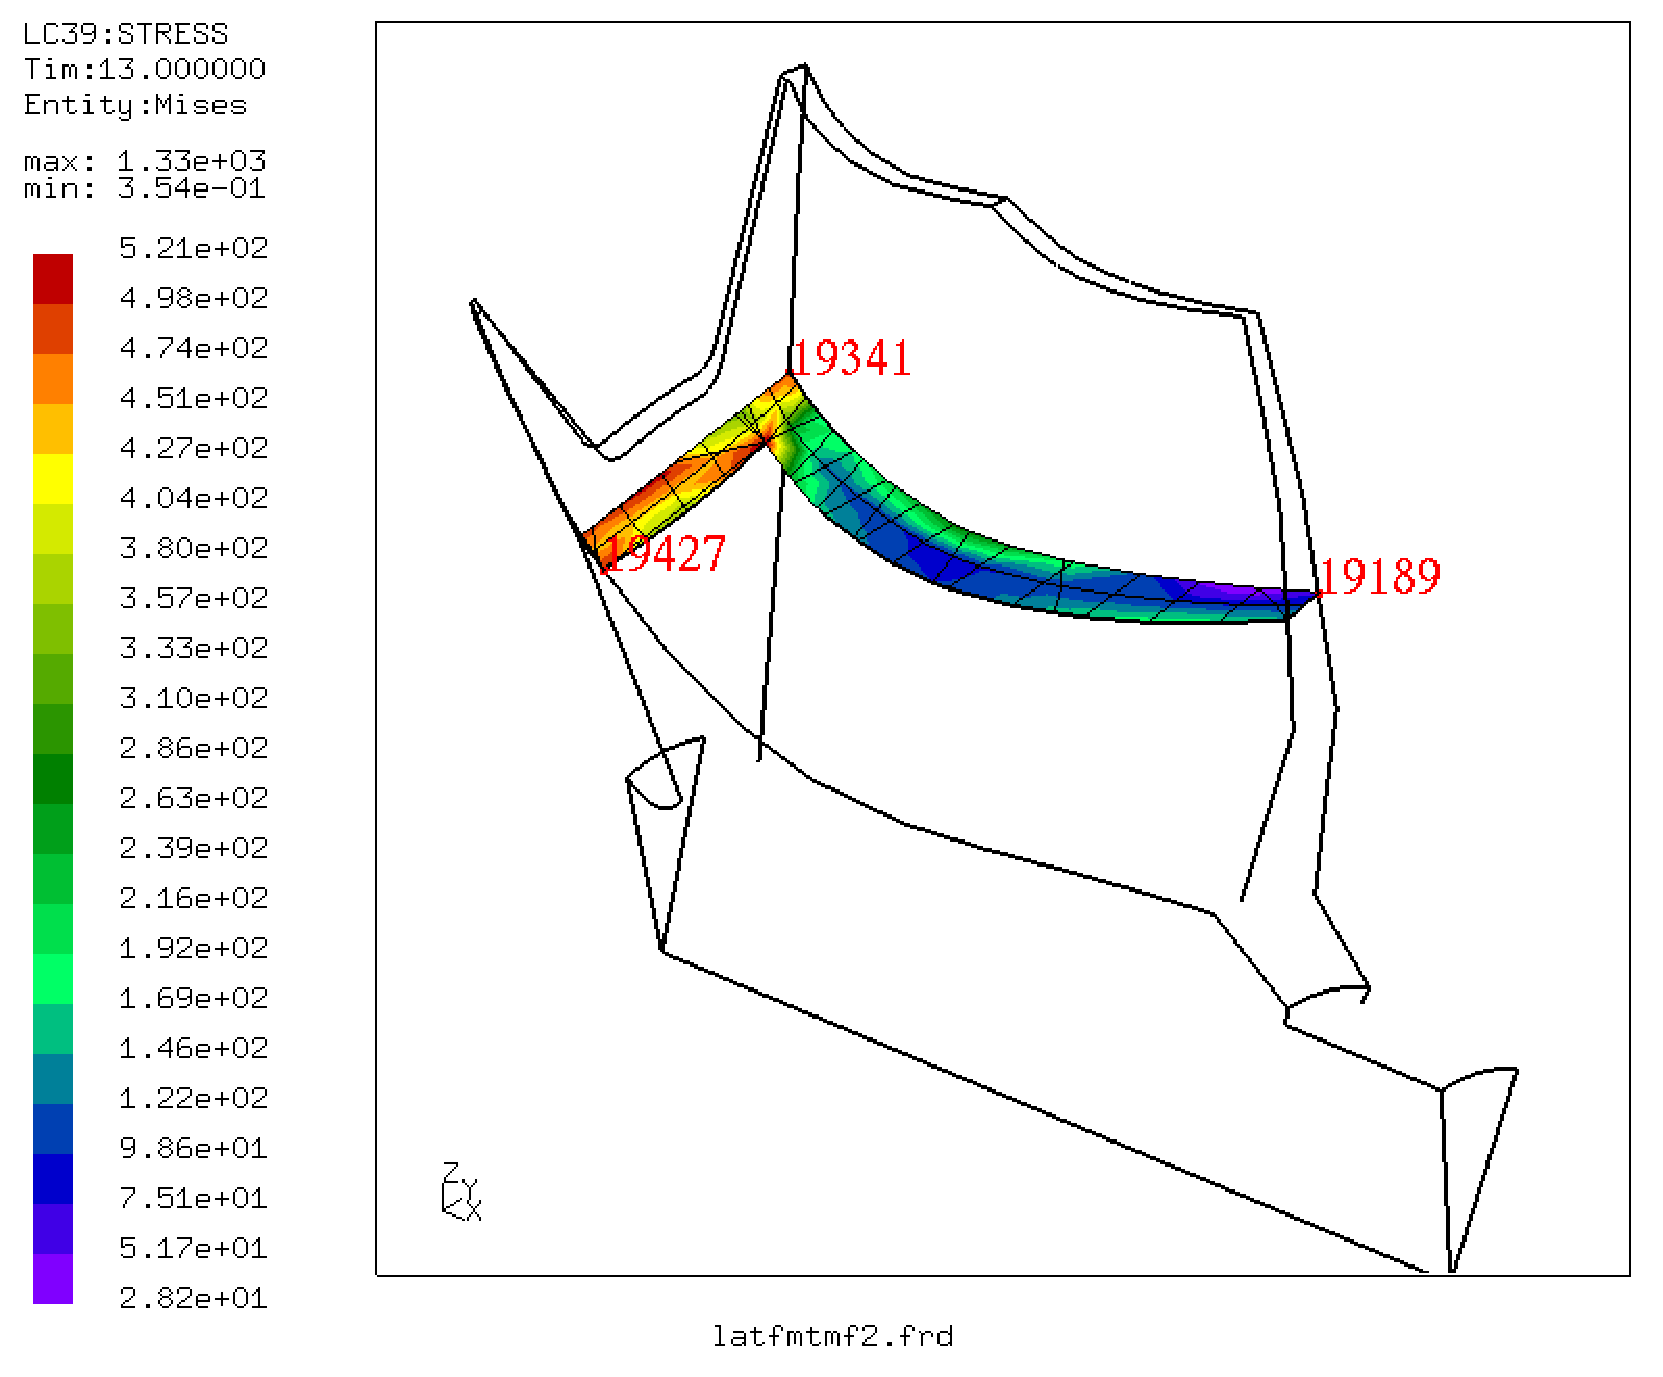
\epsfig{file=qcut.eps,width=12cm}
\caption{\label{qcutp}qcut: A section through a model defined by three nodes}
\end{figure}

\subsection{\label{qdel}qdel}
\begin{verbatim}
   'qdel' RETURN 'w'|'a'|'i'|'r'|'p'|'l'|'s'|'b'|'S'|'L'|'h'|'q' 
\end{verbatim}
This keyword is used to delete entities (see also \htmlref{del}{del}). Higher entities (depending ones) will be deleted to. To delete more than one entity with one stroke, type ''a'' before and create a rectangular picking area by pressing two times the ''r'' key. Both strokes define opposite corners of the rectangle. To delete only one entity type ''i'' before. Press ''q'' to quit the command. 

It is also possible to measure distances between two pixels on the screen. Just press the key ''w'' on the positions of the two pixels. The distance is calculated in the scale of the displayed geometry.

\subsection{\label{qdis}qdis}
\begin{verbatim}
   'qdis' RETURN 'w'|'c'|'n'|'p'|'q' 
\end{verbatim}
This keyword is used to measure distances between two nodes or points. Move the mouse pointer over one entity and press the following key, for a node n, for a point p or for a center point c. If the key c was pressed then the distance between the two nodes or points are given in cylindrical coordinates. Here lcir is the length of the arc da the angle dr is r2-r1. If no center point was chosen then the distance and its xyz components are given in the Cartesian system. But in addition the cylindrical distances around the origin and around the xyz-axis are also given. Press ''q'' to quit the command.

\begin{itemize}
\item dist: global distance
\item dx, dy,dz: distance in the three Cartesian directions
\item da: global angle
\item dax, day, daz: angle around x, y, z
\item dr: global radius difference
\item drx, dry, drz: radius difference around x, y, z
\end{itemize}

It is also possible to measure distances between two pixels on the screen. Just press the key ''w'' on the positions of the two pixels. The distance is calculated in the scale of the displayed geometry.

\subsection{\label{qdiv}qdiv}
\begin{verbatim}
   'qdiv' RETURN 'w'|'a'|'i'|'1'-'9'|' 10'-' 99'|'q' 
\end{verbatim}
This keyword is used to change the division of a line by pressing a number between 1 and 9 when the mouse pointer is at the position of a line (see also \htmlref{div}{div}). To define numbers between 10 and 99 press the space bar when the mouse pointer is at the position of a line and then the number. To select more than one line with one stroke, type ''a'' before and create a rectangular picking area by pressing two times the ''r'' key. Both strokes define opposite corners of the rectangle. To select only one line type ''i'' before. Press ''q'' to quit the command. General rules are described in ''\htmlref{div}{div}''. 

It is also possible to measure distances between two pixels on the screen. Just press the key ''w'' on the positions of the two pixels. The distance is calculated in the scale of the displayed geometry.

\subsection{\label{qenq}qenq}
\begin{verbatim}
   'qenq' RETURN 'w'|'a'|'i'|'r'|'n'|'e'|'f'|'p'|'l'|'s'|->
                 'b'|'S'|'L'|'h'|'m'|'u'|'v'|'t'|'q' 
\end{verbatim}
This keyword is used to gain information about entities. It is especially useful to get the values on particular nodes.

If the maximum or minimum value in a certain area has to be searched type first ``m'' to go in the max/min mode and create a rectangular picking area by pressing two times the ''r'' key. Both strokes define opposite corners of the selection-rectangle. Then the key ``h'' (high) to search the node with the maximum value. The minimum is searched with ``l'' (low). The search-result is then shown in the xterm and also attached to the node. With the ``u'' key the last search result can be deleted (``undo''). The 't'-key changes into the ``qtxt''-mode. The ''\htmlref{qtxt}{qtxt}'' functionallity is now available which allows to manipulate the node-attached-string and its position on the screen. Use ''\htmlref{qadd}{qadd}'' instead of ``qenq'' if you need to save the node in a set for further use.

To catch more than one entity with one stroke, type ''a'' (all) before and create a rectangular picking area by pressing two times the ''r'' key. Both strokes define opposite corners of the rectangle. To catch only the entity which is closest to the user type ''i'' before.

Then move the mouse pointer over the entity(s) and press one of the following keys, for Nodes n, Elements e, Faces f, Points p, Lines l, Surfaces s, Bodies b, Nurb Surfaces S and for Nurb Lines L.

The position of nodes or points are given in Cartesian and cylindrical coordinates (see figure \ref{qenqp}, axyz are the 3 angles around x,y and z, rxyz are the 3 radii around x, y and z). In a second row the sets to which the picked entity belongs are listed. 

Press ''q'' to quit the command. 

It is also possible to measure distances between two pixels on the screen. Just press the key ''w'' on the positions of the two pixels. The distance is calculated in the scale of the displayed geometry.
  
\begin{figure}[h]
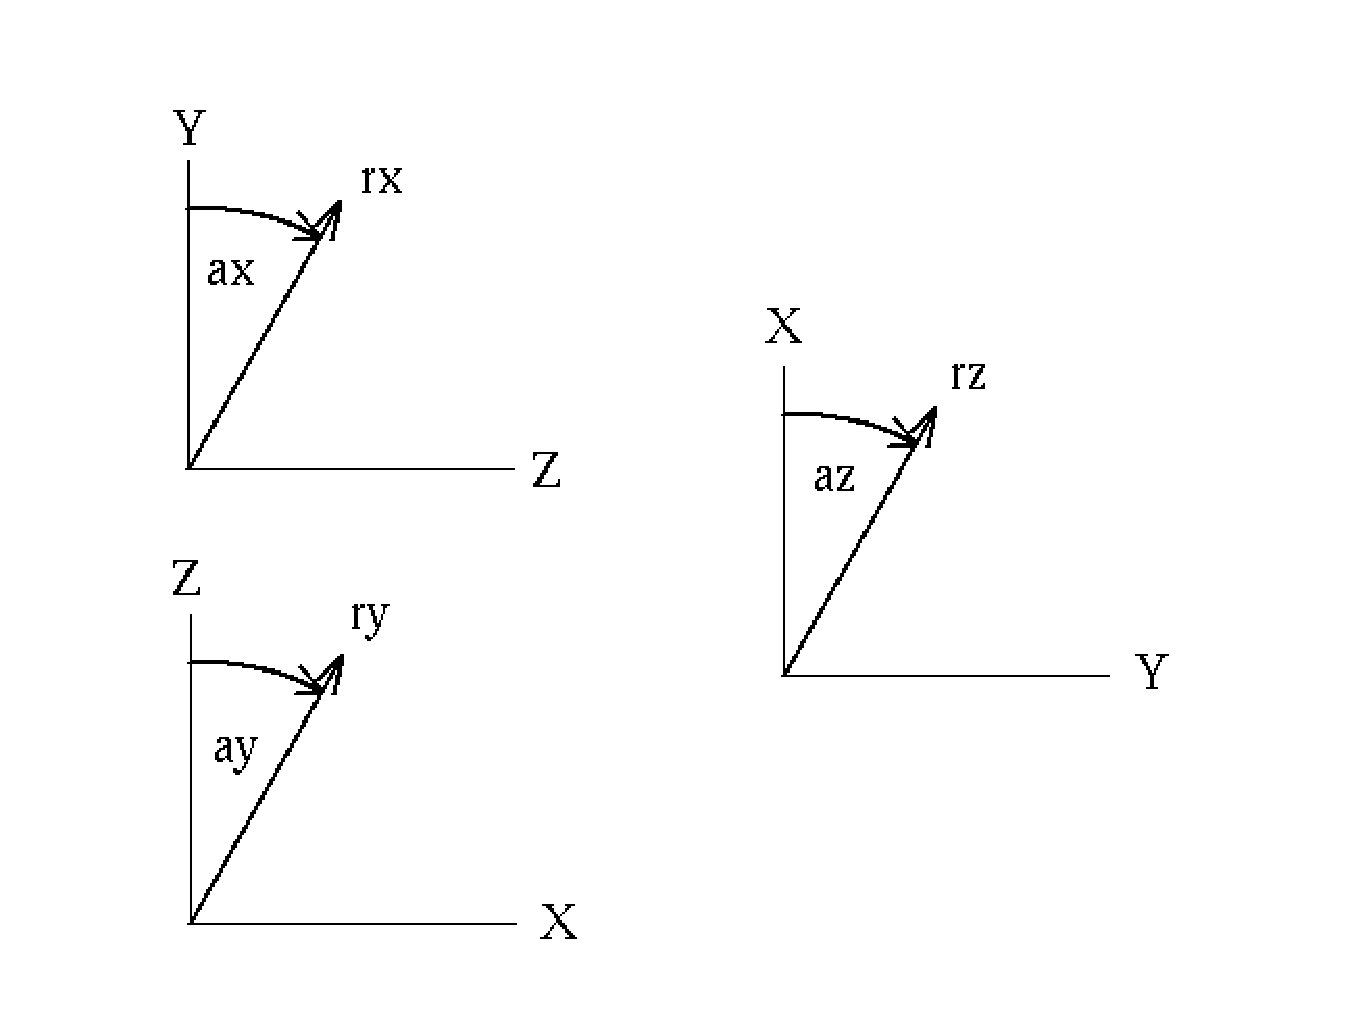
\epsfig{file=coords.eps,width=12cm}
\caption{\label{qenqp}qenq: Definition of the cylindrical system}
\end{figure}

\subsection{\label{qfil}qfil}
\begin{verbatim}
   'qfil' <radius> RETURN 'w'|'l'|'q'
\end{verbatim}
The command creates a fillet line (a radius) between two lines who intersect. After the command-name the value for the fillet-radius has to be specified. Then for each pair of selected lines a fillet of this value will be created. Select lines with the ''l''-key. Press ''q'' to quit the command. Currently it works only for straight lines. A curved line can be split and the part which should be used for the fillet can be transformed to a straight form with the ''\htmlref{qlin}{qlin}'' command (''s'' and ''x'' key-strokes). Figure \ref{qfilp} shows on the right side the initial situation and on the left side the created fillet. The command has also shifted point P002 to the left. Always the end-point of the first selected line closest to the intersection is moved. The second line gets a new end-point. 
  
\begin{figure}[h]
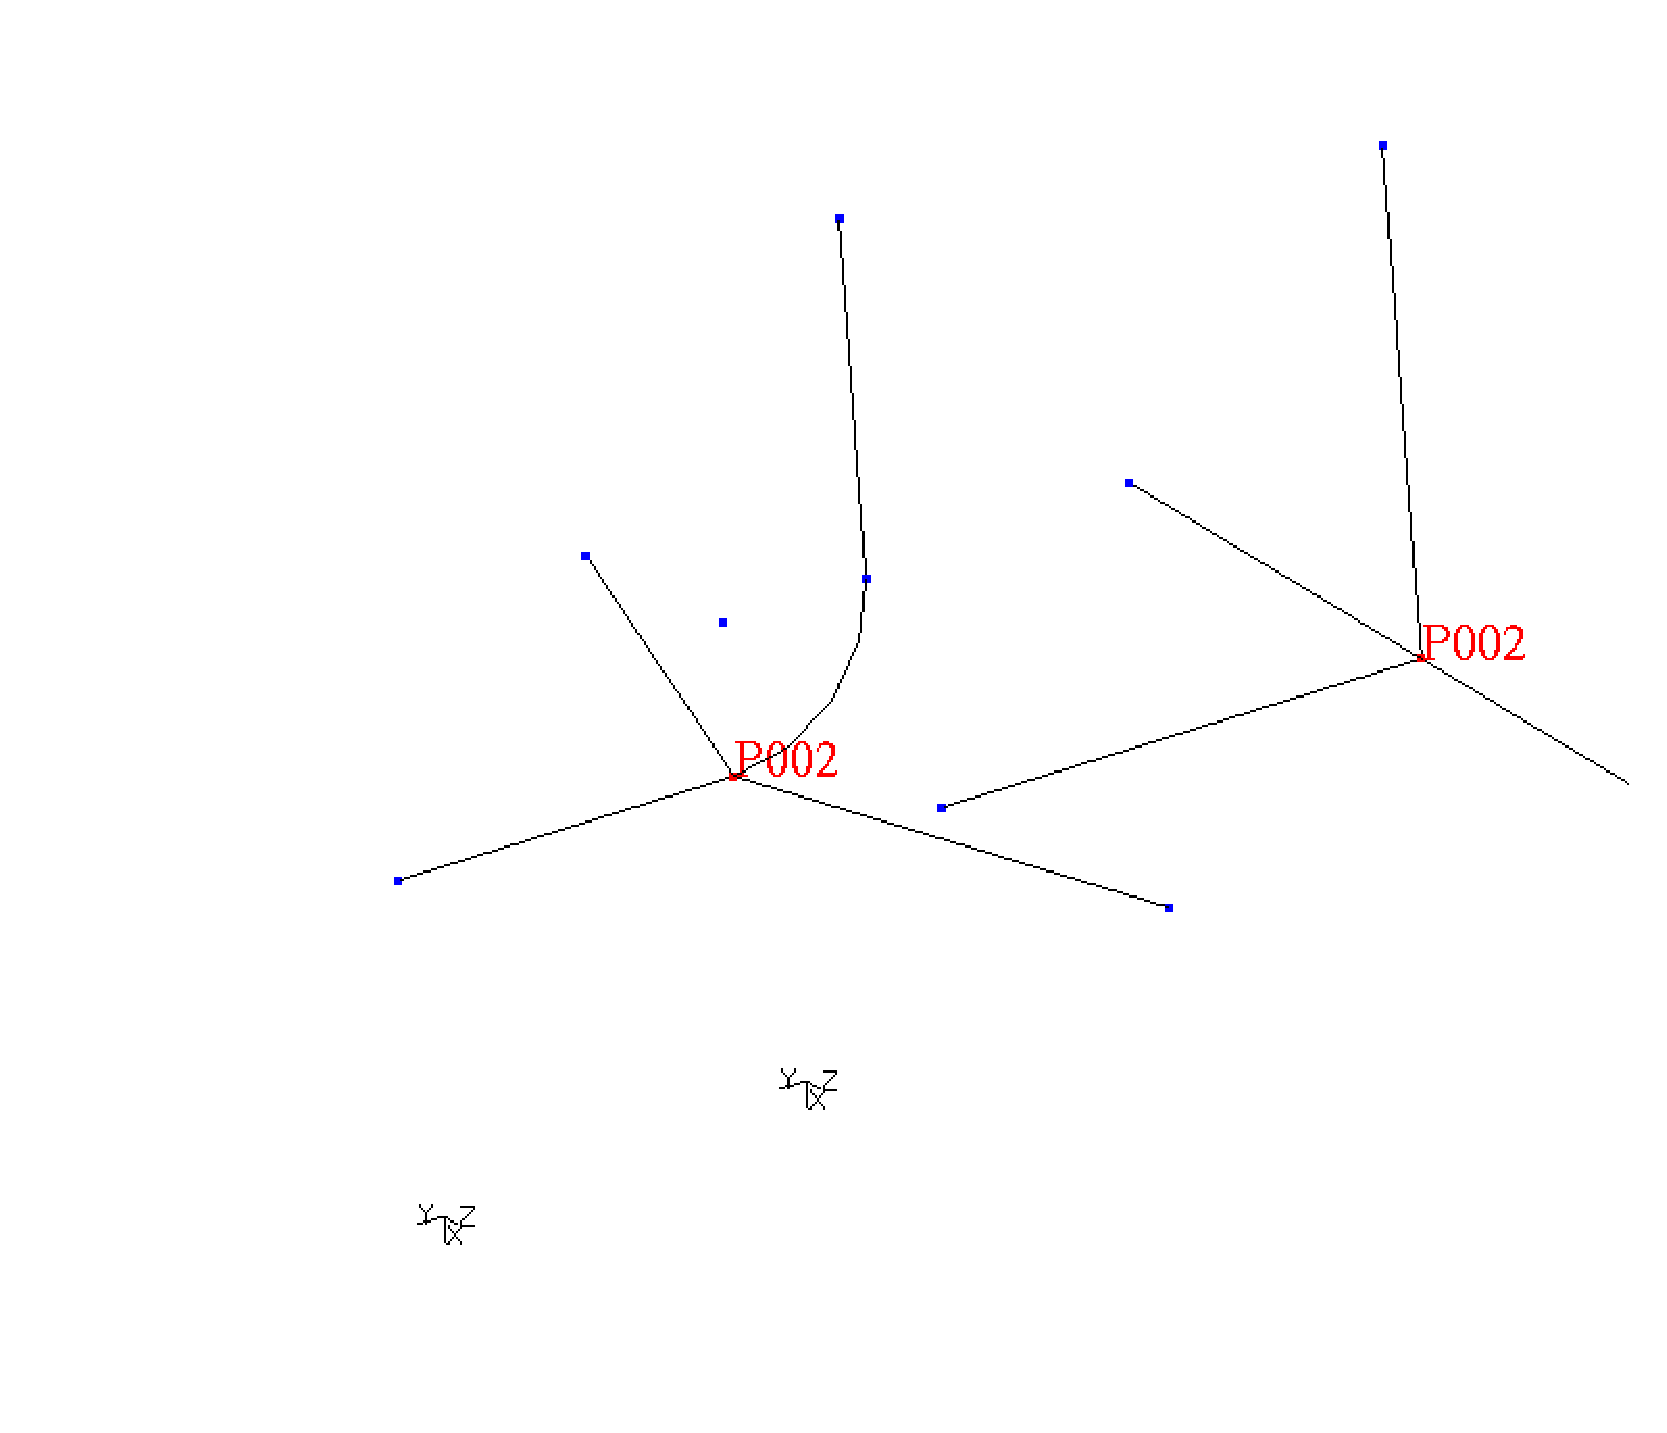
\epsfig{file=qfil.eps,width=12cm}
\caption{\label{qfilp}qfil: Based on two intersecting lines a fillet is created }
\end{figure}

\subsection{\label{qflp}qflp}
\begin{verbatim}
   'qflp' RETURN 'w'|'e'|'s'|'a'|'i'|'q'
\end{verbatim}
This keyword is used to invert the outer- and inner side (the orientation) of shell-elements and surfaces. The orientation of shell-elements or surfaces can be seen by the interior color. The outer face reflects light, if the face is dark-grey it is the back-side. If ''\htmlref{Toggle Culling Back/Front}{Toggle Culling Back/Front}'' was selected before then both sides are illuminated. To flip the orientation of a surface and all related shell-elements select either a shell-element with the ''e'' key or if the illuminated surfaces are displayed (see ``\htmlref{rep}{rep}'' how to do that) select the surface with the ''s'' key. To see the effect on the elements immediatelly they must have been displayed with the ''\htmlref{plot}{plot}'' command. If only elements are in the database flip them with the ''e'' key. The ''a'' key has a different meaning than usually. If pressed before a selection then a so called auto mode is activated. It makes sense for volumes were a vector pointing in or out can be determined for all surfaces. In this case all related surfaces (and embedded elements) are oriented in the same way as the selected one. It works only in situations were only two surfaces share a common edge. This is the case for volumes without inner surfaces or a 2D model. In case of a volume all surface normals will point either inwards or outwards, depending on the orientation of the selected surface. Press ''q'' to quit the command. 

It is also possible to measure distances between two pixels on the screen. Just press the key ''w'' on the positions of the two pixels. The distance is calculated in the scale of the displayed geometry.

\subsection{\label{qint}qint}
\begin{verbatim}
   'qint' RETURN 'w'|'l'|'q'
\end{verbatim}
This keyword is used to extend two lines to their intersecting location. The end-points of the two lines are moved to the intersecting location but they are not merged. Use the ''\htmlref{merg}{merg}'' command to merge duplicate points. Only straight lines are supported. Select lines with the ''l''-key. Press ''q'' to quit the command.

\subsection{\label{qlin}qlin}
\begin{verbatim}
   'qlin' <name>(optional) RETURN 'w'|'b'|'c'|'e'|'g'|'l'|'m'|'p'|->
                                  'q'|'s'|'t'|'u'|'x'
\end{verbatim}
This keyword is used to create a sequence of lines (or just one, see also \htmlref{line}{line}). The user might specify a name in the command-line or by picking an existing line with the key ''l''. In this case an existing line might be redefined without destroying related geometries.

To start a sequence of lines move the mouse pointer over a point and press the key ''b'' (begin).

To define just a straight line go to the end point and press ''g'' (generate). This point is also the starting point for the next line. So no ''b'' is necessary for the next line.

If the line is a sequential line (spline) then the points of the sequence must be defined with the key ''t'' in the correct order, but the last point must be selected with the key ''g''.

If the line is an arc then the center point must be selected with the ''c'' key or one point on the line between the end-points must be selected with the ''m'' key, but the last point must be selected with the key ''g''.

In case you need to split a line during the process, you can do that by pressing the ''s'' key.

When you want to modify the length then pick an existing line with the key ''l'' and then the endpoint you want to move with the key ''p''. The displacement is requested and the point is moved in the direction of the line by the specified displacement. 

The ''x'' key will transform the line into a straight line.

One quite usefull function for cad-based surfaces is triggered by the ''e''-key (exchange). This allows to modify an existing surface (\htmlref{gsur}{gsur}). With that command a line or a line sequence in a \htmlref{lcmb}{lcmb} can be exchanged by the previous selected (``l'' key) or generated line. For example one edge of an already existing surface uses a lcmb but the user wants to replace it by a spline (line) then the user defines or selects the new spline and then moves the mouse in an area were one of the old lines (the new one might be present as well) is located and presses the ''e'' key. The definition of the lcmb will be changed without destroying the surface-definition.

Press ''q'' to quit the command or ''u'' to delete the last created line.

It is also possible to measure distances between two pixels on the screen. Just press the key ''w'' on the positions of the two pixels. The distance is calculated in the scale of the displayed geometry.

\subsection{\label{qmsh}qmsh}
\begin{verbatim}
   'qmsh' RETURN 'f'|'v'|'n'|'l'|'c'|'s'|'m'|'d'|'q'
\end{verbatim}
A very usefull command to optimize surface meshes as a basis for tet-meshes. Based on identified lines ``l'' or surfaces ``s'' meshes can be deleted ``d'' and generated ``m''. Surfaces can be combined ``c'' to get rid of very small ones (usually first identified by a common line with ``l''). Example:
\begin{itemize}
\item Identify a line with key ``l''. The related surfaces are selected.
\item Then press key ``d'' if the mesh retated to this surfaces should be deleted.
\item The line divisions might be changed by pressing the key with the desired number. This function of qmsh works like the ``\htmlref{qdiv}{qdiv}'' command.
\item Press key ``m'' to re-mesh the surfaces
\item To combine two selected surfaces press key ``c'' (after selecting surfaces individually or by selecting a line).
\end{itemize}
A surface (without holes) can be splitted by a new line:
\begin{itemize}
\item First create the desired splitting line, for example with ``\htmlref{qlin}{qlin}''.
\item Convert the line to a spline with ``\htmlref{qseq}{qseq}'' (optional)
\item Project the line-points to the surface with ``\htmlref{qpnt}{qpnt}'' or ``\htmlref{proj}{proj}'' (optional)
\item Type ``qmsh'' and identify the line with key ``l''.
\item Identify the surface with key ``s''.
\item Press key ``b'' to break (split) the surface in two.
\end{itemize}

This keyword is also used to manually define elements. The key ``n'' selects nodes and the key ``s'' or ``v'' generate a surface or volume element based on the node-selection. Mostly used to repair stl files manually.

\subsection{\label{qnor}qnor}
\begin{verbatim}
   'qnor' RETURN 'w'|'p'
\end{verbatim}
A new line normal to a plane defined by three points and a length is created. It starts at the last point.

\subsection{\label{qpnt}qpnt}
\begin{verbatim}
   'qpnt' <name>(optional)RETURN 'w'|'p'|'g'|'m'|'n'|'s'|'S'|'u'
\end{verbatim}
This keyword is used to create or move points (see also \htmlref{pnt}{pnt}). The user might specify a name in the command-line if a certain name should be used. To create a point move the mouse pointer to the desired location and press the key ''g'' (generate) or over an existing node and press ''n'' (uses then the node-coordinates). After a point was selected with ''p'' it can be moved in different ways: Either in the screen-plane, for this go to the desired position and press ''m'' (move, see \htmlref{qali}{qali} or the section \htmlref{Orientation}{Orientation} how to rotate the model into a certain position). Or the point can be moved to the position of a second point, for this go to the second point which coordinates should be used and press ''p'' again. If the coordinates of a node should be used press ''n'' instead. Also a normal projection to a nurbs related surface (from cad-systems) is feasible by choosing the target-surface with the ''s'' key or a NURBS-surface with the ''S'' key either before or after the point was marked. Press ''q'' to quit the command or ''u'' to undo the last action.

If you picked the wrong point (the one which should be moved), just pick the same again and pick then the correct one.

It is also possible to measure distances between two pixels on the screen. Just press the key ''w'' on the positions of the two pixels. The distance is calculated in the scale of the displayed geometry.  

\subsection{\label{qnod}qnod}
\begin{verbatim}
   'qnod' RETURN 'w'|'p'|'m'|'u'
\end{verbatim}
This keyword is used to move nodes (see also \htmlref{node}{node}). To move a node move the mouse pointer to the desired node and press ''p'' (pick) then go to the desired position and press ''m'' (move). See \htmlref{qali}{qali} or the section \htmlref{Orientation}{Orientation} how to rotate the model into a certain position. Press ''q'' to quit the command or ''u'' to undo the last action. 

It is also possible to measure distances between two pixels on the screen. Just press the key ''w'' on the positions of the two pixels. The distance is calculated in the scale of the displayed geometry.  

\subsection{\label{qrem}qrem}
\begin{verbatim}
   'qrem' <set> RETURN 'w'|'a'|'i'|'r'|'n'|'e'|'f'|'p'|'l'|'s'|->
                       'b'|'q' 
\end{verbatim}
This keyword is used to erase entities from a set (see also \htmlref{setr}{setr}). To remove entities move the mouse pointer over the entity and press the following keys, for Nodes n, Elements e, Faces f, Points p, Lines l, Surfaces s, Bodies b, Nurb Surfaces S and for Nurb Lines L. To catch more than one entity with one stroke type ''a'' before and create a rectangular picking area by pressing two times the ''r'' key. Both strokes define opposite corners of the rectangle. To catch only one entity type ''i'' before. Press ''q'' to quit the command. 

It is also possible to measure distances between two pixels on the screen. Just press the key ''w'' on the positions of the two pixels. The distance is calculated in the scale of the displayed geometry.

\subsection{\label{qseq}qseq}
\begin{verbatim}
   'qseq' [<set> RETURN 'n'|'p']|[ RETURN 'nr'] 
\end{verbatim}
This keyword is used to define a sequence. The sequence might consist of nodes or points. A sequence is nothing else than a set which keeps the selection-order of the entities:\\\\qseq nodeset\\\\will store all selected nodes (selected with the 'n' key) in the order in which they were selected. This set might be used for a subsequent ''\htmlref{graph}{graph}'' command. Point sequences are used to define splines. If\\\\qseq\\\\is typed without a setname then an existing line has to be selected with a nummerical keystroke (or the space-bar followed by two numbers). New points will be created on this line which in turn are used to redefine the selected line as a sequence-line which uses the new spline-points. Sequences can be shown with the ``\htmlref{prnt}{prnt} sq'' command. Node sequences can be written to a file and read again with the commands ``send seqname fbd'' and ``read seqname.fbd''.

\subsection{\label{qshp}qshp}
\begin{verbatim}
   'qshp' RETURN 'w'|'n'|'p'|'g'|'h'|'s'|'S'|'c'|'q'
\end{verbatim}
This keyword is used to define a shape. A shape needs 3 points (or nodes, points at their location will be generated and used) for its definition. The points are selected with the 'p' (nodes 'n') key. After the points are selected it will be generated by a 'g' keystroke. The shape can be assigned to a surface by selecting first either a shape 'h' or a nurbs 'S' and then the surface with the 's' key. The shape will then define the interiour of this surface. The selected shape or nurbs stay selected until cleared with 'c'.

It can also be used for projection purposes (see ''\htmlref{proj}{proj}'') or splitting (see ''\htmlref{split}{split}'').

\subsection{\label{qspl}qspl}
\begin{verbatim}
   'qspl' RETURN 'w'|'s'|'q' 
\end{verbatim}
This keyword is used to split one or more lines at a certain position (can also be done with ''\htmlref{qlin}{qlin}''). A point is created at the splitting position, the original line is deleted and two new lines will appear instead. All lines running through the selected location will be split at once and the newly created splitting points will be merged to one if they are closer to each other than defined by ''\htmlref{gtol}{gtol}''. To split a line move the mouse pointer over the line and press the ''s'' key. Press ''q'' to quit the command. 

It is also possible to measure distances between two pixels on the screen. Just press the key ''w'' on the positions of the two pixels. The distance is calculated in the scale of the displayed geometry.

\subsection{\label{qsur}qsur}
\begin{verbatim}
   'qsur' <name>(optional) RETURN
   'w'|'a'|'b'|'l'|'i'|'r'|'1'-'9'|'g'|'q'|'u'|'s'|'S'|'h'|'c'
\end{verbatim}
This keyword is used to create or change a surface (see also \htmlref{gsur}{gsur}). The user might specify a name in the command-line or by picking an existing surface with the ''s'' key.

If the surface is supposed to be meshed with unstructured triangles (element type tr3u or tr6u) it is sufficient to select all lines with the ``l'' key (lowercase ``L''). This can be done either in the ``all''-mode (press ``a'') or ``individual''-mode (press ``i'') which is default. Then generate the surface by pressing the ''g'' key. Such surfaces allow holes in it. If the surface is not plane it will need to reference an embedded NURBS surface (see ''\htmlref{nurs}{nurs}'') or a shape (see ''\htmlref{shpe}{shpe}''). Despite it is quite an exception it should be noted here that this kind of mesh might be extruded in the 3rd dimension by using the ''\htmlref{swep}{swep}'' command to generate penta elements for the cfd solver. Only external meshers might use the triangles as a geometry description (see ''\htmlref{How to deal with cad-geometry}{How to deal with cad-geometry}'').

For the definition of a regular meshable surface three to five edges must be
defined. To create a surface move the mouse pointer over the first line of the
first edge and select it with the ''1'' key (number ``one''). If more than one
line is necessary to define the first edge select the following ones one after
the other with the ''1'' key. Each marked line is listed in the mother
xterm. If all lines of the first edge are selected select the lines of the
second edge by pressing the ''2'' key, then the third and eventually the
fourth and fifth. The last selected line must match the first. All lines
defining an edge will create a combined line (see \htmlref{lcmb}{lcmb}) and
this combined line will show up in the definition of the surface. Then
generate the surface by pressing the ''g'' key and you might continue with the
next surface. By default the interior of the surface is defined according to
Coons \cite{Coons} which is a blended function. But it can also follow an
embedded NURBS-surface or a shape. To relate a surface to an existing NURBS
surface select another surface which already uses the desired NURBS with the
''S'' key (uppercase) or to reference the shape with the ``h'' key. Then
select the target-surface with ``s''. The target surface is converted to a
NURBS surface which is necessary to be meshable with unstructured triangles
(tr3u, tr6u) and to be used to generate tet elements. The selected shape or nurbs will stay selected until cleared with 'c'.

An existing surface might be completly redefined without destroying the definition of related bodies or other geometries. After selecting a surface with the ``s'' key the referenced lines might be replaced by selecting new ones. The previous selected lines are not longer referenced.

Replace assignments by the blended function with the ''b'' key. To quit the command use the ''q'' key or use ''u'' to undo the last action. 

It is also possible to measure distances between two pixels on the screen. Just press the key ''w'' on the positions of the two pixels. The distance is calculated in the scale of the displayed geometry. 

\subsection{\label{qtxt}qtxt}
\begin{verbatim}
   'qtxt'  RETURN 'g'|'a'|'i'|'b'|'p'|'m'|'n'|'v'|'f'|'d'|'q' 
\end{verbatim}
This keyword is used to move node-attached texts (showing node-number and value, see figure \ref{qtxtp}) to certain positions in the drawing area or to manipulate them otherwhise. They are created with the key ``g'' while the mouse-pointer is over the node to which it should be attached. Attention: They are only visible after the command ''\htmlref{plus}{plus} nt all'' was used (but they are immediatelly visible when the the commands ''\htmlref{qenq}{qenq}'' or ''\htmlref{qadd}{qadd}'' were used instead of ``qtxt''). To move a text pick it at the lower-left corner with the key 'p' and place it with the key 'm' in the new location. To move it back to its node use 'b'. Delete them with 'd'. The node-nr and the value in the text can be switched on and off with the 'n' and 'v' key. The 'f' key will toggle the format of the value between ``int'', ``float'' and ``exponent''. See the command ''\htmlref{font}{font}'' on how to change the font-size.

To catch more than one entity with one stroke, type 'a' (all) before and create a rectangular picking area by pressing two times the 'r' key. Both strokes define opposite corners of the rectangle. To catch only the entity which is closest to the user type 'i' before.
  
\begin{figure}[h]
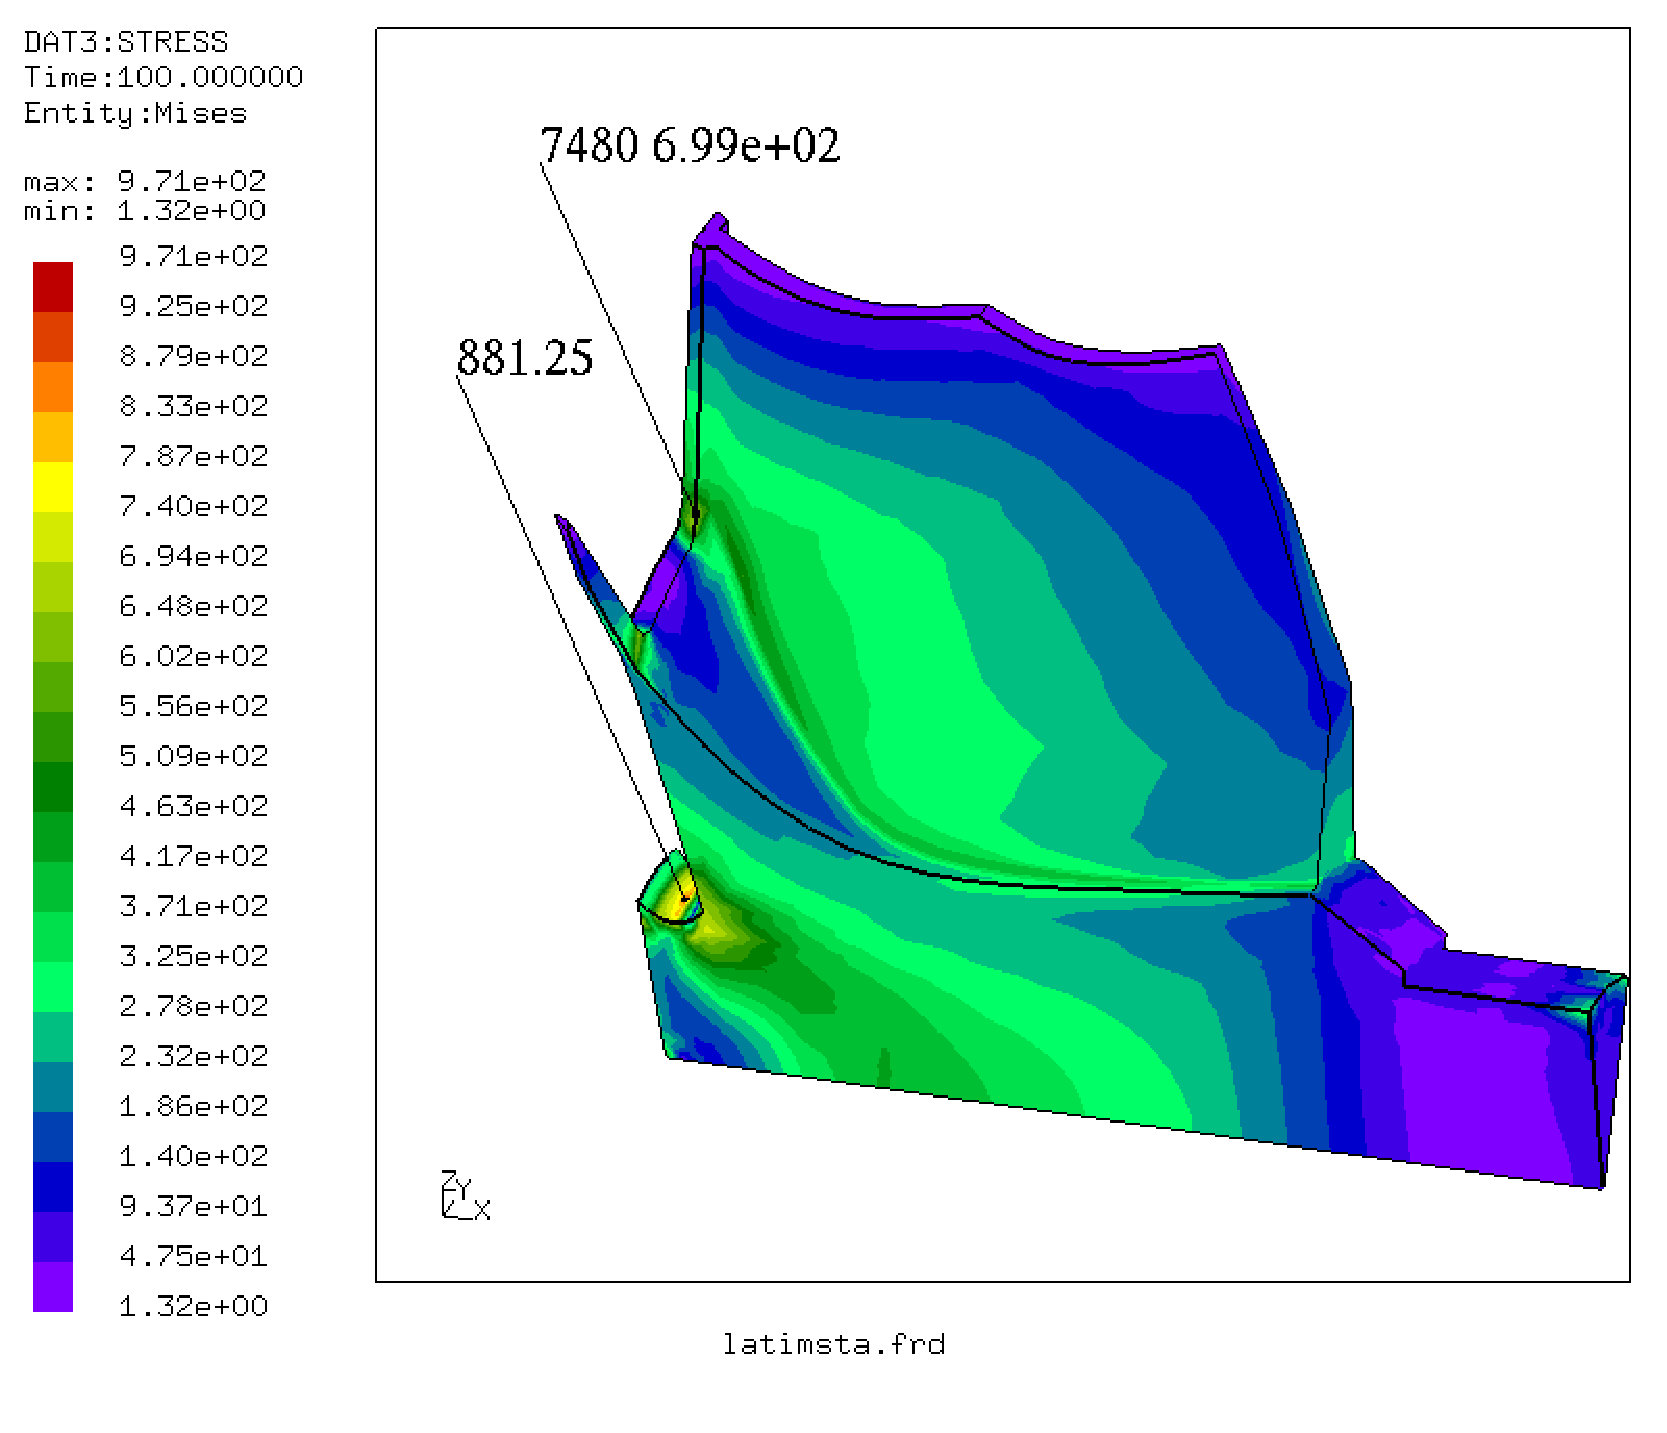
\epsfig{file=qtxt.eps,width=12cm}
\caption{\label{qtxtp}qtxt: Node attached texts at two locations, one with node-nr and value in exp-form and one just with his value in floating point form. The font with gives biggest numbers was used.}
\end{figure}

\subsection{\label{quit}quit}
\begin{verbatim}
   'quit' 
\end{verbatim}
This keyword is used to terminate the program without save. 

\subsection{\label{read}read}
\begin{verbatim}
   'read' [<geo-file> ['add']]|
          [<ccx-file> 'inp' ['add'|'ext'|'nom'|'new']]|
          [<openFoam-file> 'foam' ['add'|'ext'|'nom']]|
       [<result-file(frd)> ['add'|'ext'|'nom']|[<setname>]]|
          [<stl-file> ['add'|'ext'|'nom']]|
          [<list-file> '-n'|'-e'<column>]|
          [<edge-file> 'edg']|
          [<netgen-file> 'ng' ['add'|'ext'|'nom'|'ndsb']]|
          [<pixel-file> [<zoom>]|[<x_zoom> <y_zoom>]]
\end{verbatim}
This keyword is used to read files or commands from a file. Most commands can be read from a file but not all of them. In general all basic commands to create geometry are understood and up to now this is the only way to read pre defined geometry during run-time. To read commands from a file like \htmlref{pnt}{pnt}, \htmlref{line}{line}, \htmlref{node}{node}, or \htmlref{seta}{seta} and so on, type\\\\read geo-file\\\\this will eventually replace entities if their names were already in use. To prevent this, type\\\\read geo-file add\\\\this forces the program to change the names which are already in use to unused ones. Therefore no existing geometry will be overwritten.

If an ccx-input-file with loads, boundary-conditions and sets was read\\\\read ccx-file inp\\\\then the loads and boundary-conditions are stored in automatically created sets which start with a leading '+'. For example the ccx command '*BOUNDARY' will trigger the creation of the set '+bou'. The ccx sets are stored in cgx sets of the same name. The load-values are stored in Datasets.

The option ``nom'' (no-mesh)\\\\read ccx-file inp nom\\\\is used to suppress the reading of nodes and elements. This speeds up the reading and makes sense if the mesh exists and only the set-definitions and loads should be read. 

If the parameter ''add'' is used,\\\\read ccx-file inp add\\\\ then existing node- or element-numbers are not overwritten and the program choses new numbers. If the ccx-input-file ends with ``.inp'' the parameter ``inp'' might be omitted.

An openFoam file \cite{OpenFOAM} can be read in a similar way\\\\read CaseDirName foam\\\\as an ccx input file. Sets will be created if defined in the openFoam file. Results can be used for mapping purposes. For further details see ``\htmlref{How to map loads}{How to map loads}'' in the appendix.

The user might read a result-file in frd format during runtime. If a mesh exists and should not be overwritten just add the parameter ``add''\\\\read result-file add\\\\this forces the program to change the numbers which are already in use to unused ones. Existing datasets will be extended by the new node-numbers and their data. The option ``ext'' \\\\read result-file ext\\\\will also extend the existing datasets but in this case the nodes and elements are updated (modified). If no parameter follows then existing nodes and elements are updated and the new datasets will be appended to existing ones. Since the dependency checks are time consuming the user might scip them by using the 'ne' parameter. Then the existing mesh is deleted before the new one is read:\\\\read result-file new\\\\

It is also possible to read files written in the result format (.frd) during runtime only to define sets of nodes or elements without changing the definitions of them. The command\\\\read result-file setname\\\\will create a set of the name setname and all nodes and elements listed in the file mesh.frd will be added to that set. But this will NOT create or modify the nodes and elements. All nodes and elements must exist and will not be changed.

An stl file can be read with \\\\read file.stl\\\\.

If a file with the numbers of nodes or elements is not available in the result format (.frd) then a so called list-file could be read instead. In such a file either numbers of nodes or elements can be defined. The numbers found in a specified column is interpreted as a node- or element-number. If ''-n'' is specified the numbers are interpreted as nodes and if ''-e'' is specified the numbers are interpreted as elements. For example\\\\read list-file -e3\\\\will define a set storing names of elements from the third column of file list-file.txt. The created set-name is always the name of the file.\\\\

\textbf{NETGEN Import}\\\\
In case NETGEN is used for meshing then the edges which are generated by NETGEN can be included for modifications;\\\\read edge-file edg\\\\will create beam elements based on the defined edges. When the modifications are done, the beam elements can be exported in the NETGEN-edge format with the ''send setname stl'' command and used for meshing in netgen (see also ''\htmlref{How to deal with cad-geometry}{How to deal with cad-geometry}''). The netgen mesh can be imported with
\begin{verbatim}
read netgen-file ng
\end{verbatim}
If the NETGEN (.vol) file contains solid elements, all shells and beams are only used to define surface sets of nodes and faces (+set\verb_<_nr\verb_>_). The shell elements and beams are deleted by default. If you want to be more selective about the elements imported from netgen, you use the keyword ndsb (NoDeleteShellsAndBeams).
\begin{verbatim}
read myfile.vol ng ndsb
\end{verbatim}
This keyword forces all the netgen elements to be imported. Be aware that the imported NETGEN element types (1D, 2D and 3D elements) are distributed in various sets for further operations (as well as being contained in set 'all'). For instance the set '+typ11' will contain all elements of type 11 (2-node beams). Please see ''\htmlref{Element Types}{Element Types}'' for a key to the element numbers.\\\\

If a pixel-file in xwd-format is available it can be included as a background-picture. The user can then create geometry based on this picture:\\\\read pixelfile 2 4\\\\here the picture will be scaled by a factor of ``2'' in x- and ``4'' in y-direction. Delete it with ''\htmlref{del}{del} pic''. The picture can not be modified in cgx. Only scaling during reading (with either a global factor or separate scaling in x- and y-direction) is supported. Other modifications have to be made with external software.


\subsection{\label{rep}rep}
\begin{verbatim}
   'rep' <set>  
\end{verbatim}
This keyword is used to refresh entities of a certain set. This is done automatically but with one exception: The rendering of the interior definition of surfaces must be triggered manually with this command. The rendered surfaces can be displayed with ''\htmlref{plot}{plot}'' or  ''\htmlref{plus}{plus}'' using the type ''si''.

\subsection{\label{rnam}rnam}
\begin{verbatim}
   'rnam' <set> <set>  
\end{verbatim}
This keyword is used to rename a set.

\subsection{\label{rot}rot}
\begin{verbatim}
   'rot'  ['u'|'d'|'r'|'l'|'c' <angle>]|
          ['x'|'-x'|'y'|'-y'|'z'|'-z'] 
\end{verbatim}
This keyword is used to rotate the view-direction to the model. For example\\\\rot u 10\\\\will rotate the view-direction 10 degrees upwards. The meaning of the other letters is down d, right r, left l, clockwise c. The remaining letters will rotate the view into a pre-defined direction. For example the user will look in x direction after the command\\\\rot x\\\\and against the x direction with the command\\\\rot -x\\\\and so on.

\subsection{\label{save}save}
\begin{verbatim}
   'save' 
\end{verbatim}
This keyword is used to save the geometry (if any) to a file named as the input file but with the extension .fbd. If a file with that name exists already, then this file will be saved with the new file extension .fbb as a backup.
 
\subsection{\label{scal}scal}
\begin{verbatim}
   'scal' ['s'|'v'|'d'] [<value>]
\end{verbatim}
This keyword is used to scale the graphic presentation of values but no values of entities. The scaling of the value itself can be done with the command ''\htmlref{ds}{ds}''. For example the command\\\\scal s 0.5\\\\will scale the range of values presented in the color plot by a factor of 0.5. The command\\\\scal v 5.\\\\will scale the length of vectors by a factor of 5. The command\\\\scal d 2.\\\\will scale the deformed shape by a factor of 2. Without a value it restores the default value. See also ''\htmlref{Toggle Vector-Plot}{Toggle Vector-Plot}'', ''\htmlref{Toggle Add-Displacement}{Toggle Add-Displacement}'', ''\htmlref{Datasets}{Datasets}''.

\subsection{\label{send}send}
\begin{verbatim}
  'send' <set> 'fbd' ['c','e']| ->
               'stl'| ->
               'abq'|'ans'|'ast'|'dar'|'duns'|'frd'|'gmp'|->
               'lst'|'nas'|'ng'|'pat'|'tcg' <RETURN>|
               ['bin']|
               ['ds'<nr>[+] [e<nr>[','|'-'<nr>]..]]|
               ['tmf']|
               ['sta' <refspeed>]|
               ['crp' <timefact> <refspeed> <writefreq>]|
               ['comp']|
               ['mpc' [[<rotation>|'v'<node> <v1> <v2> <v3> ]|
                                  ['n'<node>]]]|
               ['names']|
               ['spc' <dofs(1-6|t|p)> <value>]| ->
                 [<dofs(1-6|t|p)> 'ds'<nr> e<nr>]| ->
                 ['nor' <fac1> [<fac2> <fac3>]
               ['spcf' <dofs(1-6|t|p)> <value>]| ->
                 [<dofs(1-6|t|p)> 'ds'<nr> e<nr>]
               ['slide' 'c'|'s'|'rx'| ->
                 'ry'|'rz'|'tx'|'ty'|'tz']|
               ['pres' [<value>]|['ds'<nr> 'e'<nr>] [+|-] ]|
               ['film' [[n<nodnr>][<temp>]|->
                     [[['ds'<nr>]|[sq<dsnr>-<dsnr>]] 'e'<nr>]->
                 [[<coeff>]|->
                 [['ds'<nr>]|[sq<dsnr>-<dsnr>] 'e'<nr>]] [+|-] ]| 
               ['rad' [[<temp>]|['ds'<nr> 'e'<nr>]] ->
                 [[<emis>|['ds'<nr> 'e'<nr>]] [+|-] ]|
               ['dflux' [[<load>]|['ds'<nr> 'e'<nr>]] [+|-] ]|
               ['mflow' [[<load>]|['ds'<nr> 'e'<nr>]] [+|-] ]|
               ['cflux' <load>]| 
               ['force' <f1> <f2> <f3>]|
               ['quadlin']|
               ['sur' [+|-] ]
  'send' <set> ['dolfyn'|'duns'|'isaac'|'foam'] [<type> <set>] | ->
               ['cyclic' <set> <set> 'tx'|'ty'|'tz'|'rx'|'ry'|'rz'|
               'cx'|'cy'|'cz'|<vx,vy,vz>] 
  'send' <dep-set> <indep-set> 'nas'|'abq'|'ans' ['cycmpc'|'cycmpcf' ->
    'px'|'py'|'pz'|'tx'|'ty'|'tz'| ->
    'rx'|'ry'|'rz'|'cx'|'cy'|'cz'<+-segments> 'c'|'u'<NR>]| ->
    ['areampc' <dofs('t'|'p'|'1-6')> 'c'|'u'<Nr>]|'f'<value> ->
    ['areampc' 'slide']| ->
    ['areampc' 'presfit' ['s'<value>]]| ->
    ['gap' <vx> <vy> <vz> <tol>] 
\end{verbatim}
This keyword is used to send data to the file-system. The following formats are known (but not all options for all formats are fully supported so far); The geometry-format (fbd)\\\\send set fbd\\\\or\\\\send set fbd c\\\\will complete the set downwards before writing, or\\\\send set fbd e\\\\will write all model-edges as small lines running from node to node, and a surface description with triangles (stl)\\\\send all stl\\\\This triangles are based on elements which were created by meshing surfaces or by automatically triangulated element-faces of all types of supported elements. If be2 elements are included in the mesh (meshed lines) a so called edge file for NETGEN will also be created if stl is written. NETGEN provides also a stand-alone mesher called ng\_vol. The mesher can be found in the netgen sub-directory nglib. As for the stl-format triangles can be written for this mesher with:\\\\send set ng\\\\It has the advantage that the triangles are directly used to define tetras and not as with stl are only used to define the outer shape of the body.

The following mesh-related formats are known: Femview and CADfix (frd), Nastran (nas), Abaqus (abq), Ansys (ans), CodeAster (ast), Samcef (sam), Darwin (dar), patran (pat, only sets), gagemap (gmp, only sets) and Tochnog (tcg) but only ccx (Abaqus) is fully supported. Good support is also provided for ansys, darwin and nastran. If no further parameter follows then just the definition of the nodes and elements will be written:\\\\send all abq\\\\will write the mesh in the format used by Abaqus and the CalculiX solver. If the parameter ''ds'' is provided followed by the dataset-nr\\\\send set abq ds1\\\\then the values stored in Dataset 1 are written. For 'frd'-format the 'ds' parameter w/o any further values forces cgx to write all datasets but w/o the internally calculated ones:\\\\send all frd ds\\\\If a ``+'' sign appears at the end of the 'ds' parameter\\\\send all frd ds+\\\\or \\\\send all frd ds1+\\\\then also the internally calculated values like vMises-stress are written. Additionally the entities might be specified with the 'e' parameter followed by the numbers to write. The numbers have to be separated by a ',' sign or in case of a range by a '-' sign:\\\\send all frd ds1 e9,25-30\\\\ The ``bin'' parameter has the same meaning as the ``ds'' parameter but in this case the result is written in the binary form of the frd-format (always all datasets). In case data should be written for the crack analysis tool Darwin\\\\send all dar ds\\\\will write all datasets. Since Darwin changed the format from version 7.1 on, it is possible to change the format with the parameter 'v7.1' as the last parameter. If the set is of the ordered type and includes nodes (see ``\htmlref{qseq}{qseq}'') then the data are written in tabular form for use in a 1D crack-prop Darwin-analysis.

In certain circumstances the user needs an easy solver independent format to write node- and element numbers. This is provided by the ``lst'' parameter:\\\\send setname lst\\\\will write the node- and element-numbers in lines of seven space separated rows.

Missing lower entities (nodes, points, lines etc.)  will be added to the set before the set is written if the parameter ''comp'' follows. For example geometry like bodies\\\\send set fbd comp\\\\will be extended by surfaces, lines and points or\\\\send set frd comp\\\\will include all nodes used by the elements to the set elem and will then write the file.\\\\
The parameter ``quadlin'' forces the conversion from second order elements into single order elements were each element is subdivided into 8 single order elements. This takes place during writing and will not change the current state of the mesh in cgx. Up to now it is only available for the abq format:\\\\send all abq quadlin\\\\
If the parameter ''tmf'' follows the definition of a solver format\\\\send set abq tmf\\\\then the mesh plus all temperatures with the necessary solver context for tmf calculations is written. If the parameter ''sta'' follows \\\\send set abq sta 2900.\\\\then the mesh plus all temperatures with the necessary solver context for a static calculations is written. Here the value for ''speed'' is a reference value for eventual numerical values in the TEXT-Block of the Datasets in the result file (frd-file, see ''\htmlref{Nodal Results Block}{Nodal Results Block}''). A scaling factor will be determined based on the reference value (here a ref.speed of 2900.) and the individual TEXT-Block values (factor = speed**2 / refspeed**2). This factor is used in *AMPLITUDE commands which will also be written and will be used to scale static loads which are referenced in the *STEP data. If the parameter ''crp'' follows \\\\send set abq crp 1. 2900. 1\\\\then the mesh plus all temperatures with the necessary solver context for creep calculations is written. Here the value for ''timefact'' scales the time-values of the Datasets, ''speed'' is a reference value for scaling static loads (see option ``sta'') and writefreq limits the output to the result-file.\\\\
If the parameter ''names'' follows the solver-type then just the element- or node-numbers are written. This is useful for defining sets for the solvers. The command\\\\send steel abq names\\\\will write the node and element numbers included in ''steel''. This file could be used to define a set for material assignments, boundary conditions or loads. If all sets should be written at once, use:\\\\send all abq nam\\\\
If the solver-format ''duns'' is used then related numbers of surfaces (3D) or lines (2D) will be written. This information is necessary to apply boundary-conditions to duns. The numbers are used in the connectivity file (duns.conn) which will be created by the mesh-command. The user has to refer this numbers in the duns.script2 file when assigning boundary conditions.

It is also possible to define and send some constraints to the file system. To constrain degrees of freedom (dof) of selected nodes use the parameter ''spc'' in combination with the numbers of the constrained dofs and optionally a forced deflection. For example:\\\\send hinge abq spc 123\\\\will constrain the translational degrees of freedom of the nodes in set ''hinge''. Or\\\\send hinge abq spc 12356\\\\will leave just one rotational degree of freedom unconstrained. And\\\\send move-nodes abq spc 1 0.1\\\\will move the nodes in set move-nodes by 0.1 in direction 1.\\\\send move-nodes abq spc 1 ds1 e1\\\\will use the values from dataset-nr 1 and the entity-nr 1 for the forced displacement in direction 1 and\\\\send move-nodes abq spc nor 0.1\\\\ will force the nodes included in set move-nodes by 0.1 in the normal direction (normal to the element-faces). The components of the vectors at the node positions can be scaled individually (fac1-3)). A subsequent calculation with ccx will move the mesh accordingly. After solving the deformed mesh can be used as a new mesh for further calculations. With this procedure geometric variations are possible without manipulating the geometry (morphing).

For cfd there is a ``spc'' function available which works on faces instead on nodes.\\\\send Inlet abq spcf 123\\\\The degees of freedom 123 define velocities and not deflections. Its called ``spcf'' and works otherwhise accordingly to the ``spc'' command.

The parameter ''slide'' in combination with one additional parameter will create equations that force the selected nodes to move only in a plane. If the additional parameter ''s'' is specified then the specified nodes will be attached to their element faces. All nodes of the affected element-faces have to be selected. For example you type:\\\\send sur abq slide s\\\\and this should attach the node with the node-nr. 1 to a plane parallel to the surface of the corresponding element-face. This element uses the node 1, 2, 3, 4, 5, 6, 7 and 8 where 1, 2, 3 and 4 are on the surface of the mesh. The program will detect this element face and constrain the node only then if the nodes 2, 3 and 4 were also included in the set ''sur''! The detected elements or faces of volume-elements will be assigned to the set. So it is possible to check the detected elements. Instead of providing a set with the necessary nodes, you might instead provide a set with shell-elements or/and faces of volume-elements. The nodes will be derived from them. In most cases this is the most convenient way.

A special case which works probably only in ccx (abaqus might give wrong results) is triggered by the ``c'' parameter. It behaves as for the ``s'' parameter but works for cycsym calcs:\\\\send cycsur abq slide c\\\\ A new set with new nodes will be created with the name ``\verb_<_set\verb_>_\_COPY'' which has to be used in the cycsym definition in ccx instead of ``\verb_<_set\verb_>_''. In addition equations are specified which connect the new nodes with the original ones in the normal direction of the element faces. In this way two faces used in a cyclic symmetry connection will slide at each other instead of beeing glued in all directions. 

If nodes should slide radially to the y axis then use ''ry'':\\\\send sur abq slide ry\\\\ or use ''ty'' if the nodes should move only tangential to the y axis. In both cases the axial movement is still permitted.

The parameter ''sur'' will write the surfaces of the mesh either in abaqus-format for the *SURFACE command or in frd-format as shell elements. For example\\\\send top abq sur\\\\will write the elements in set top together with the face-nr (Important: Only free surfaces of the mesh are regarded, internal faces are unknown and can not be identified). The front- or rear side of the face (pos or neg) is selected with the '+' or '-' parameter:\\\\send surset abq sur -\\\\will write all surfaces in set surset in abaqus format but all surfaces which have a potentially negative side will be written in that manner. 

The parameter ''pres'' is used to assign pressure values to element faces. For example\\\\send surf abq pres 0.05\\\\will assign the pressure value 0.05 to all element-faces in set surf. If a dataset with nodal values is available it is also possible to use this values instead of using a uniform value for all faces. For example\\\\send surf abq pres lc1 e1\\\\will specify the dataset-nr 1 and the entity-nr 1 to be used instead of a uniform value. The front- or rear side of the face (pos or neg) is selected with the '+' or '-' parameter (it has to be the last parameter).

The parameter ''film'' is used to assign free-stream temperatures and thermal heat coefficients to element faces. It works similar to the ''pres'' option. For example\\\\send surf abq film 1200. 0.5\\\\will assign the film temperature of 1200 and the coefficient 0.5 to all element-faces in set surf. If datasets with nodal values are available it is also possible to use this values instead of using a uniform value for all faces. For example\\\\send surf abq film ds1 e1 0.5\\\\will specify the dataset-nr 1 and the entity-nr 1 to be used for the temperature instead of a uniform value, or \\\\send surf abq rad ds1 e1 lc1 e2\\\\will specify also the dataset-nr 1 with the entity-nr 2 to be used for the film-coefficients instead of a uniform value. The front- or rear side of the face (pos or neg) is selected with the '+' or '-' parameter (it has to be the last parameter). Instead of a single dataset-nr a range can be given:\\\\send surf abq film sq1-9 e1 sq1-9 e2\\\\and instead of giving e determined value for the temperature a node of a thermal network can be specified with: \\\\send surf abq film n1277 ds1 e1\\\\

The parameter ''rad'' is used to assign a sink temperatures and the emissivity to element faces. It works similar to the ''pres'' option. For example\\\\send surf abq rad 1200. 0.5\\\\will assign the sink temperature of 1200 and the emissivity 0.5 to all element-faces in set surf. If datasets with nodal values are available it is also possible to use this values instead of using a uniform value for all faces. For example\\\\send surf abq rad lc1 e1 1200.\\\\will specify the dataset-nr 1 and the entity-nr 1 to be used for the temperature instead of a uniform value, or \\\\send surf abq rad lc1 e1 lc1 e2\\\\will specify also the dataset-nr 1 with the entity-nr 2 to be used for the emissivity instead of a uniform value. The front- or rear side of the face (pos or neg) is selected with the '+' or '-' parameter (it has to be the last parameter). 

The parameters ''dflux'' and ''mflow'' are used to assign an energy stream or a mass-flow to element faces. They work similar to the ''pres'' option. For example\\\\send surf abq dflux 0.5\\\\will assign the flux of 0.5 to all element-faces in set surf. And\\\\send surf abq mflow 0.5\\\\will assign the mass-flow of 0.5 to all element-faces of the given set. If a dataset with nodal values is available it is also possible to use this values instead of using a uniform value for all faces. For example\\\\send surf abq dflux lc1 e1\\\\will specify the dataset-nr 1 and the entity-nr 1 to be used instead of a uniform value. The front- or rear side of the face (pos or neg) is selected with the '+' or '-' parameter (it has to be the last parameter).

The parameter ''cflux'' is used to assign an energy stream to nodes. For example\\\\send surf abq cflux 0.5\\\\will assign the flux of 0.5 to all nodes in set surf.

The parameter ''force'' is used to assign force values to nodes. For example\\\\send nodes abq force 1. 20. 0.\\\\will assign the specified forces to all nodes of the set nodes.

The parameter ''mpc'' is either used to create input for the user-subroutine umpc which forces all nodes from ''set'' to rotate by an average value specified with ''rotation'' around the vector v, or to create a rigid body. In case of a rotation the value has to be in degree were 90 degree is orthogonal. For example\\\\send nodes abq mpc 4. 1. 0. 0.\\\\will assign the nodes of the set ''nodes'' to the user-subroutine umpc and will force them to rotate by 4 degree around the x-axis. Two files are produced. The one with the equations has to be included in the model-definition-section and the boundary-file in the step section.

In case of a rigid-body request there are two other parameters in combination with ``mpc'' available. The rotation value is replaced by a nodenr of an independent node which will be created based on either provided coordinates\\\\send nodes nas mpc v4711 1. 0. 0.\\\\or by averaged coordinates based on the specified set (here ``nodes'') which are interpreted as dependent nodes:\\\\send nodes nas mpc n4711\\\\In both cases an RBE2 (nastran) or *RIGID BODY,REF NODE=nodenr (ccx,abq) element will be created which connect all this nodes. See also ''\htmlref{asgn}{asgn}'' on how to predefine a thermal expansion coefficient ``alfa'' for this element (only nastran).\\\\

Another useful method are so called ''cyclic symmetry'' equations. These equations are used when just a section of a rotation-symmetric part like a disk is modeled. These equations force the two cutting planes of such a section to move exactly equal in the cylindrical system. If the coordinate system of the displacements for the solver is rectangular (xyz) then the syntax is:\\\\send dep indep nas cycmpc rx12 c1\\\\Here ''dep'' is the set containing the nodes of the dependent side. These nodes will be replaced by the solver with the independent nodes from the set ''indep''. In this case the equations will be written in the nastran format ''nas'' (in nastran called MPC). The parameter ''rx12'' defines the displacement system as rectangular ''r'', the rotational axis is ''x'' and the ''12'' defines the number of segments in 360 deg, therefore the angle of the segment is 360 deg /12. Attention: The sign of the number-of-segments must be negative if the angle between the independent side and the dependent side is negative. When the nr-of-segments is omitted the value is calculated individual for each node. The ''c'' triggers the correction of the position of the dependent nodes to a position defined by the angle of the segment (highly recommended), ''u'' would prevent the correction. The ''1'' will be the identifier for the equations if the format is nas (nastran). In case the format would be ans (ansys) then the ''1'' would be the number of the first equation. No number is required for abq (abaqus and calculix). If the coordinate system of the displacements is cylindrical (rtz) then the example would be:\\\\send dep indep nas cycmpc cx12 c1\\\\Only the ''r'' from ''rx12'' is changed to ''c''. A thermal connection is created with:\\\\send dep indep nas cycmpc tx c\\\\The thermal connection is triggered by the ''t'', a pressure connection with ``p''. See comments above for the single parameters. In case of cfd elements the syntax is similar but only the function name itself differs:\\\\send dep indep abq cycmpcf rx12 c1\\\\The function name for cfd elements is 'cycmpcf' instead of 'cycmpc'.

In addition it is possible to ''glue'' independent meshes together. For this purpose the dependent nodes are tied to independent elements by equations. Choose the finer mesh for the dependent side. The equations are based on the shape-functions of the element types. For example\\\\send dep indep nas areampc 123 c1\\\\will connect the nodes in the set dep to element-faces described by nodes included in the set indep. The set dep must contain all nodes which should be ''glued'' and the set indep should contain all nodes of the elements surfaces to which the dep nodes should be glued. The numbers ''123'' are the degrees of freedom which will be connected (''t'' will create a thermal connection, ``p'' a pressure connection). The ''c'' triggers the correction of the position of the dependent nodes to a position on the surface of the independent elements (highly recommended and default), ''u'' would prevent the correction, ``f'' forces the dependend node away from the independent face. Of course the mesh has to be written after the use of such a command, otherwhise the corrected node positions would not be regarded and the equations would lead to increased stiffness and decreased accuracy. The ''1'' will be the identifier for the equations if the format is nas (nastran). In case the format would be ans (ansys) then the ''1'' would be the number of the first equation. No number is required for abq (abaqus and calculix), see also ''\htmlref{How to connect independent meshes}{How to connect independent meshes}''.

There is also the ''slide'' option in combination with the ''areampc'' option: For example if the mesh of a turbine-blade and a disk should be connected with each other in a simpler but realistic way then a sliding condition between this parts can be established. The command:\\\\send dep indep abq areampc slide\\\\will connect the nodes in the set dep to element-faces described by nodes included in the set indep but only in the direction perpendicular to a plane defined by nodes of the dep-set. Therefore all dep-nodes and all indep-nodes must lie in the same plane and will slide in the same plane!\\

Another case is considered with the ''presfit'' option in combination with the ''areampc'' option. For example if a cylindrical press fit should be simulated then a forced displacement between the two intersecting surfaces is necessary. This forces the dependent nodes to move to the independent face. Two modes are available:\\\\send dep indep abq areampc presfit f\\\\simulates sticking friction and with the option s\\\\send dep indep abq areampc presfit s\\\\works for sliding conditions. The user might request a certain value for the press fit if the overlapping of the mesh do not represent the necessary distance:\\\\send dep indep abq areampc presfit s0.06\\\\will move the dep-nodes 0.06 in the normal direction of the independent faces (works also with option f). Additional nodes are generated and can be used to request the reaction forces on the dependent nodes. They are stored in a set named N<dep-set-name><ind-set-name>. Two files are produced. The one with the equations has to be included in the model-definition-section and the boundary-file in the step section.\\\\
Special cases are the cfd-solvers Duns, Isaac and OpenFoam. The boundary patches are an integral part of the mesh. So it is necessary to specify all boundary patches when writing the mesh. All free surfaces of the mesh must be specified. This is an example for OpenFoam:\\\\send all foam cyclic cyc1 cyc2 cx patch in patch out wall wall\\\\will write the so called polyMesh description to the file-system. After the send command the set (all) with the mesh is specified, then the format (foam), then cyclic boundary conditions (cyclic cyc1 cyc2 cx) between set cyc1 and cyc2 of the axi-symmetric case around x (cx), then boundary conditions of type patch for set ''in'' (patch in), then boundary conditions of type patch for set ''out'' (patch out) and boundary conditions of type wall for set ''wall'' (wall wall).

The symmetric boundary-conditions (base-type: cyclic) can be axi-symmetric (c) around x,y,z or rectangular (r) in direction of x,y,z. Only for OpenFoam and in the rectangular (Cartesian) case also a vector pointing in the direction of the symmetry can be specified (ie: 1.,1.,0.)

 For dolfyn, duns and isaac the same syntax has to be used:\\\\send all duns viscous-wall profil subsonic-inflow in subsonic-outflow out\\\\send all isaac WALL profil FARFIELD far EXTRAPOLATE out\\\\send all dolfyn INLE ingang OUTL uitgang ... etc\\\\

To define so called ''gap'' elements and related control-commands: These elements will connect parts if they are closer as a certain distance. For example if the distance is zero (contact). The command:\\\\send dep indep abq gap 1. 0. 0.\\\\will connect the nodes in the set dep and indep with gap-elements but only if they match each other in the direction 1.

\subsection{\label{seqa}seqa}
\begin{verbatim}
   'seqa' <seq> ['nod'|'pnt' <name> .. <=>]|
                ['afte'|'befo' <name> 'nod'|'pnt' <name>.. <=>]|
                ['end' 'nod'|'pnt' <name> .. <=>]
                 
\end{verbatim}
This keyword is used to create or redefine a set marked as a sequential set. This set is used for spline definitions (see \htmlref{line}{line}). With the command \htmlref{qlin}{qlin} such a sequential set is automatically created. To begin such a set type for example:\\\\SEQA  Q003     PNT  P004 P005 P006 P00M P00N\\\\The program will create or overwrite the set Q003. The command will continue in the next line if the sign ''='' is found:\\\\SEQA  Q003     PNT  P004 P005 P006 =\\                    P007 P008 P009\\\\The parameter AFTE will insert additional points after the first specified point in the existing sequence. The parameter BEFO will insert additional points before the first specified point and the parameter END will add additional points to a sequence.

\subsection{\label{seql}seql}
\begin{verbatim}
   'seql' <set> <nr>
\end{verbatim}
Makes splines from all sorts of lines. The nr of new created inner points is defined by the parameter nr. Also existing splines will be redefined.

\subsection{\label{seta}seta}
\begin{verbatim}
   'seta' <set> ['!'|'n'|'e'|'p'|'l'|'c'|'s'|'b'|'L'|'S'|'v'|'se'| ->
                'sh'|'ld'<div> <[\]name|*chars* ..>] |
                ['n'|'e' <name> '-' <name> <steps>]
                
\end{verbatim}
This keyword is used to create or redefine a set (see also \htmlref{qadd}{qadd}). All entities like points or bodies and so on must be stored at least in one set to be reachable. The set ''all'' is created automatically at startup and will be open (see \htmlref{seto}{seto}) all the time unless explicitly closed (see \htmlref{setc}{setc}). To add points to the set ''dummy'' type:\\\\seta dummy p p1 p2\\\\This will add the points p1 and p2 to the set dummy. The following entities are known:

Nodes n, Elements e, Faces f, Points p, Lines l, Surfaces s, Bodies b, Nurb Lines L, Nurb Surfaces S, Values v, names of other sets se or shapes sh. If the entity of the specified type does not exits a set of that name is assumed and if existing then all it's entities of the specified type are appended:\\\\seta set1 n set2\\\\will append only the nodes in set2 to set1. If the type 'se' is used then the full content of set2 is appended. Wildcards (*) can be used to search for setnames of a certain expression.

The program will automatically determine the type of the entities if not specified, but then the names must be unique. More than one name can be specified. A minus sign between two numbers of nodes or elements specifies a range of entities with steps of ''steps'':\\\\seta set1 n 1001 - 1100 12\\\\

If the '!' sign is specified instead of a setname then the program generates automatically sets with system defined setnames and stores entities in it. This can be used is to separate independent meshes and line-loops. The single independent meshes are then referenced by new setnames, for example:\\\\seta ! all\\\\will determine all separate (disjunct) meshes in set ``all'' and store them in sets called +CF\verb_<_nr\verb_>_. Figure \ref{seta}) illustrates this function. Other entities have to be specified as an additional argument after the '!' sign:\\\\seta ! l all\\\\will determine all separate (disjunct) line-loops. Other entieties are not implemented so far. 

Values ''\htmlref{valu}{valu}'' can be used as arguments. It is necessary to mask a value with a leading '\textbackslash{}' In cases were the value should not be replaces by its content:\\\\seta set v \textbackslash{}val1 \textbackslash{}val2\\\\will not substitute the val1 and val2 but add the values itself to the set.

Lines with a division higher than specified with\\\\
seta setname ld50\\\\
can be stored in a set. Here all lines with a division above 50 are stored in setname. 

  
\begin{figure}[h]
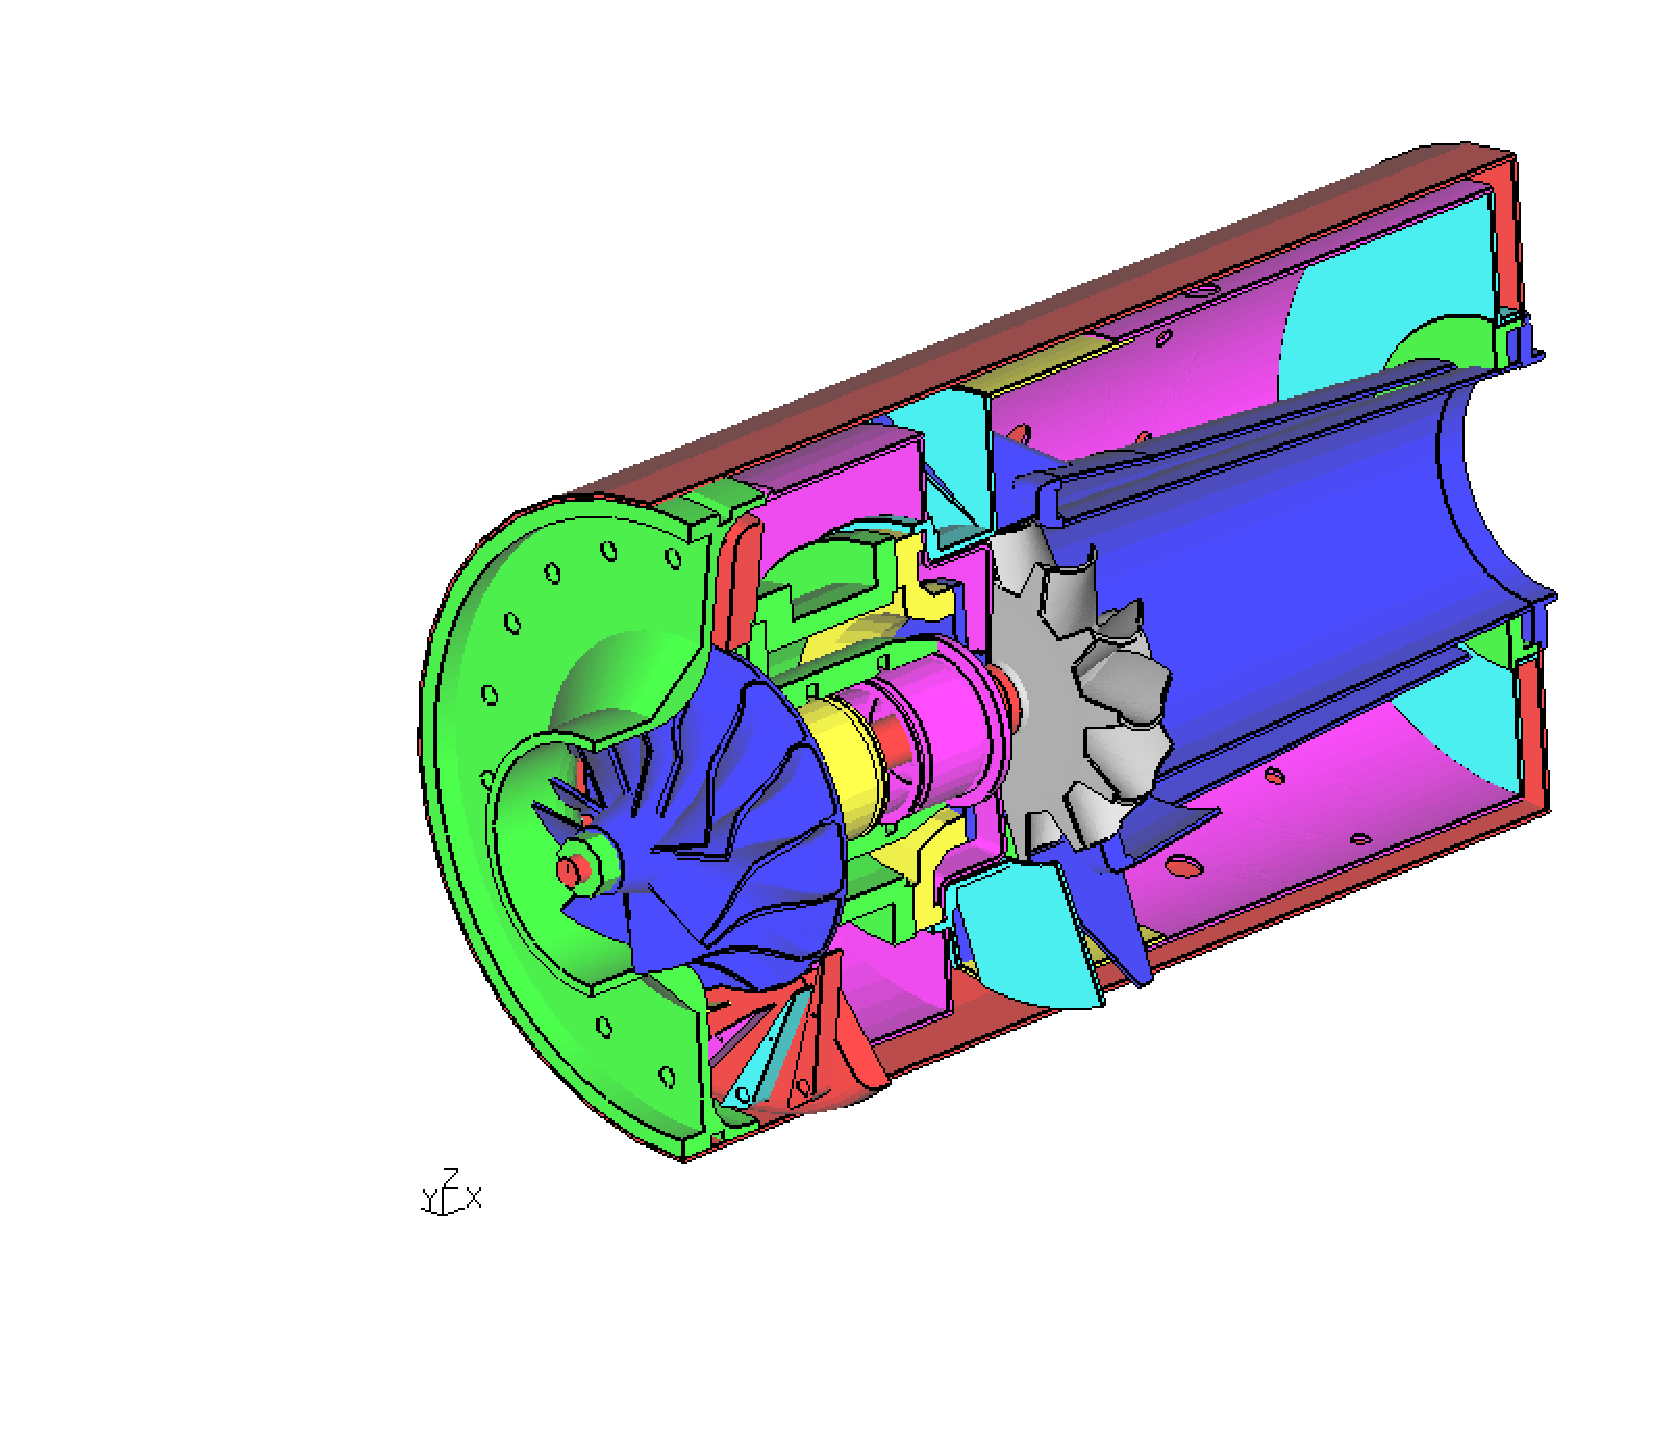
\epsfig{file=seta.eps,width=12cm}
\caption{\label{engine}All disjunct meshes in the jet-engine are successive coloured}
\end{figure}

\subsection{\label{setc}setc}
\begin{verbatim}
   'setc' [<set>] 
\end{verbatim}
This keyword is used to close an open set. Without parameter setc will close the at last opened set.

\subsection{\label{sete}sete}
\begin{verbatim}
   'sete' <set> 'n'|'e'|'p'|'l'|'c'|'s'|'b'|'S'|'L'|'se'|'sh' ->
                'max'|'min'|'strict'
\end{verbatim}
This keyword is used to enquire other sets which have entities in common or which have an identical content. Example:\\\\sete blade p min\\\\ searches for sets who store at least the same points as "blade" (always the set "all"). The option ``max'' searches for sets whose entities are completely included in the specified set. The option ``strict'' searches for identical sets regarding the specified type of entity.

\subsection{\label{seti}seti}
\begin{verbatim}
   'seti' <set> 'n'|'e'|'p'|'l'|'c'|'s'|'b'|'S'|'L'|'se'|'sh' ->
          <set> <set>.. 
\end{verbatim}
This keyword is used to generate an intersection of certain sets (what do the specified sets have in common of the specified entity-type?). Example:\\\\seti intersectSet p set1 set2 set3\\\\generates a set intersectSet with points which are stored in each of the sets set1 set2 set3.

\subsection{\label{seto}seto}
\begin{verbatim}
   'seto' [<set>] 
\end{verbatim}
This keyword is used to enquire open sets:\\\\
seto\\\\
Or to mark a set as open:\\\\
seto set\\\\
All newly defined or redefined entities will be members of all open sets. See \htmlref{setc}{setc} how to close an open set.

\subsection{\label{setr}setr}
\begin{verbatim}
   'setr' <set> 'n'|'e'|'p'|'l'|'s'|'b'|'L'|'S'|'v'|'se'|'sh'
                <name|*chars*> <name|*chars*> .. 
\end{verbatim}
This keyword is used to remove entities from a set (see also \htmlref{qrem}{qrem}. The entity will not be deleted. It is just not longer a member of that set. To remove entities from the set dummy type:\\\\setr dummy p p1 p2\\\\This will remove the points p1 and p2 from the set. The following entities are known: Nodes n, Elements e, Points p, Lines l, Surfaces s, Bodies b, Nurb Lines L, Nurb Surfaces S, Values v, other sets se and shapes sh. The program will automatically determine the type of the entities if not specified, but then the names must be unique. Wildcards (*) can be used to search for setnames of a certain expression.

\subsection{\label{shpe}shpe}
\begin{verbatim}
   'shpe' <name|!> ['pln' <P1> <P2> <P3>] |
                   ['cyl' <P1> <P2> <R1>] |
                   ['con' <P1> <P2> <R1> <R2>] |
                   ['sph'] <P1> <R1>]
\end{verbatim}
This keyword is used to create a shape which can be used to define the interiour of surfaces or to be used as a target for projections (see \htmlref{proj}{proj}) or to split entities (see \htmlref{split}{split}). A plane shape is defined with the parameter ``pln'' followed by the names of three points:\\\\shpe H001 pln P1 P2 P3\\\\A cylinder can be defined by\\\\shpe H001 cyl P1 P2 10.5\\\\were 10.5 is the radius. A cone can be defined by\\\\shpe H001 con P1 P2 10.5 2.\\\\were 10.5 is the radius at point P1 and 2. at point P2. A sphere can be defined by\\\\shpe H001 sph P1 10.5\\\\were 10.5 is the radius at point P1. If automatic name generation is desired, then use ''\verb_!_'' instead of a name. See also ``\htmlref{qshp}{qshp}'' for the mouse controlled definition of shapes.

\subsection{\label{split}split}
\begin{verbatim}
   'split' <set1> <set2> 
\end{verbatim}
This keyword is used to split lines, surfaces and elements.

The split command will not generate new surfaces but it will create points along the intersection between the surfaces in set1 and the surfaces (or shapes or faces) in set2.

So far only tetraeder elements (in set1) can be splitted by surfaces, faces or shapes (in set2). In this case the splitted tetraeder elements will be replaced by new tetraeder- and pentaeder elements. It can be used to cut out parts of the mesh to be either used directly in other models or which can be remeshed with tets based on an stl-file derived from them. Or it can be used to apply damages to a structure. See ``\htmlref{How to map loads}{How to map loads}'' in the appendix on how to map loads to the new created nodes from the original mesh.

\subsection{\label{stack}stack}
\begin{verbatim}
   'stack' on|off|free
\end{verbatim}
Several functions which return values to the user might now place them also on a software-stack (used by \htmlref{area}{area},\htmlref{dist}{dist},\htmlref{ds}{ds},\htmlref{enq}{enq},\htmlref{gtol}{gtol},\htmlref{length}{length},\htmlref{prnt}{prnt},\htmlref{valu}{valu},\htmlref{volu}{volu}). The ``\htmlref{valu}{valu}'' command is able to read this values from the stack and place them in variables. The 'free' parameter will empty the stack but does not open or close it.

See also ``\htmlref{if}{if}'' and ``\htmlref{while}{while}''.

\subsection{\label{steps}steps}
\begin{verbatim}
   'steps' <value> 
\end{verbatim}
This keyword is used to define the number of different colors in the post-processor mode. The default is 21.

\subsection{\label{surf}surf}
\begin{verbatim}
   'surf' <name(char<9)>|'!' [<set>]|->
               <line|lcmb> <line|lcmb> <line|lcmb> <line|lcmb>  
\end{verbatim}
This keyword is used to define or redefine a surface. It is a more convenient way to define a surface than the command \htmlref{gsur}{gsur}. Either individual lines or a set can be specified. To be meshable with structured elements it requires 3, 4 or 5 edges (lines or lcmbs). To be meshable with tr3u or tr6u it requires either to be plane or to reference a shape or nurbs which can not be provided with this command (see ``\htmlref{gsur}{gsur}. The most convenient way to define surfaces is to use the command \htmlref{qsur}{qsur}. 
If the name of the surface should be automatically generated, then just type ''\verb_!_'' instead of a name.

\subsection{\label{swep}swep}
\begin{verbatim}
  'swep' <set> <set> ['scal' <fx> <fy> <fz> <P0>|<div> [a] ]|
                     ['tra' <dx> <dy> <dz> <div> [a] ]|
                     ['rot' <p1> <p2> <alfa> <div> [a] ]|
                     ['rot' 'x'|'y'|'z' <alfa> <div> [a] ]|
                     ['rot' <p1> 'x'|'y'|'z' <alfa> <div> [a] ]|
                     ['rad' <p1> <p2> <dr> <div> [a] ]|
                     ['rad' 'x'|'y'|'z'|'p'<pnt> <dr> <div> [a] ]|
                     ['rad' <p1> 'x'|'y'|'z' <dr> <div> [a] ]|
                     ['mir' <P1> <P2> <div> [a] ]|
                     ['mir' 'x'|'y'|'z' <div> [a] ]|
                     ['mir' <P1> 'x'|'y'|'z' <div> [a] ] 
\end{verbatim}
This keyword is used to sweep entities into the next higher dimension. Sweeping a point will create a line, sweeping a line will create a surface and sweeping a surface will create a body. Shell elements will be expanded into Volume elements. The 'div' parameter defines how much elements will be created in the sweep direction. Existing results will be applied to the new nodes. Important: The ``\htmlref{trfm}{trfm}'' command must be used after the sweep operation and not before.

At first a copy of the first set (see \htmlref{seta}{seta} and \htmlref{copy}{copy}) will be created. The copy of the master-set is included in the second set. Then the connecting lines and surfaces are created and at last the bodies. The divisions of the new lines between set1 and set2 is specified with the parameter ''div'' or the default is used. Existing sets are extended by the copied entities if the last parameter ``a'' (append) is provided. Several transformations are available. For example scal creates a scaled copy, the scaling factors fx, fy, fz could be chosen independently,\\\\
swep part1 part2 scal 2 \\
swep part1 part2 scal 1 1 2 P0\\\\
tra will create a copy and will move it away by the vector dx, dy, dz and the optional parameter 'a' will assign the new entities to sets were the mother of each entity is included,\\\\
swep set1 set2 tra 10 20 30 a\\\\
rot will create a copy and will move it around the axis defined by the points p1 and p2 by 'alfa' degrees (the connecting lines will be of type arc below 180 deg, above a spline),\\\\
swep set1 set2 rot p0 px 20.\\\\
or the axis of rotation is given by specifying one of the basis coordinate axes:
swep set1 set2 rot x 20.\\\\
or just one point and a vector of rotation is given by specifying one of the basis coordinate axes:
swep set1 set2 rot p1 x 20.\\\\
rad will create a copy and uses the same transformation options as 'rot' or will create a spherical section if just a single point is defined,\\\\
swep sphere1 sphere2 rad pP0 10.\\\\
mir will create a mirrored copy. The mirror-plane is placed normal to the direction running from P1 to P2 and placed at P2,\\\\
swep section1 section2 mir p1 p2\\\\
as with 'rot and 'rad' additional transformation options are available:\\\\
swep section1 section2 mir P1 x\\\\
places the mirror at P1 with its normal direction in 'x' direction\\\\
swep section1 section2 mir x\\\\
Places the mirror in the origin with its normal direction in 'x' direction.

\subsection{\label{sys}sys}
\begin{verbatim}
   'sys' <shell-command parameters>
\end{verbatim}
This keyword is used to issue any shell command (unix or dos shell). For example to move files created by the 'send' command to certain file names or/and locations and to start the analysis. On certain platforms cgx will not wait for the completition of the command if the '\&' key was provided as the last argument of the command. Otherwhise cgx waits until the command was completed.

\subsection{\label{test}test}
\begin{verbatim}
   'test' 'v'|'n'|'e'|'p'|'l'|'c'|'s'|'b'|'S'|'L'|
          'se'|'sh' <entity> 
\end{verbatim}
Tests the existence of a given entity. Returns TRUE or FALSE and writes it on the stack.

\subsection{\label{text}text}
\begin{verbatim}
   'text' <string> 
\end{verbatim}
This keyword is used to define a comment. This commend will show up in the menu area of the main window below the file name. 

\subsection{\label{tra}tra}
\begin{verbatim}
   'tra' 'f'|'u'|'d'|'l'|'r' <relative-distance>
\end{verbatim}
This keyword is used to move the model in the window. For example\\\\tra u .1\\\\will move the model 0.1 times the model dimensions upwards. The meaning of the other letters is forward f, down d, right r, left l. 

\subsection{\label{trfm}trfm}
\begin{verbatim}
   'trfm' 'rec'|'cyl' ['x'|'y'|'z'] ->
        [<first-Dataset-Nr> [<last-Dataset-Nr>]]
\end{verbatim}
Changes dataset entities from one coordinate system to another. The option 'cyl' transforms the global results to cylindrical and 'rec' from cylindrical to global cartesian. In both cases the axis of the cylindrical system must be provided. Optionally the first and the last dataset of a range of a unique type can be specified. The current dataset is selected if no dataset is specified.

The transformation into the cylindrical system takes place in a way that tensors and vectors are transformed into a new local cartesian system which is alligned with the directions of a true cylindrical system. In this way the dimensions are maintained (for example the displacement in angular direction is not transformed into an angle but into a displacement in tangential direction).

The transformation from a cylindrical into a cartesian system works accordingly. Therefore successive "cyl" and "rec" commands are permitted. This command sequence can be used to rotate the model with its datasets in the correct way which means that all results are also rotated.

Example; Choose the desired dataset (and an entity) with the menu or the 'ds' command. Then type\\\\

trfm cyl z\\\\

to transform the dataset from a rectangular system into a cylindrical around the global z axis. Type\\\\

trfm rec z\\\\

to transform from cylindrical (which exists after the first call) to 
the rectangular system (which re-produces the original values).

To transform several datasets of the same type (!) at once:\\\\

trfm rec z 1 10000\\\\

This command transforms all datasets starting with the first to the last if the 
last dataset has a number below 10001 (but only the ones of the same type as 
the 1st!).


\subsection{\label{ucut}ucut}
\begin{verbatim}
   'ucut'
\end{verbatim}
If a section through the mesh was created with the "\htmlref{cut}{cut}" or "\htmlref{qcut}{qcut}" command then this command will delete the cut and display the un-cutted structure.

\subsection{\label{valu}valu}
\begin{verbatim}
   'valu' <name> [[<value>|'push'|'pop'] [nr]] | ->
         [['&'|'*'|'/'|'+'|'-'|'abs'|'max'|'min'|'pow'|->
          'sqr'|'sin'|'cos'|'tan'|'asin'|'acos'|'atan'] ->
          'int'|'float'|'exp' ->
         [name name] ]
\end{verbatim}
An entity which stores a string of characters. Most characters are valid but no white-spaces are accepted from the command line.
The command parser will scan each parameter of each command for expressions which match the name of a value and will replace the parameter by the content of the value. For example\\\\pnt P0 xvalue 0. 0.\\\\uses the value 'xvalue'. If the user has previously defined the value with:\\\\valu xvalue 1.24\\\\then the command-parser will replace 'xvalue' by '1.24' in the 'pnt' command.
\\\\ATTENTION: The commands 'prnt', all commands starting with 'set' except 'seta' and 'setr' and 'valu' itself are not parsed for substitution. To suppress the substitution the value has to be masked by a leading '\textbackslash{}'. For example the command:\\\\del v \textbackslash{}value\\\\will delete the value itself. The content of a value can be defined by the user\\\\valu arg1 1.24\\\\or derived from the stack previously filled by a command\\\\valu arg1 pop\\\\if the ''\htmlref{stack}{stack}'' was activated. A certain number on the stack can be addressed with\\\\valu arg1 pop 2\\\\were the '2' means that 2 successive 'pops' are executed. In this way the second value on the stack can be loaded at once.

Values can be written to the stack when the 'push' parameter is used:\\\\valu arg1 push\\\\A white-space separated string stored in a ``\htmlref{valu}{valu}'' will be written to the stack in separate sub-strings. With this method single pieces of a white-space separated string can be splitted and stored in separate values:\\\\stack on\\\\opens the stack\\\\valu complicatedString push\\\\splits the string stored in 'complicatedString' and writes the single pieces to the stack. The command \\\\valu subString pop 3\\\\loads the 3rd substring into the varible 'subString'.


The command is able to perform simple calculations like\\\\valu result * arg1 arg2\\\\'result' will store the product from 'arg1' and 'arg2'. It is important to understand that the command deals only with other 'values'. That means that a direct multiplication of two numbers is not possible. The number has to be stored in a value before it can be used:\\\\valu arg1 1.24\\\\assigns the string ``1.24'' to the value 'arg1'. During the calulation the strings are converted to double precision numbers and the result is stored as a string representing an exponential number. The 'int', 'float' and 'exp' convert between integer, floating point and exponential format.

The '\verb_&_' operator is used to concatenate two strings:\\\\valu string3 \verb_&_ string1 string2\\\\

See also ``\htmlref{prnt}{prnt}'' and ''\htmlref{How to write values to a file}{How to write values to a file}''.

\subsection{\label{view}view}
\begin{verbatim}
   'view' 'fill'|'line'|'point'|
          'edge' ['off']|'elem' ['off']|'surf'|'volu'|
          'front'|'back'|'vec' ['off']|'disp' ['off']|
          'bg' ['w'|'k']
\end{verbatim}
Commands to control the graphic output. This command is intended for batch-mode. See also ''\htmlref{Viewing}{Viewing}'' for the menu controlled functions.
\begin{itemize}
\item ''fill'' Element-faces are filled 
\item ''line'' Elements are displayed as fireframes
\item ''point'' Element-edges are displayed as points
\item ''edge'' triggers the display of the model edges were 
\item ''elem'' triggers the display of the element edges. They are deselected with the additional parameter ''off''.
\item ''surf'' and ''volu'' are used to display the structure either only by it's outer skin (surf) or by drawing all elements (volu). \item ''front'' and ''back'' define which side of the structure should be drawn. Either the side which faces the user or the back-side. If the back-side is displayed then internal structures are visible. 
\item ''vec'' triggers the vector mode. All vector-entities like displacements are displayed with arrows pointing in the direction of the vector and with a length proportional to the value of the vector. See ''\htmlref{Toggle Vector-Plot}{Toggle Vector-Plot}'' for a detailed description of the equivalent menu-function.
\item ''disp'' will show the deformed structure based on a formerly selected displacement dataset (no entity must be selected). See ''\htmlref{Toggle Add-Displacement}{Toggle Add-Displacement}'' for a detailed description of the equivalent menu-function.
\item ''bg'' Without second parameter toggles the background colour. The second parameter 'w' forces white while the parameter 'k' forces black as background colour.
\end{itemize}  

\subsection{\label{volu}volu}
\begin{verbatim}
   'volu' <set>
\end{verbatim}
This keyword is used to calculate the volume and the center of gravity of a set of volume-elements. If an ccx-input file with density data was read then the mass will be also calculated. If a 'dataset' is active then an averaged value is calculated.

The command writes to the ''\htmlref{stack}{stack}''.

\subsection{\label{while}while}
\begin{verbatim}
   'while' <value> 'eq'|'ne'|'=='|'!='|'<'|'>' <value>
\end{verbatim}
A command to compare two values. If the compare is True the following commands are executed until the 'endwhile' command is found. This procedure is repeated until the compare is False.
\\\\while arg1 == arg2\\\\will repeat the commands between 'while' and 'endwhile' until the nummerical value stored in 'arg1' is not equal to the nummerical value stored in value 'arg2'. The values are locally converted to 'float' format for the nummerical comparison. The 'eq' and 'ne' compare strings and should not be used for nummerical values since no conversion to a common format is done. Two strings are equal if they have the same length and all characters are equal.

See also ``\htmlref{if}{if}'', ``\htmlref{valu}{valu}'', ``\htmlref{stack}{stack}'' and ``\htmlref{How to run cgx in batch mode}{How to run cgx in batch mode}''.

\subsection{\label{zap}zap}
\begin{verbatim}
   'zap'  <set> 
\end{verbatim}
This keyword is used to delete all entities of a set and the set itself. All depending entities will be deleted as well.

\subsection{\label{zoom}zoom}
\begin{verbatim}
   'zoom' [<scale>]|[<p1x> <p1y> <p2x> <p2y>]
\end{verbatim}
This keyword is used to scale the model in the window. For example\\\\zoom 2\\\\will increase the size of the representation of the model by a factor of 2. A certain region of the model can be specified with two corner points of an imaginary rectangle. The coordinates are relative to the graphic-window which has its origin at the left/lower corner and as a fraction of the edge-lengths. For example \\\\zoom 0. 0. 0.5 0.5\\\\will display the third quadrant of the window scaled by a factor of 2.  

\newpage

\section{\label{Element Types}Element Types}
Node numbering of the elements and the type numbers used in the Result Format (frd-file). The solvers might use different node-numbering rules.

\begin{picture}(90,90)(0,150)
%
\put(0,0){\epsfig{file=be2.eps,width=9cm} }
\put(100,0){\label{topo_be2} 2 node beam element (be2, type 11) }
\end{picture}

\newpage

\begin{picture}(90,180)(0,330)
%
\put(0,360){\epsfig{file=be3.eps,width=9cm} }
\put(100,330){\label{topo_be3} 3 node beam element (be3, type 12) }
%
\put(0,30){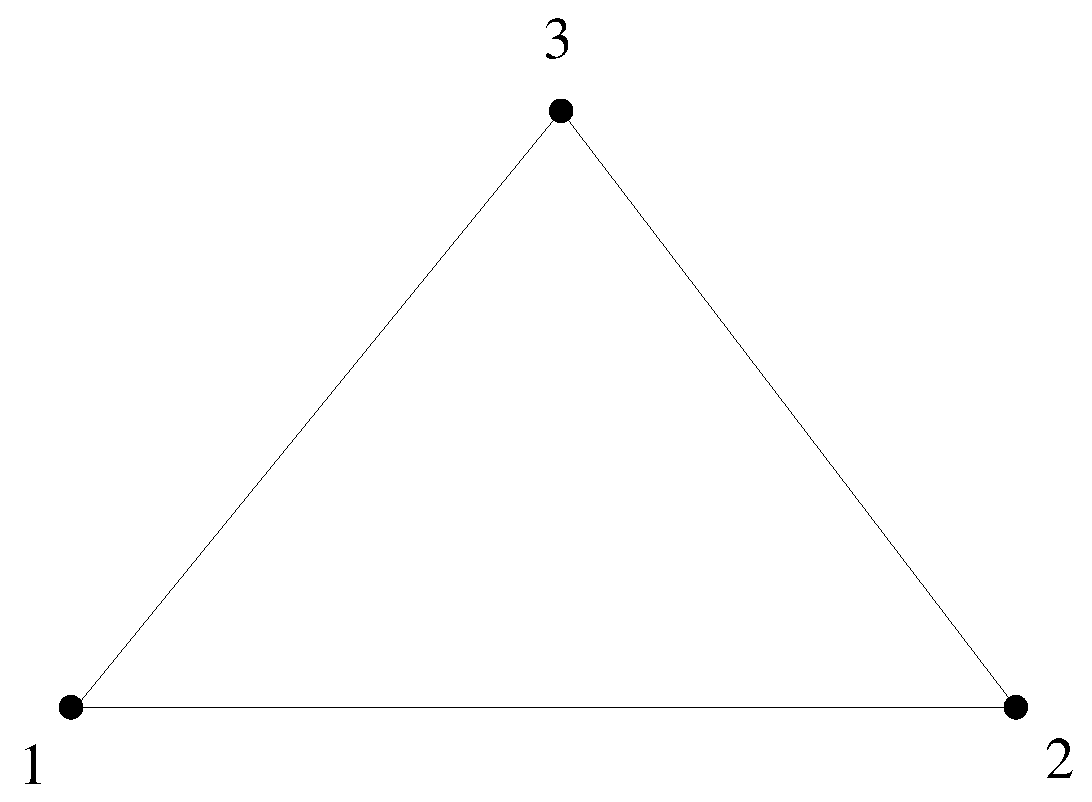
\epsfig{file=tr3.eps,width=10cm} }
\put(100,0){\label{topo_tr3} 3 node shell element (tr3, tr3u, type 7) }
\end{picture}

\newpage

\begin{picture}(90,180)(0,330)
%
\put(0,360){\epsfig{file=tr6.eps,width=10cm} }
\put(100,330){\label{topo_tr6} 6 node shell element (tr6, type 8) }
%
\put(0,30){\epsfig{file=qu4.eps,width=10cm} }
\put(100,0){\label{topo_qu4} 4 node shell element (qu4, type 9) }
\end{picture}

\newpage

\begin{picture}(90,180)(0,330)
%
\put(0,360){\epsfig{file=qu8.eps,width=10cm} }
\put(100,330){\label{topo_qu8} 8 node shell element (qu8, type 10) }
%
\put(0,30){\epsfig{file=te4.eps,width=10cm} }
\put(100,0){\label{topo_te4} 4 node tet element (type 3) }
\end{picture}

\newpage

\begin{picture}(90,180)(0,330)
%
\put(0,310){\epsfig{file=te10.eps,width=10cm} }
\put(100,280){\label{topo_te10} 10 node tet element (type 6) }
%
\put(0,30){\epsfig{file=he8.eps,width=10cm} }
\put(100,0){\label{topo_he8} 8 node brick element (he8, type 1) }
\end{picture}

\newpage

\begin{picture}(90,180)(0,330)
%
\put(0,360){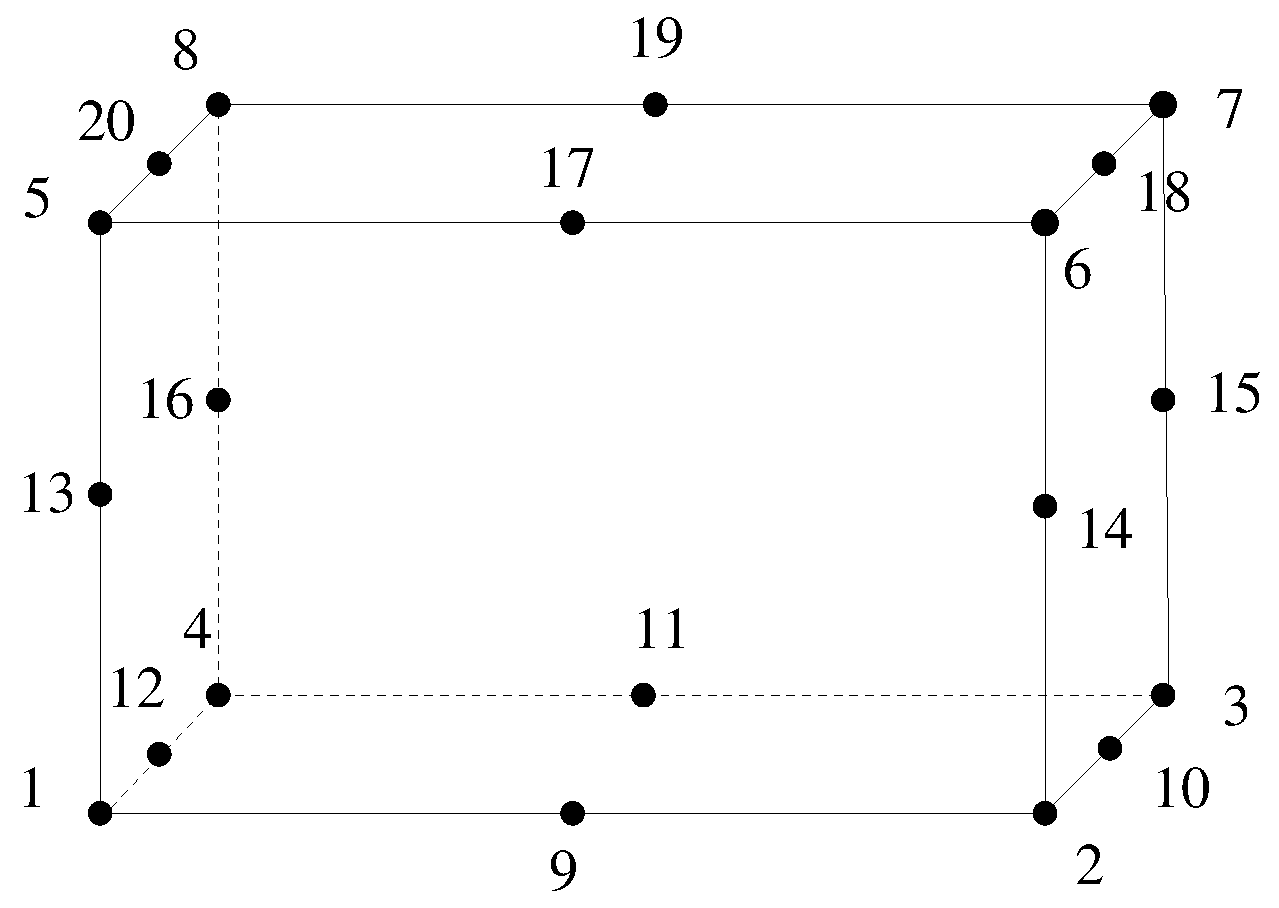
\epsfig{file=he20.eps,width=10cm} }
\put(100,330){\label{topo_he20} 20 node brick element (he20, type 4) }
%
\put(0,30){\epsfig{file=pe6.eps,width=6cm} }
\put(100,0){\label{topo_pe6} 6 node penta element (pe6, type 2) }
\end{picture}

\newpage

\begin{picture}(90,180)(0,330)
%
\put(0,360){\epsfig{file=pe15.eps,width=6cm} }
\put(100,330){\label{topo_pe15} 15 node penta element (pe15, type 5) }
\end{picture}

\section{\label{Result Format}Result Format}
Listing of the mesh- and the nodal results format. The data are stored in fixed format. Node-, element-definitions and results might be in ascii or binary coding. The ascii format is able to store element- and node-numbers up to '99999' in the short form or up to '9999999999' in the long form. An example for the short form is shown below:

\begin{verbatim}
>    1Ctest             !''1C'' defines a new calc of name ''test''
>    1UDATE  26.01.2000 !''1U'' stores user job-informations
>    2C                 !''2C'' starts a block of node coordinates
> -1    1 0.00000E+00 0.00000E+00 0.00000E+00 ! 1. node
> -1    2 0.10000E+01 0.00000E+00 0.00000E+00 ! 2. node ....
> -3                    !end of the current block
>    3C                 !''3C'' starts a block of elem definitions
> -1    1    4    0    0!first elem, type of that elem is 4 (he20)
> -2    1    2    3    4   13   14   15   16    5    6    7    8 ..
> -2   12   17   18   19   20 !twenty nodes defining that element
> -1 ...
> -2 ...
> -2 ...
> -3                    !end of the current block
>    1PHID      10      !defines a parameter HID value 10
>  100CL101            !''100C'' starts a user defined result block
> -4  DISP        3    1         !Attribute Header Record (Dataset)
> -5  D1          1    2    1    0 !Component Def. Record  (Entity)
> -5  D2          1    2    2    0
> -5  D3          1    2    3    0
> -1    1 0.00000E+00 1.00000E+00 1.00000E+00  !Nodal Values
> -1    2 1.00000E+00 0.00000E+00 0.00000E+00
> -3                      !end of the current block
> 9999                    !end of data
 
\end{verbatim}
The binary format applys only for data lines and the ``end of the current block'' line (-3), which is omitted.
All other lines are the same.

\subsection{\label{Model Header Record}Model Header Record}
\begin{verbatim}
Purpose: Defines the name of the model

Format:(1X,'   1','C',A6)  
Values: KEY, CODE, NAME
\end{verbatim}

\subsection{\label{User Header Record}User Header Record}
\begin{verbatim}
Purpose: Stores additional user informations regarding the job
         ie. user id, creation date, model informations

Format:(1X,'   1','U',A66)  
Values: KEY, CODE, STRING
\end{verbatim}

\subsection{\label{Nodal Point Coordinate Block}Nodal Point Coordinate Block}
\begin{verbatim}
Purpose: Defines the nodal coordinates

1. Record:
Format:(1X,'   2','C',18X,I12,37X,I1)
Values: KEY, CODE,NUMNOD, FORMAT
Where: KEY    = 2
       CODE   = C
       NUMNOD = Number of nodes in this block
       FORMAT = Format indicator
                0  short format
                1  long format 
                2  binary format, coordinates float 
                3  binary format, coordinates double 

Following records (ascci, FORMAT=0 | 1):
 Short Format:(1X,'-1',I5,3E12.5)
 Long Format:(1X,'-1',I10,3E12.5)
 Values: KEY, NODE, X,Y,Z
 Where: KEY    = -1
       NODE   = node number
       X..    = coordinates

Following records (binary, FORMAT=2):
 Format:(int NCOMPS*float)
 int and float are ansi-c data-types
 Values:  NODE, X,Y,Z
 Where: 
       NODE   = node number
       X..    = coordinates

Following records (binary, FORMAT=3):
 Format:(int NCOMPS*double)
 int and double are ansi-c data-types
 Values:  NODE, X,Y,Z
 Where: 
       NODE   = node number
       X..    = coordinates
  
Last Record (only FORMAT=0&1 (ascii), omitted for FORMAT=2&3):
Format:(1X,'-3')
Values: KEY
\end{verbatim}

\subsection{\label{Element Definition Block}Element Definition Block}
\begin{verbatim}
Purpose: Defines the topology of the elements

1. Record:
Format:(1X,'   3','C',18X,I12,37X,I1)
Values: KEY, CODE,NUMELEM, FORMAT
Where: KEY    = 3
       CODE   = C
       NUMELEM= Number of elements in this block
       FORMAT = Format indicator
                0  short format
                1  long format 
                2  binary format 

Following records (ascci, FORMAT=0 | 1):
 The following block of records must be repeated for each element:
  The first record initializes an element definition:
  Short Format:(1X,'-1',I5,3I5)
  Long Format:(1X,'-1',I10,3I5)
  Values: KEY, ELEMENT, TYPE, GROUP, MATERIAL
 Where: KEY    = -1
       NODE   = element number
       TYPE   = element type, see section ''Element Types''
       GROUP  = element group number, see command ''grps''
       MATERIAL= element material number, see command ''mats''.

  Then the nodes in the correct order have to follow:
  Short Format:(1X,'-2',15I5)
  Long Format:(1X,'-2',10I10)
  Values: KEY,NODE,NODE,NODE,NODE, ...
 Where: KEY    = -2
       NODE   = node number

Additional lines must follow if more nodes are used.

Following records (binary, FORMAT=2):
 Format:(4*int nodes*int)
 int and float are ansi-c data-types
 Values:  ELEMENT, TYPE, GROUP, MATERIAL,NODE,NODE,NODE,NODE, ...
 Where:
       ELEMENT= element number
       TYPE   = element type, see section ''Element Types''
       GROUP  = element group number, see command ''grps''
       MATERIAL= element material number, see command ''mats''.
       NODE   = node number
  
  
Last Record (only FORMAT=0 | 1 (ascii), omitted for FORMAT=2):
Format:(1X,'-3')
Values: KEY
\end{verbatim}

\subsection{\label{Parameter Header Record}Parameter Header Record}
\begin{verbatim}
Purpose: Stores informations related to datasets.
         ie. bondary conditions and loads
         They should consist of a keyword and a value

Format:(1X,'   1','P',A66)  
Values: KEY, CODE, STRING
Where: KEY    = 1
       CODE   = P
       STRING = Keyword Value (ie: FORCE 1000.)

\end{verbatim}

\subsection{\label{Nodal Results Block}Nodal Results Block}
\begin{verbatim}
Purpose: Stores values on node positions

1. Record:
Format:(1X,' 100','C',6A1,E12.5,I12,20A1,I2,I5,10A1,I2)
Values: KEY,CODE,SETNAME,VALUE,NUMNOD,TEXT,ICTYPE,NUMSTP,ANALYS,
        FORMAT
Where: KEY    = 100
       CODE   = C
       SETNAME= Name (not used)
       VALUE  = Could be frequency, time or any numerical value
       NUMNOD = Number of nodes in this nodal results block
       TEXT   = Any text
       ICTYPE = Analysis type
                0  static
                1  time step
                2  frequency
                3  load step
                4  user named
       NUMSTP = Step number
       ANALYS = Type of analysis (description)
       FORMAT = Format indicator
                0  short format
                1  long format 
                2  binary format 

2. Record:
Format:(1X,I2,2X,8A1,2I5)
Values: KEY, NAME, NCOMPS, IRTYPE
Where: KEY    = -4
       NAME   = Dataset name to be used in the menu
       NCOMPS = Number of entities
       IRTYPE = 1  Nodal data, material independent
                2  Nodal data, material dependant
                3  Element data at nodes (not used) 

3. Type of Record:
Format:(1X,I2,2X,8A1,5I5,8A1) 
Values: KEY, NAME, MENU, ICTYPE, ICIND1, ICIND2, IEXIST, ICNAME
Where: KEY    = -5
       NAME   = Entity name to be used in the menu for this comp.
       MENU   = 1
       ICTYPE = Type of entity
                1  scalar
                2  vector with 3 components
                4  matrix
               12  vector with 3 amplitudes and 3 phase-angles in
                   degree
               14  tensor with 6 amplitudes and 6 phase-angles in
                   degree
       ICIND1 = sub-component index or row number
       ICIND2 = column number for ICTYPE=4
       IEXIST = 0  data are provided
                1  data are to be calculated by predefined
                   functions (not used)
                2  as 0 but flaged by cgx
       ICNAME = Name of the predefined calculation (not used)
                ALL  calculate the total displacement if ICTYPE=2
This record must be repeated for each entity.

4. Type of Record:  (not used)
This record will be necessary in combination with the request for 
predefined calculations. This type of record is not allowed in
combination with binary coding of data.
Format:(1X,I2,2I5,20I3) 
Values: KEY,IRECTY,NUMCPS,(LSTCPS(I),I=1,NUMCPS)
Where: KEY    = -6
       IRECTY = Record variant identification number
       NUMCPS = Number of components
       LSTCPS = For each variant component, the position of the
                corresponding component in attribute definition


5. Type of Record:
The following records are data-records and the format is repeated
for each node.

In case of material independent data

- ascii coding:
Following records (ascci, FORMAT=0 | 1):
 Short Format:(1X,I2,I5,6E12.5)
 Long Format:(1X,I2,I10,6E12.5)
 Values: KEY, NODE, XX..
 Where: KEY  = -1 if its the first line of data for a given node
               -2 if its a continuation line
       NODE  = node number or blank if KEY=-2
       XX..  = data

- binary coding:
 Following records (ascci, FORMAT=2):
 (int,NCOMPS*float)
 int and float are ansi-c data-types
 Values: NODE, XX..
 Where:
       NODE   = node number or blank if KEY=-2
       XX..   = data

In case of material dependant data
REMARK: Implemented only for NMATS=1
- first line:
Short Format:(1X,I2,4I5)
Long Format:(1X,I2,I10,3I5)
Values: KEY, NODENR, NMATS
Where: KEY    = -1
       NODENR = Node number
       NMATS  = Number of different materials at this node(unused)
- second and following lines:
Short Format:(1X,I2,I5,6E12.5)
Long Format:(1X,I2,I10,6E12.5)
Values: KEY, MAT, XX, YY, ZZ, XY, YZ, ZX ..
Where: KEY    = -2 
       MAT    = material-property-number if KEY=-2 (unused)
       XX..   = data

  
Last Record (only FORMAT=0 | 1 (ascii), omitted for FORMAT=2):
Format:(1X,'-3')
Values: KEY

\end{verbatim}
 
\section{\label{Pre-defined Calculations}Pre-defined Calculations}
Listing of the automatically calculated additional results.

\subsection{\label{Von Mises Equivalent Stress}Von Mises Equivalent Stress}
Entity name: Mises\\
\[  \sigma_{vM} = \frac{1}{\sqrt{2}} \sqrt{(\sigma_{x}-\sigma_{y})^{2}+(\sigma_{y}-\sigma_{z})^{2}+(\sigma_{z}-\sigma_{x})^{2}+6\tau_{yz}^{2}+6\tau_{zx}^{2}+6\tau_{xy}^{2}} \]

\subsection{\label{Principal Stresses}Principal Stresses}
Entity names: P1, P2, P3, worstPS\\\\
The principal stresses $\sigma$ are named P1, P2, P3. From the three principal stresses $\sigma$ the absolute maximum value will be calculated and named worstPS. For example if a node has the three values 100, 0 and -110 MPa then -110 MPa would be shown. The three principal stresses $\sigma_{1}$ $\sigma_{2}$ $\sigma_{3}$ are derived from the following equation:
\[
\left [
\begin{array}{ccc}
\sigma_{xx}-\lambda & \sigma_{xy} & \sigma_{xz}\\
\sigma_{yx} & \sigma_{yy}-\lambda & \sigma_{yz}\\
\sigma_{zx} & \sigma_{zy} & \sigma_{zz}-\lambda
\end{array}
\right ]
\left [
\begin{array}{c}
nx\\
ny\\
nz
\end{array}
\right ]
= 
\left [
\begin{array}{c}
0\\
0\\
0
\end{array}
\right ]
\]
They are given by the three roots of the equation (stress tensor is symmetric: $\sigma_{xy}$ = $\sigma_{yx}$ etc.):
\[ \sigma^3 - (\sigma_{xx}+\sigma_{yy}+\sigma_{zz})\sigma^2 + (\sigma_{xx}\sigma_{yy}+\sigma_{yy}\sigma_{zz}+\sigma_{zz}\sigma_{xx}-\sigma_{xy}^2-\sigma_{yz}^2-\]\[\sigma_{zx}^2)\sigma - (\sigma_{xx}\sigma_{yy}\sigma_{zz}+2\sigma_{xy}\sigma_{yz}\sigma_{zx}-\sigma_{xx}\sigma_{yz}^2-\sigma_{yy}\sigma_{zx}^2-\sigma_{zz}\sigma_{xy}^2)  = 0 \]

\subsection{\label{maxShear Stress}maxShear Stresses}
Entity name: maxShear\\
This is the maximum shear-stress:
\[ maxShear = 0.5 * (\sigma_{1} - \sigma_{3}) \]

\subsection{\label{Cylindrical Stresses}Cylindrical Stresses}
Entity names: SXX, STT, SRR, SXT, STR, SRX\\\\
The Cylindrical Stresses are truly cartesin stresses in a cylindrical system regarding the node-position relative to the axis of the cylindrical system. The stress-tensor is rotated individually for each node. They are calculated on demand (see \htmlref{trfm}{trfm}).

 \section{\label{Meshing rules}Meshing rules}
Some rules must be fulfilled before a geometry is meshable (see \htmlref{mesh}{mesh}). For linear elements (ie. qu4 or he8), the sum of all divisions (see \htmlref{div}{div}) of each surface must be even. In case of quadratic elements (ie. qu8 or he20) this sum must be divisible by 4 without residue. Opposite edges of a given surface might have different divisions. For example on the left side of a given surface the division is 8 and on the right side it is only 4. But only two opposite surfaces of a body can use this feature. These surfaces are called top and bottom surfaces. All other surfaces of this body must have unique divisions on opposite edges. In case of 3 sided surfaces it is necessary to apply a minimum division sufficient for two elements along the edge. The only exception is the element tr3u (see \htmlref{elty}{elty}) which allows a division of one.

A body can not be meshed when the shape of the body is very far from being brick-like. The body might be subdivided to improve the shapes of the single ones. There is a restriction for the definition of five- or seven-sided bodies. The first two surfaces in the body-topology (see \htmlref{gbod}{gbod}) have to be defined in the same order. That means the first line of the first surface has to be connected with the first line in the second surface by one of the remaining surfaces. This is always the case if the body is a product of a ''\htmlref{swep}{swep}'' command.

 \section{\label{User-Functions}User-Functions}
The user might define his own functions to manipulate the mesh or the results with the user function stored in file ''userFunction.c''. See the command ''\htmlref{call}{call}'' how to call a user function. The user can generate new nodes, elements or datasets or extend or manipulate existing datasets or interfaces to other software. The file ''userFunction.c'' includes an example which calculates the hydrostatic stress and stores the result in a new dataset. There the user can see how to deal with datasets.

\begin{appendix}
\section{\label{Known Problems}Known Problems}
\subsection{\label{Program is not responding}Program is not responding}
If the program seems to hang then leave the window with the mouse pointer and go in again. If that does not help then probably a command is waiting for input. Stay with the mouse pointer inside the window and press the ''q'' key several times. Another very popular error is to move the mouse-pointer into the xterm were the typed commands and the protocol is visible. Please, the mouse-pointer MUST stay in the main-window during typing! 

\subsection{\label{Program generates a segmentation fault}Program generates a segmentation fault}
Write a mail to the author and, if possible, add the input-file.\cite{cgx}.

\section{\label{Tips and Hints}Tips and Hints}
The following collection will give you background information and procedures to deal with common situations.

\subsection{\label{How to change the format of the movie file}How to change the format of the movie file}
Use a shell command like convert to split up movie.gif with multiple
layers into multiple frames, as seperate jpeg files:
\begin{verbatim}
convert movie.gif %d.jpg
\end{verbatim}
Convert any series of multiple jpeg files into WMV format with:
\begin{verbatim}
mencoder 'mf://*.jpg' -mf type=jpg:fps=25 -ovc lavc -lavcopts
vcodec=wmv2 -o movie.wmv
\end{verbatim}
To convert a video file into avi format use this command:
\begin{verbatim}
mencoder <videofile> -ovc lavc -lavcopts vcodec=flv -of avi -o movie.avi
\end{verbatim}
In general:To convert a video file from one format into the other, use
the program "mencoder". It comes with the mplayer packages. 
\begin{verbatim}
mplayer movie.wmv
\end{verbatim}


\subsection{\label{How to define a set of entities}How to define a set of entities}
Some knowledge is necessary to efficiently select entities (nodes, points ..). As a golden rule in complicated situations never try to create a set just by ''adding'' the entities to the set (see \htmlref{qadd}{qadd}). It is much better to catch a bigger group which includes certainly the wanted ones. Then display the set with the \htmlref{plot}{plot} command and remove all unwanted entities with the \htmlref{qrem}{qrem} command. Entities are selected if at least one pixel of it is inside the selection rectangle. But there is one exception: Only the lower left corner of any text (names of points etc.) can be selected. Surfaces can also be selected by picking its shaded interiour (see ``\htmlref{rep}{rep})''. You might add all lower entities (as points for example) by typing ''\htmlref{comp}{comp} set do''. This is necessary for example if you had selected surfaces and you want to move them in space. Only points have locations and therefore nothing will happen unless you completed the set by the related points with ''comp'' command.

There is another type of set called sequence. The data-structure is the same but with one exception, the data keep their order in which they were selected. This type of set is used for splines (see ''\htmlref{qlin}{qlin}'' and ''\htmlref{line}{line}'') or in combination with the ''\htmlref{graph}{graph}'' command if values along a path should be displayed. Use ''\htmlref{prnt}{prnt} sq'' to list all existing sequences and use ''\htmlref{qseq}{qseq}'' or ''\htmlref{seqa}{seqa}'' to create them. Up to now they are only used to store nodes and points. As sets they will be written to a file if fbd format is specified. In this case also node-sequences can be stored.

\subsection{\label{How to enquire node numbers and values at certain locations}How to enquire node numbers and values at certain locations}
A very common problem is how to get the exact value on a node position during post-processing. To actually get the value add the element edges to the view (see \htmlref{Toggle Element Edges}{Toggle Element Edges}) and type \htmlref{qenq}{qenq} and press the RETURN key (during typing the mouse-pointer MUST stay in the main window, do NOT move the pointer into the xterm). Then move the mouse-pointer over the location of a node and press the ''n'' key. The node-number, the value at that node and the location will be written in the xterm from which the cgx was started. See also the ''\htmlref{enq}{enq}'' command for batch controlled value extraction.

\subsection{\label{How to write values to a file}How to write values to a file}
When you need to write certain values (see ``\htmlref{valu}{valu}'') to a file you may use the 'echo' system command:
\begin{itemize}
\item Choose the relevant dataset (menu or ds command)
\item Add the relevant nodes to a set (qadd setname or seta setname n ..) 
\item Open the stack: stack on
\item Place node-values on the stack: prnt se setname
\item Store the node: valu nod1 pop 
\item Store the value: valu val1 pop 
\item Write to file: sys echo Node nod1 Value val1 \verb_>|_ file.txt
\end{itemize}
See also ``\htmlref{if}{if}'' and ``\htmlref{while}{while}'' and see the demo in ``\htmlref{If and while demo}{If and while demo}'' on how to work with this commands. They are usefull for automatic post-processing.

\subsection{\label{How to select only nodes on the surface}How to select only nodes on the surface}
Some times you need to select nodes only on the surface of the mesh. This can be done when the mesh is displayed in the surface mode (see ''\htmlref{Toggle Surfaces/Volumes}{Toggle Surfaces/Volumes}'') using the menu-entry ''\htmlref{Show Elements With Light}{Show Elements With Light}''. To find node positions more easily add the element edges to the view (see \htmlref{Toggle Element Edges}{Toggle Element Edges}).

A different way uses the element-faces (see ''\htmlref{plot}{plot}'' with parameter ''f''). Store the desired faces in a new set (\htmlref{qadd}{qadd}) and complete the set downwards (``\htmlref{comp}{comp} set do''). Check the selected nodes with ``plot n setname''. 

\subsection{\label{How to generate a time-history plot}How to generate a time-history plot}
So called time history plots can be created based on a previous displayed sequence of data-sets (see ''\htmlref{Toggle Dataset Sequence}{Toggle Dataset Sequence}'') with the command ''\htmlref{graph}{graph}''. It is also possible to use only the command line. For example:
\begin{itemize}
\item ds 1 e 3
\item ds 1 2 10
\item graph set t
\end{itemize}
will produce a time history plot for the nodes stored in set over all loadcases from 1 to 10 for the entity nr 3.
Or
\begin{itemize}
\item graph set t DISP D1
\end{itemize}
will display the displacement in direction 1 for all loadcases.
For more details and other options look into the ''\htmlref{graph}{graph}'' command description.
\newpage

\begin{figure}[h]
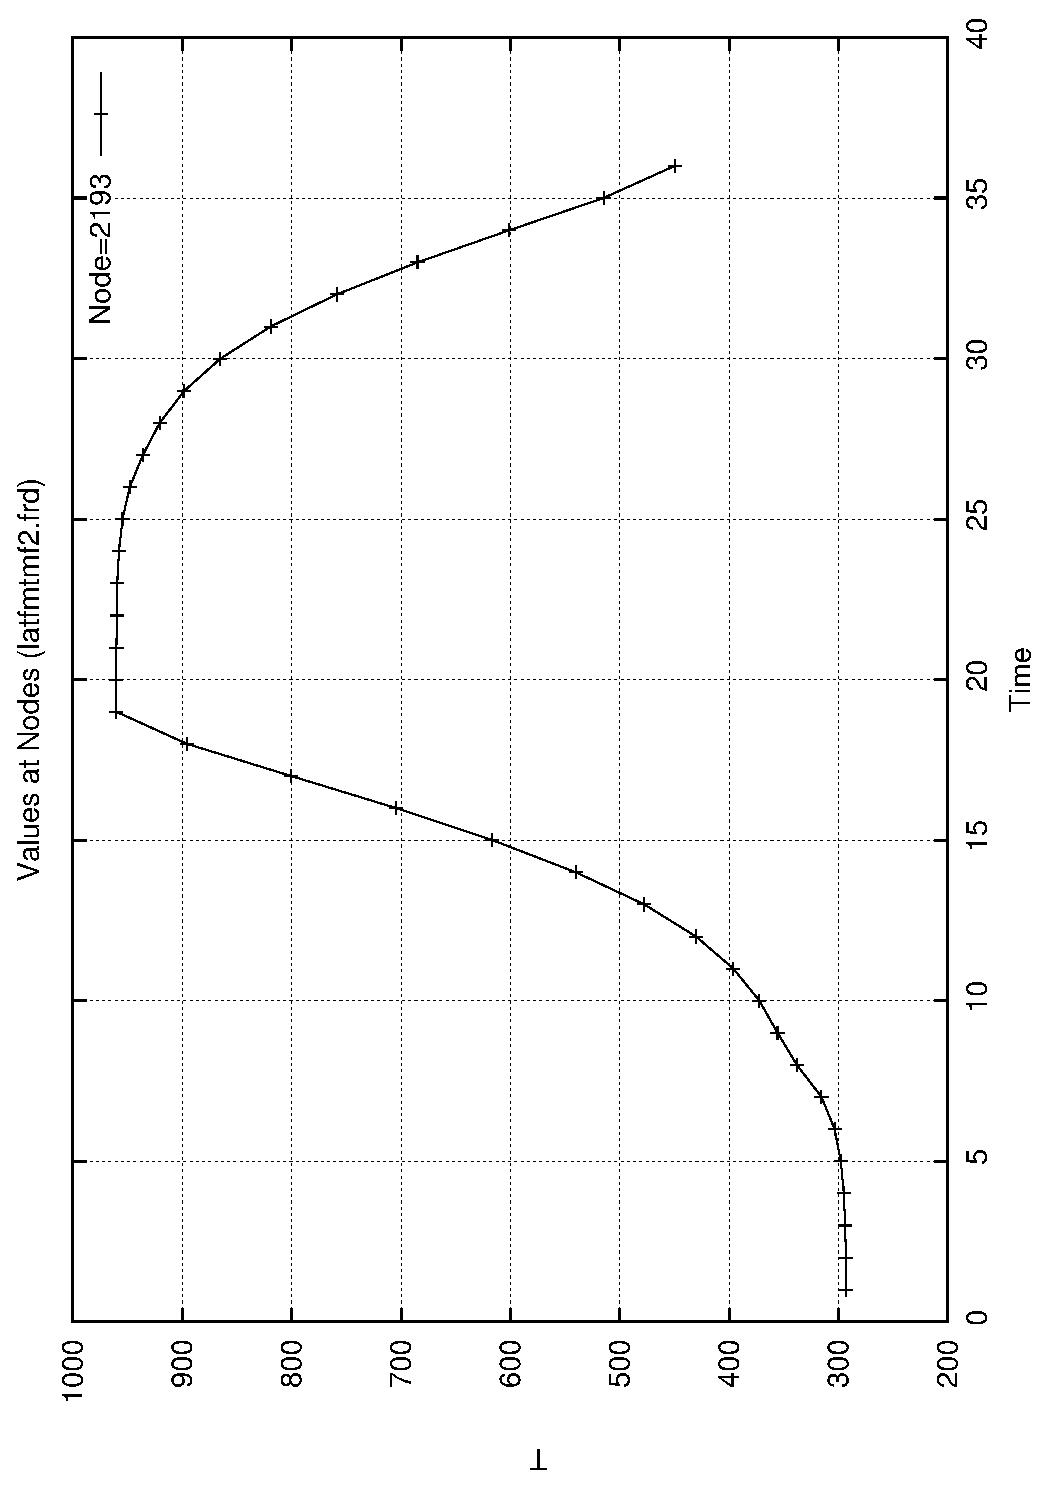
\epsfig{file=graph.eps,width=9cm}
\caption{\label{graph2D} example of a time-history plot }
\end{figure}


\subsection{\label{How the mesh is related to the geometry}How the mesh is related to the geometry}
Very often you need the embedded nodes, element-faces or elements of geometric entities to apply boundary conditions. If you understand the underlying concept you will be able to get them more easily.

Geometric entities are the mothers of nodes, faces and elements (so to say) and will remember them. In turn if an entity is not the mother of a given mesh-entity it will not remember it. Therefore a body will only know about nodes which are not placed on surfaces, lines or points. A surface will only know about nodes which are not placed on lines or points. And so on.

Therefore if you need the nodes on a surface and not only the ones just inside the surface, then create a set with this surface and do a ''\htmlref{comp}{comp} set do''. This will add the lines and points together with their nodes to the set.

On the other hand if you have only a node and you need the geometric entity in which the node is embedded you might also type ''comp set do''.


\subsection{\label{How to change the order of elements}How to change the order of elements}
Use the command ''\htmlref{mids}{mids}'' to change from second order to first order or vice versa. In this case the amount of elements will not change. Or use the command ''\htmlref{send}{send}'' with the parameter ``quadlin'' to change from second order to first order. But in this case each second order element will be splitted in 8 first order elements. 


\subsection{\label{How to connect independent meshes}How to connect independent meshes}
Sometimes it is advisable to ''glue'' independent meshes together instead of trying to create one big seamless-mesh. Or you just want to create a contact formulation were you know that no separation will happen. In this situations you might use equations (also called mpc's) which connect one dependent node with one or more independent nodes. The independent side should be coarser than the dependent side to avoid gaps in the connection. See the command ''\htmlref{send}{send} in combination with the option ''areampc'' how to create such connections. Sliding and fixed contact as well as press-fits can be modelled. The necessary sets should be defined based on geometry not on the mesh. In this case the definition will be stored with the ''save'' or ''exit'' command and can be used after the next program call.

Background: The movement of each location in an element (or on its surface) is fully described by the movement of its associated nodes and its shape-function. In an iterative algorithm element-coordinates are varied until the real-world coordinates of a dependent node are matched. Based on the element coordinates the shape function gives the participation (weight) factors of the independent nodes (the coefficients in the mpc's). This approach delivers valid results as long as the dependent node is not located outside of the independent element. Therefore the location of the dependent node has to be modified in such cases. The dependent will be moved to the surface of the independent element (again decribed by its shape-function) and the procedure is repeated.

\begin{figure}[h]
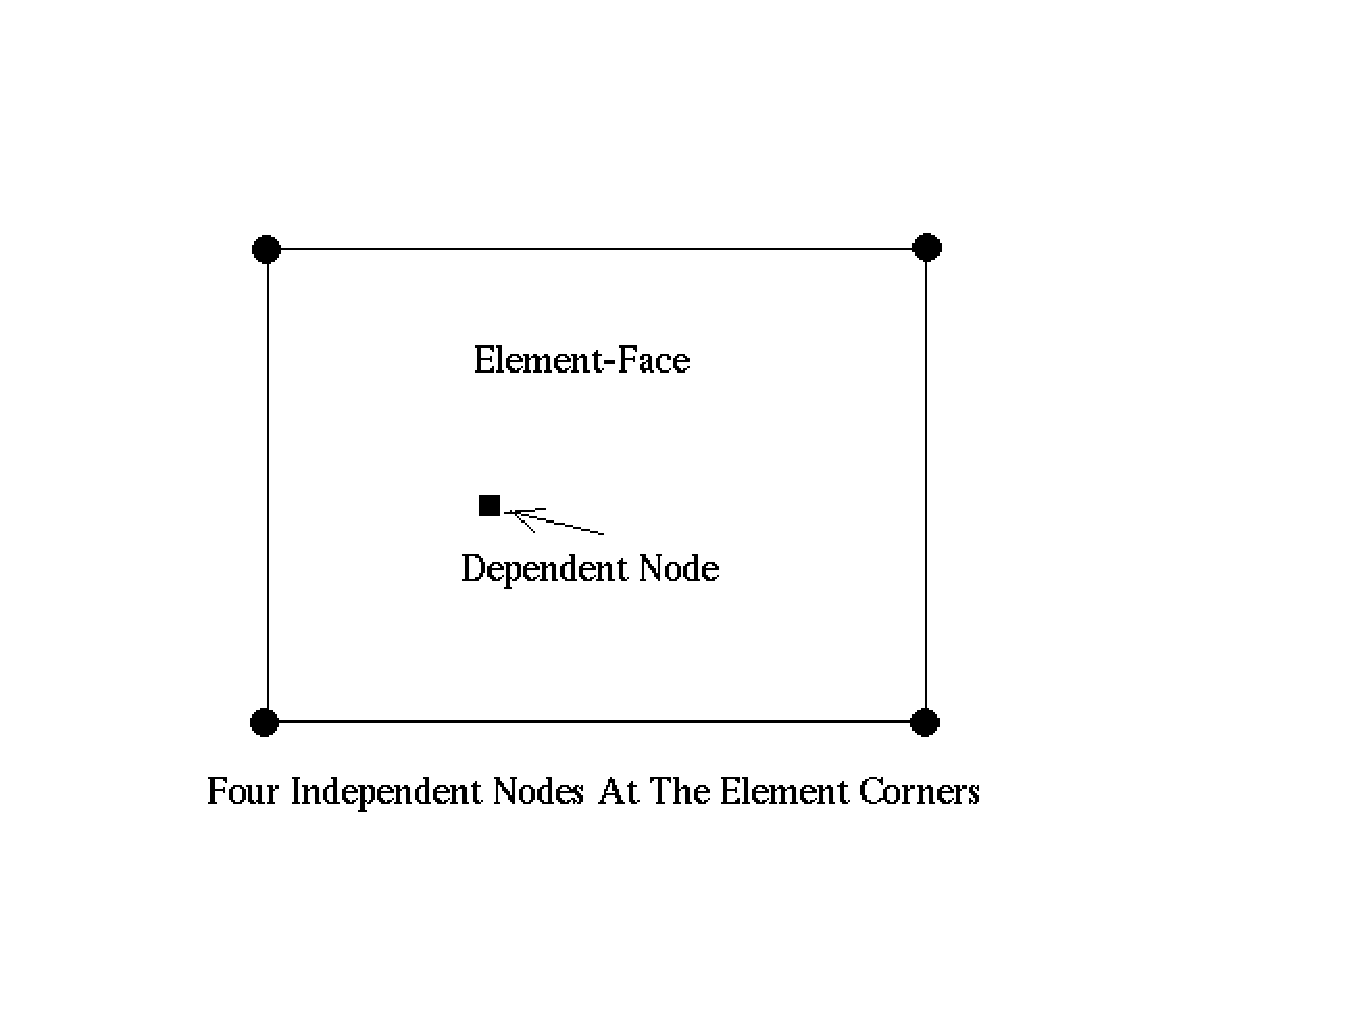
\epsfig{file=equation.eps,width=12cm}
\caption{\label{equation} Dependent node on element face to create a connection  }
\end{figure}


\subsection{\label{How to define loads and constraints}How to define loads and constraints}
Loads and constraints are not saved in any database. They are just created and written to a file with the ''\htmlref{send}{send}'' command. But the sets which are needed for the definition are stored together with the geometry if you type the ''\htmlref{save}{save}'' command. Of course the sets must have been defined based on geometry and not based on mesh entities like nodes because mesh-entities are not saved with the ''save'' command. You must know that geometry-sets know also their mesh entities after a ''\htmlref{mesh}{mesh}'' command.
If you store your commands to write the boundary conditions in a file you can easily repeat them by just reading this command-file (see ''\htmlref{read}{read}''). Several types of loads can be applied. That is forces, pressure, thermal-heat-coefficients and radiation etc. For unsupported loads write a set of element-, node- or face-labels (parameter ''names'') and apply the desired load to that set in the solver input-file. Other boundary conditions like single-point-constraints for structural, thermal and fluid-calculations can be written. The sliding condition (parameter ''slide'') were nodes are bound to the element-faces to which they belong can be used for structural calculations or for fluid calculations. In the later case it forces the flow to follow the surface of the elements. This is necessary in inviscid calculations to prevent the fluid to penetrate the walls. Results from a previous calculation can be written in the solver input format for further calculations (parameter ''ds'', ''tmf'' etc.). For example temperatures for thermal mechanic fatigue analysis or velocities, pressures and thermals for a restart of a cfd calculation.


\subsection{\label{How to map loads}How to map loads}
Values at nodes can be mapped (interpolated) from a second mesh with the ''\htmlref{map}{map}'' command. This second mesh (data source or ``master'') is usually available as a result-file from a previous calculation. The ''\htmlref{read}{read}'' command with the ``add'' parameter can be used to include this file in the current model. Solver-input files (inp) and result files (frd) can be used as a data source. The command will add an offset to the nodes and elements so that existing nodes and elements will not be overwritten. The original mesh is the target or ``slave'' of the mapping process. The mapping process will add the values to the dataset(s). The mapped values can be visualized by selecting the mapped dataset and entity and then by plotting the slave elements or faces with ``\htmlref{plot}{plot} fv slave''. An example of the necessary commands for the mapping process (2D to 2D) is listed below:
\begin{verbatim}
  Define a set with the slave nodes or faces. For example with:
    qadd slave
    comp slave do (to extend the set by the referenced faces or
                   nodes)

  Then open a set and read the master-model:
    seto new
    read result.frd add
    setc

  If necessary move 'new' in space to match the position of the
  slave (see ``move'').

  Add the faces to the 'new' set
  (only nodes and elements are already stored in "new"):
    comp new do
    plot f new

  Define the master set:
    qadd master  (catch the right faces)
    comp master do

  Map the values of dataset 1 with:
    map slave master surf ds1

  Check the mapping with:
    ds 1 e 1
    plot fv slave

  Write the file with the mapped values:
    send slave abq pres ds1 e1

  Check the file ``slave_ds1e1.dlo'' with an editor and use it
  in an inp-file.
\end{verbatim}
If the master values are not available in either inp or frd format but in any other format which can be read by cgx (isaac, openFoam ..) it is then possible to write them in frd format with the ''\htmlref{send}{send}'' command.


\subsection{\label{How to run cgx in batch mode}How to run cgx in batch mode}
Most commands can be executed in batch-mode. Actually if you read a file with geometry (fbd-file) then you run cgx in batch mode already! You just have to add ''exit'' or ''quit'' at the end of the file and it will be obvious. You might use the ''\htmlref{read}{read}'' command in such a command-file to reference other command-files or to read files with mesh-entities for whatever purposes. In such a way you can create and modify geometry or meshes in batch-mode or evaluate results in batch-mode. But you need a graphic-capable computer because cgx needs it also if no graphic output is requested. Nevertheless the popup of the graphic window can be suppressed if cgx was started with the ``-bg'' parameter.

Some commands make only sense in a batch file like ``\htmlref{if}{if}'' and ``\htmlref{while}{while}''. Please see also the demo in ``\htmlref{If and while demo}{If and while demo}'' on how to work with this commands. See also ``\htmlref{How to write values to a file}{How to write values to a file}''.

It should be noted that a successive 'save' or 'exit' command will overwrite the batch file if it has the file-extension 'fbd'. To prevent this the user should use a different extension like 'fbl'.

\subsection{\label{How to deal with cad-geometry}How to deal with cad-geometry}
In general hexahedra-elements perform better than tets but if the mesh should be derived from a cad-geometry it is often more convenient to create a tetrahedra mesh as to modify or rebuild the geometry to make it meshable with hexahedra-elements. The following section gives some hints which alternatives are available.

\begin{itemize}
\item A simple step-reader is integrated in cgx (cgx -step filename). It can deal with points and lines. This is sufficient to create simple hexaeder elements for axis-symmetric structures like a rotor but the experienced user might use the following approach also for more complex geometries. You might start with a file containing a 2D-section, subdivide it in mesh-able surfaces and sweep it in the 3rd dimension to create your geometry (see \htmlref{swep}{swep}). If features exist in the 3rd dimension then this features must be included in the 2D-section. Then sweep the 2D-section to the location were the feature starts, then right to the end and at last to the end of the geometry. Then delete the unwanted bodies before and after the feature. You might also project the sweped sections to target surfaces if the feature is shaped in the 3rd dimension (see \htmlref{proj}{proj}).

Sometimes the geometry consists of several parts which are arranged on different positions in space. This is called assembly. When cgx is started with the parameter ``-stepsplit'' instead of ``-step'' it will write the single parts to separate directories using their original coordinate systems. The user can prepare meshable geometry or meshes based on them. But he must use the filenames which he finds there. The final meshed assembly can be build afterwards by calling the fbl-file which was written by cgx. This fbl-file contains the original step-commands to position and eventually duplicate the single geometries/meshes from the subdirectories.   

\item For CAD models in STEP- or IGES-format you should consider to use a tet-mesher like NETGEN \cite{NETGEN} which generates quite nice tet-meshes. You can read this meshes with cgx and combine them with cgx-geometry and meshes. Then create your boundary conditions etc. You might read the native-netgen format (.vol) instead of abaqus-format because this includes the 2D meshing regions as separate sets which can be used to apply boundary conditions (``cgx -ng file.vol''). See the ''\htmlref{Program Parameters}{Program Parameters}'' section on how to do that.

\item The CAD-model is available in VDA-format. In this case the user can mesh the surfaces with structured- \cite{Coons} (elty setname tr3 etc.) or unstructured triangles \cite{mesh2d} (elty setname tr3u etc.) and use them to be replaced by tets created by an external auto-mesher called from within cgx. The cgx uses the tet-mesher from NETGEN \cite{NETGEN} for this task. 
\end{itemize}

Therefore cgx can only generate a tet-mesh if NETGEN is installed and the program ng\_vol (part of NETGEN) is accessible. For the full functionallity replace the original ng\_vol in the NETGEN package with the modified program ng\_vol from the cgx-distribution and build it again.

The following section describes the process to generate a tet-mesh with cgx based on a cad model in VDA-file format:


\begin{figure}[h]
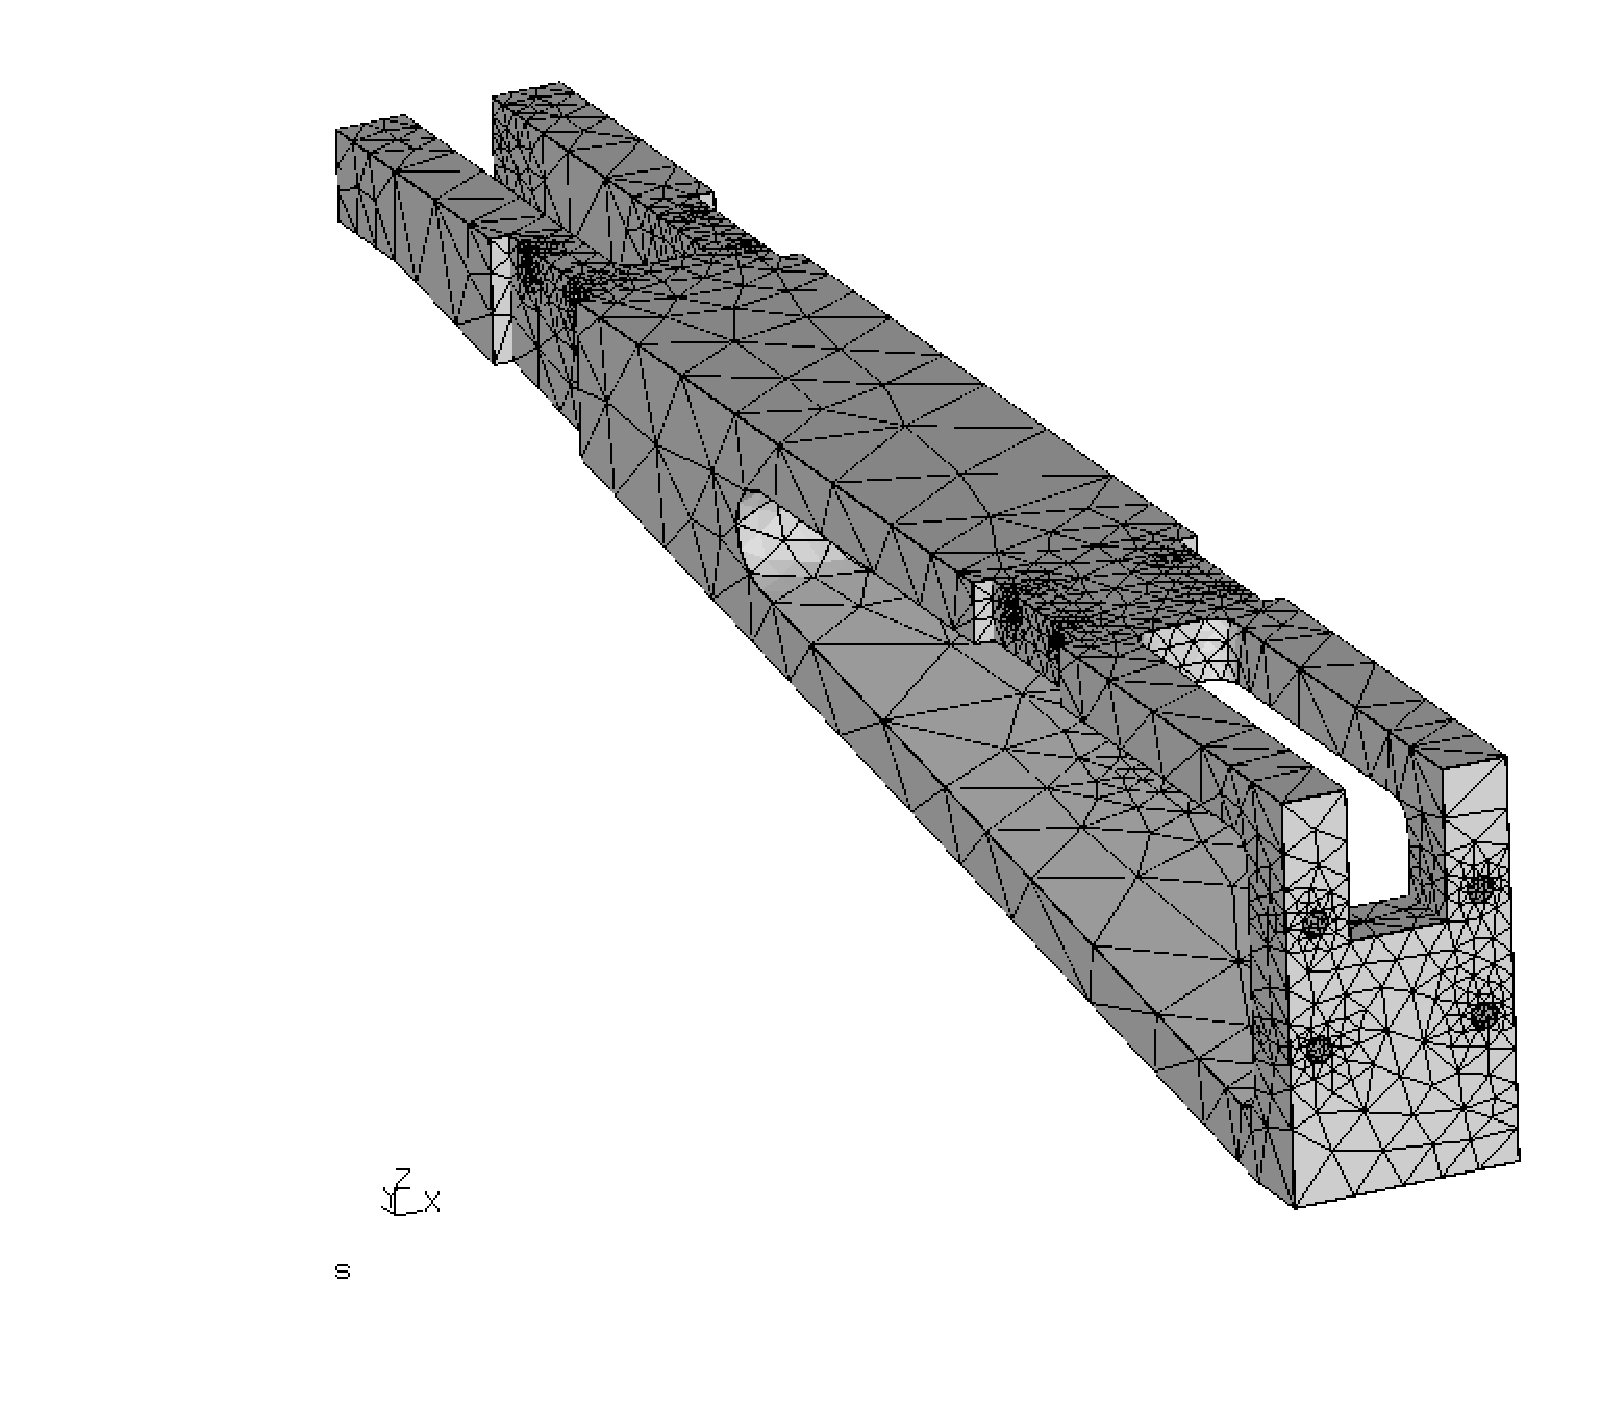
\epsfig{file=halter.eps,width=9cm}
\caption{\label{halter} CAD-geometry meshed with tet-elements }
\end{figure}

\begin{itemize}

\item Use the interface program to convert the cad format to fbd format (You find example data (vda) in CalculiX/cgx\_2.7/examples/cad)\begin{verbatim} (ie: vda2fbd halter.vda > halter.fbd). \end{verbatim} In some cases the header of the vda file causes trouble and must be modified to make the program run.

\item Start cgx with that file (cgx -a halter.fbd). Usually some warnings appear on the screen but the program will fix that automatically (triggered by the parameter -a). After all geometry has been read the program will merge points and lines to close the volume. Then all nurbs related surfaces might be trimmed (optional). This has to be done manually by typing ``rep all''. Finally, with the command ``plus si all'' all surfaces are rendered and the result is displayed in the main window. The whole process might need some time. If problems occur the user might start the program with option -b instead of -a (cgx -b halter.fbd). Then no automatic post-processing is done and the user has to prepare the geometry manually. See the commands \htmlref{merg}{merg}, \htmlref{div}{div}, \htmlref{qdiv}{qdiv}, \htmlref{qlin}{qlin}, \htmlref{rep}{rep}.

\item If a surface points inwards it is not illuminated and appears only dark grey. Flip the surfaces in a way that its normal direction points outwards (use ''\htmlref{qflp}{qflp}''. Press the ''a'' key to selet the ``all'' mode and then select a correctly oriented surface by pressing key ''s'', all other surfaces will immediatelly use the same orientation).

\item Define the element type (see \htmlref{elty}{elty}). In most cases it is advisable to use triangles first and not directly tetraeders because this has the advantage that the surface mesh can interactively improved before the tets are generated. Remark: If you choose tets from the beginning, you must first create a body with ``body ! all'' before you can use the ``elty'' command.

\item Type the command ``mesh all'' to generate the surface-mesh (see \htmlref{mesh}{mesh}).

\item Visualize and check the mesh (``plot f all``, ``plus lp all``, ``plus ld all``).

\item If some surfaces can not be meshed then modify the divisions of the lines of this surfaces (see ''\htmlref{qdiv}{qdiv}'' or ''\htmlref{qmsh}{qmsh}'') or chose the structured element type tr6 for this surfaces. Or define a certain element-size transition with ``\htmlref{elty}{elty}''. See especially the command ''\htmlref{qmsh}{qmsh}'' to fix parts of the surface-mesh in a convenient way.

\item Generate the tet mesh (``mesh all tet``). A target-size for the tet-elements can be specified if ``ng\_vol'' from the cgx distribution was installed (for example ``mesh all tet 2.5`` will define a maximum element-size of ``2.5''). If the model consists of several unconnected parts separate them in single sets and mesh one after the other (see \htmlref{seta}{seta}, \htmlref{qadd}{qadd}, \htmlref{qrem}{qrem}, \htmlref{comp}{comp}).

\item Create sets of nodes, faces or elements to create boundary conditions (if you had not created them already based on the geometry) and export them with ''\htmlref{send}{send}''.

\item Create the input deck for ccx with an editor and start the calculation.

\item Look at the results with cgx (cgx results.frd).
\end{itemize}


\subsection{\label{How to check an input file for ccx}How to check an input file for ccx}
A quick check of a ccx input-file can be done with cgx by reading the file with the option -c (cgx -c file.inp). After startup all defined node-, element-, and surface-sets are availabe together with internal sets which group togeter certain entities according to their purposes. The following internal sets will be created if appropriate data were found: 
\begin{itemize}
\item +bou(DOF):  Created if *BOUNDARY is found. All affected nodes are stored in +bou were +bou(DOF) store just the nodes which are constrained in the related DOF number.
\item +dep(BOU):  Created if *EQUATION is found. All dependent nodes are stored in +dep.
\item +ind(BOU):  Analog to +dep.
\item +clo[nr]:   Created if *CLOAD is found. The nr counts the number of appearance.
\item +dlo[nr]:   Created if *DLOAD is found.
\item +mpc[nr]:   Created if *MPC is found.
\item +rad[nr]:   Created if *MPC is found.
\item +flm[nr]:   Created if *FILM is found.
\item +cflx[nr]:  Created if *CFLUX is found.
\item +dflx[nr]:  Created if *DFLUX is found.
\item +tie[1|2]:  Created if *TIE is found. The set +tie1 stores the slave entities and +tie2 the master. The single sets which define the contact areas are linked together so if identified with the ``qenq'' command the referenced (linked) opposing set is listed in the xterm.
\item +trans...:  Created if *TRANSFORM is found. The name consists of the definition of the transformation.
\item +[elty]:    Created for all known element types like *C3D20.
\end{itemize}
Check the element quality with ``\htmlref{Show Bad Elements}{Show Bad Elements}'' or use ``\htmlref{eqal}{eqal}'' to set thresholds and ``\htmlref{plot}{plot}'' to actually plot the affected elements.

Forces regard their referenced coordinate-system (*TRANSFORM). The values are automatically transformed into the global cartesian system so that the vectors point in the correct direction.

Multiple load definitions inside one *STEP on a single entity will sum up (ccx compatible). This applies to cflux, dflux, cload, dload.

\subsection{\label{Remarks Concerning Ansys}Remarks Concerning Ansys}
The cgx is capable to write the following mesh entities to files (see ``\htmlref{send}{send}'', the necessary key-parameters are listed in brackets below):
\begin{itemize}
\item Nodes and Elements 
\item Sets of nodes and elements (nam)
\item Single point constraints (spc)
\item Equations (areampc)
\item Pressure (pres)
\item Temperatures (ds, all datasets with just one entity will be written as temperatures)
\end{itemize}
The resulting files have to be combined with the help of an editor and extended by material-data and the necessary controll-commands. 

So far results can not be read.

\subsection{\label{Remarks Concerning Code Aster}Remarks Concerning Code Aster}
From Paul CARRICO (2005/02/12)

Brief presentation of CODE ASTER: Code Aster is an implicit  solver under GPL licence from the French company EDF (\'{E}lectricit\'{e} de France).

Code Aster and its documentations is downloadable at the following address:\\\\http://www.code-aster.org\\\\(NOTA : the documentation is in French at the moment but many users are translating it in English and in German)

The following list is not exhaustive but it briefly presents the capabilities of the solver:

\begin{itemize}

\item Mechanical modeling: 
Code aster allows linear and non linear calculations in static, dynamic, acoustic etc. Many mechanical laws are implemented in the solver such as damage, fatigue, creep, viscosities (elastic, plastic) etc. For isotropic and non-isotropic materials (orthotropic ones for example).
Because of EDF fields, the materials used in Code Aster are essentially Metallic ones and Geo material one, but there are probably some others.

\item Thermal and thermomechanical calculations: 
The Thermal solver performs linear and non-linear calculations for pure thermal but also for thermomechanical simulations.

\item Input interface: 
EFICAS is the input interface for coding the input file, but it's not a pre-processing as you can find in many commercial code.

\item Tools: 
Many tools are provided with Code Aster: HOMARD for mesh refinement, GIBI and GMSH for post-processing.
\end{itemize}

CGX to ASTER export format (i.e HOWTO use this export format)
The export format allows to export meshes and sets from CGX to Code Aster for linear and quadratic 1D, 2D and 3D elements. For this, just type: 'send all aster' for exporting a complete mesh. The file will have the '.mail' extension.
Type 'send set aster nam' for exporting the GROUP-NO (node group) and the GROUP-MA (mesh group) which compose the set. The file will have '.nam' extension

The later item is particularly useful to apply boundary conditions onto (DOF, pressure, force, displacement, temperature, etc.). Since of these boundary conditions are coded with EFICAS in the input file, I thought it was not necessary to develop another features than the 2 previous ones !

So far results can not be read.

\subsection{\label{Remarks Concerning dolfyn}Remarks Concerning dolfyn}
Some support for dolfyn (a free cfd code) was provided by Runar Tenfjord.
In the CalculiX/cgx\_(nr)/examples/dolfyn directory is a patch for the dolfyn source-code included. This patch enables dolfyn to write frd-result files which can be visualized with cgx. There is also an example which allows cgx to be used as an pre-processor for dolfyn. The mesh can be written in dolfyn format with the command ''\htmlref{send}{send}''.  

\subsection{\label{Remarks Concerning Duns and Isaac}Remarks Concerning Duns and Isaac}
If you intent to create a 2D-mesh for the cfd-code duns or isaac you have to watch out that all surfaces are created in the same order. That means that all surfaces must be defined clockwise or counter-clockwise. For isaac they have to be counter-clockwise if you look in z direction. The block-structure can be detected only in this case. You can check the mesh by simply mesh it with linear shell-elements and display them. All elements must be either dark or illuminated. A later ``qflp'' or ``flip'' command will not cure wrong oriented surfaces since it only changes the ``sign'' in their definition and not the basic edge sequence, which is necessary here. The results of a calculation can be opened by specifying the parameter (-duns2d -duns3d -isaac2d -isaac3d) and the filenmae without any extention(cgx -isaac2d RAE2822). See also ''\htmlref{Program Parameters}{Program Parameters}'', ''\htmlref{mesh}{mesh}'', ''\htmlref{send}{send}''. Watch also the airfoil-example in the distrib.

\subsection{\label{Remarks Concerning Nastran}Remarks Concerning Nastran}
The cgx is capable to write the following mesh entities to files (see ``\htmlref{send}{send}'', the necessary key-parameters are listed in brackets below):
\begin{itemize}
\item Nodes and Elements 
\item node displacement coordinate system (see command ``\htmlref{csysa}{csysa}'')
\item Single point constraints (spc)
\item Equations or RBEs (areampc, to glue components. A previous command ``\htmlref{asgn}{asgn}'' defines if mpcs or rbes will be created)
\item RBE2 ( mpc, for rbe-spiders)
\item Pressure (pres, so far only CHEXA8)
\item Temperatures (ds, all datasets with just one entity will be written as temperatures)
\end{itemize}
The resulting files have to be combined with the help of an editor and extended by material-data and the necessary controll-commands. 

The f06-file with results can be read (so far only CHEXA with displacements and stresses).

\subsection{\label{Remarks Concerning NETGEN}Remarks Concerning NETGEN}
It is not necessary to write the mesh in abaqus format if you use netgen as a mesher. The native netgen format (.vol) can be read by cgx (cgx -ng file.vol) as well. The netgen mesh format (.vol) includes the surface-patches which were defined by the edges of the model and used for the generation of the volume-mesh. This patches can be used to define boundary conditions or loads. The nodes and faces of this patches are stored in sets named ``+set[nr]''. To get an overview over the patches type ``\htmlref{prnt}{prnt} se''. To see were the patches are located type ``\htmlref{plot}{plot} f all'' and use the ``PAGE\_DOWN''-key to scan through all sets.\\\\
A netgen surface mesh can be written based on faces of elements. The faces of hex, tet, quad and tria elements are triangulated and written in the stl format which can be read by using the netgen-gui or the stand-alone netgen mesher format (file.ng). This mesher can be found in the netgen sub-directory nglib and is named ng\_vol. It will create tet4 elements which use and keep the shape of the provided tri3 elements. To improve the meshing results with the netgen-gui the user could create own edges based on the stl triangles or read and manipulate the netgen created edges with cgx and then write them back. To read the edges: In NETGEN open the stl-doctor and go in the edges menu. There delete all edges with ''all undefined'' then load the edges with ''load edgedata'' and activate them with ''candidate to confirm''.

\subsection{\label{Remarks Concerning OpenFOAM}Remarks Concerning OpenFOAM}
The mesh can be written in OpenFOAM polyMesh format with the command ''\htmlref{send}{send}''. If you work in the polyMesh-directory of the OpenFOAM case then all mesh-related files will be already in place. So far the physical-type is not written in the boundary file as it is not mandatory. The results of an OpenFOAM calculation can be viewed by specifying the parameter -foam and the case (the relative or absolute path including the directory-name of the case). See also ''\htmlref{Program Parameters}{Program Parameters}'', ''\htmlref{mesh}{mesh}''.

\subsection{\label{Remarks Concerning Samcef}Remarks Concerning Samcef}
From Paul CARRICO (2006/04/17)\\\\
BASIC TUTORIAL FOR HOWTO USE THE SAMCEF EXPORT FORMAT

\begin{verbatim}
1- Definition of the points
K: pnt p0 0 0 0 
K: pnt p1 1 0 0
K: pnt p2 0 1 0
K: pnt p3 2 1 0
K: plot pa all 

2- Definition of the lines
K: plus l all
K: qlin (link the points p0 p1 p3 p2 p2 p0)

3- Creation of the first surface
K: qsur

4- Creation of l0 (between p0 &p1) and l1 (between p1 &p3) sets
K : qadd lo 
K : qadd l1

4- Creation of the 2 other surfaces
K : swep l0 l1 tra 0 -3 0
K : swep l1 l1b tra -3 0 0

5- Creation of the SYMETRY set
K : plot s all 
K : qadd SYMETRY (use both a and rr keys to select all the
                  surfaces)

6- Creation of the volumes
K : swep SYMETRY s1 swep tra 0 0 1 (all the volume will be 
    automatically created)

7- Looking for common points, lines and surfaces
In the order :
K : merg p all
K : merg l all
K : merg s all

8- Creation of the LOAD set and ANCHORAG one
K : qadd LOAD (use rr keys to select the surface)
K : qadd ANCHORAG (use rr keys to select the surface)

NOTA : It's easy to verify the different sets ; for example :
K : plot b all (you can see all the volumes)
K : plus s LOAD (you can see the set LOAD)
K : plus s ANCHORAG
K : plus s SYMETRY 

9 - Mesh
K : plot ld all 
K : div all mult 2 
K : elty all HE20 (to specify HEXAHEDRA with 20 nodes)
K : elty LOAD qu8 (to mesh the set LOAD otherwise no quads will
                    be created)
K : elty ANCHORAG qu8 
K : elty SYMETRY
K : mesh all (to mesh the part with all.dat name)
K : send all sam (to export the mesh into Samcef format)
K : send LOAD sam nam (to export groups into Samcef format)
K : send ANCHORAG sam nam (see previous remark)
K : send SYMETRY sam nam

10- Modifications
It's possible now to make some modifications :
a- open all.dat file with your favorite text editor (Vi for me)
b- open ANCHORAG.nam & the SYMETRIC.nam files and do the same as
   previously
c- concatenate under Linux the files using the following schema :
        cat all.dat LOAD.nam > s1.m
        cat s1.m ANCHORAG.nam > s2.m
        cat s2.m SYMETRY.nam > part.dat
(all the sx.m files will be erased afterward)
d- open PART.dat file and go to the end => then add RETURN
e- the mesh file now works with Samcef


Another interesting way : add for each .nam file an input in your
 bank file:
input ''part.dat''
input ''LOAD.nam''
input ''ANCHORAG.nam''
etc. ...

11 IMPORTANT REMARK

After, it's possible to modify the mesh into BACON (extrusions,
etc. ...);
that's why the element hypothesis is not added at the end of the
file ; 
=> you must define the element definition AFTER the last mesh
 modification (.HYP MINDLIN)

12- Comments

if you've any remark or any comment or any suggestion to improve
this export format, please send a mail to paul.carrico_at_free.fr
\end{verbatim}
So far results can not be read.


\section{\label{Simple Examples}Simple Examples}
The following listings show simple geometry input-files. The pictures show this geometry together with their labels and the generated mesh. The models were made based on three points. Two points defined one axis of rotation and one was the basis of several ''\htmlref{swep}{swep}'' and ''\htmlref{merg}{merg}'' operations. In case of the sphere the surfaces on the pole had to be redefined using only three lines per surface.
\subsection{\label{Disc}Disc}
\begin{figure}[h]
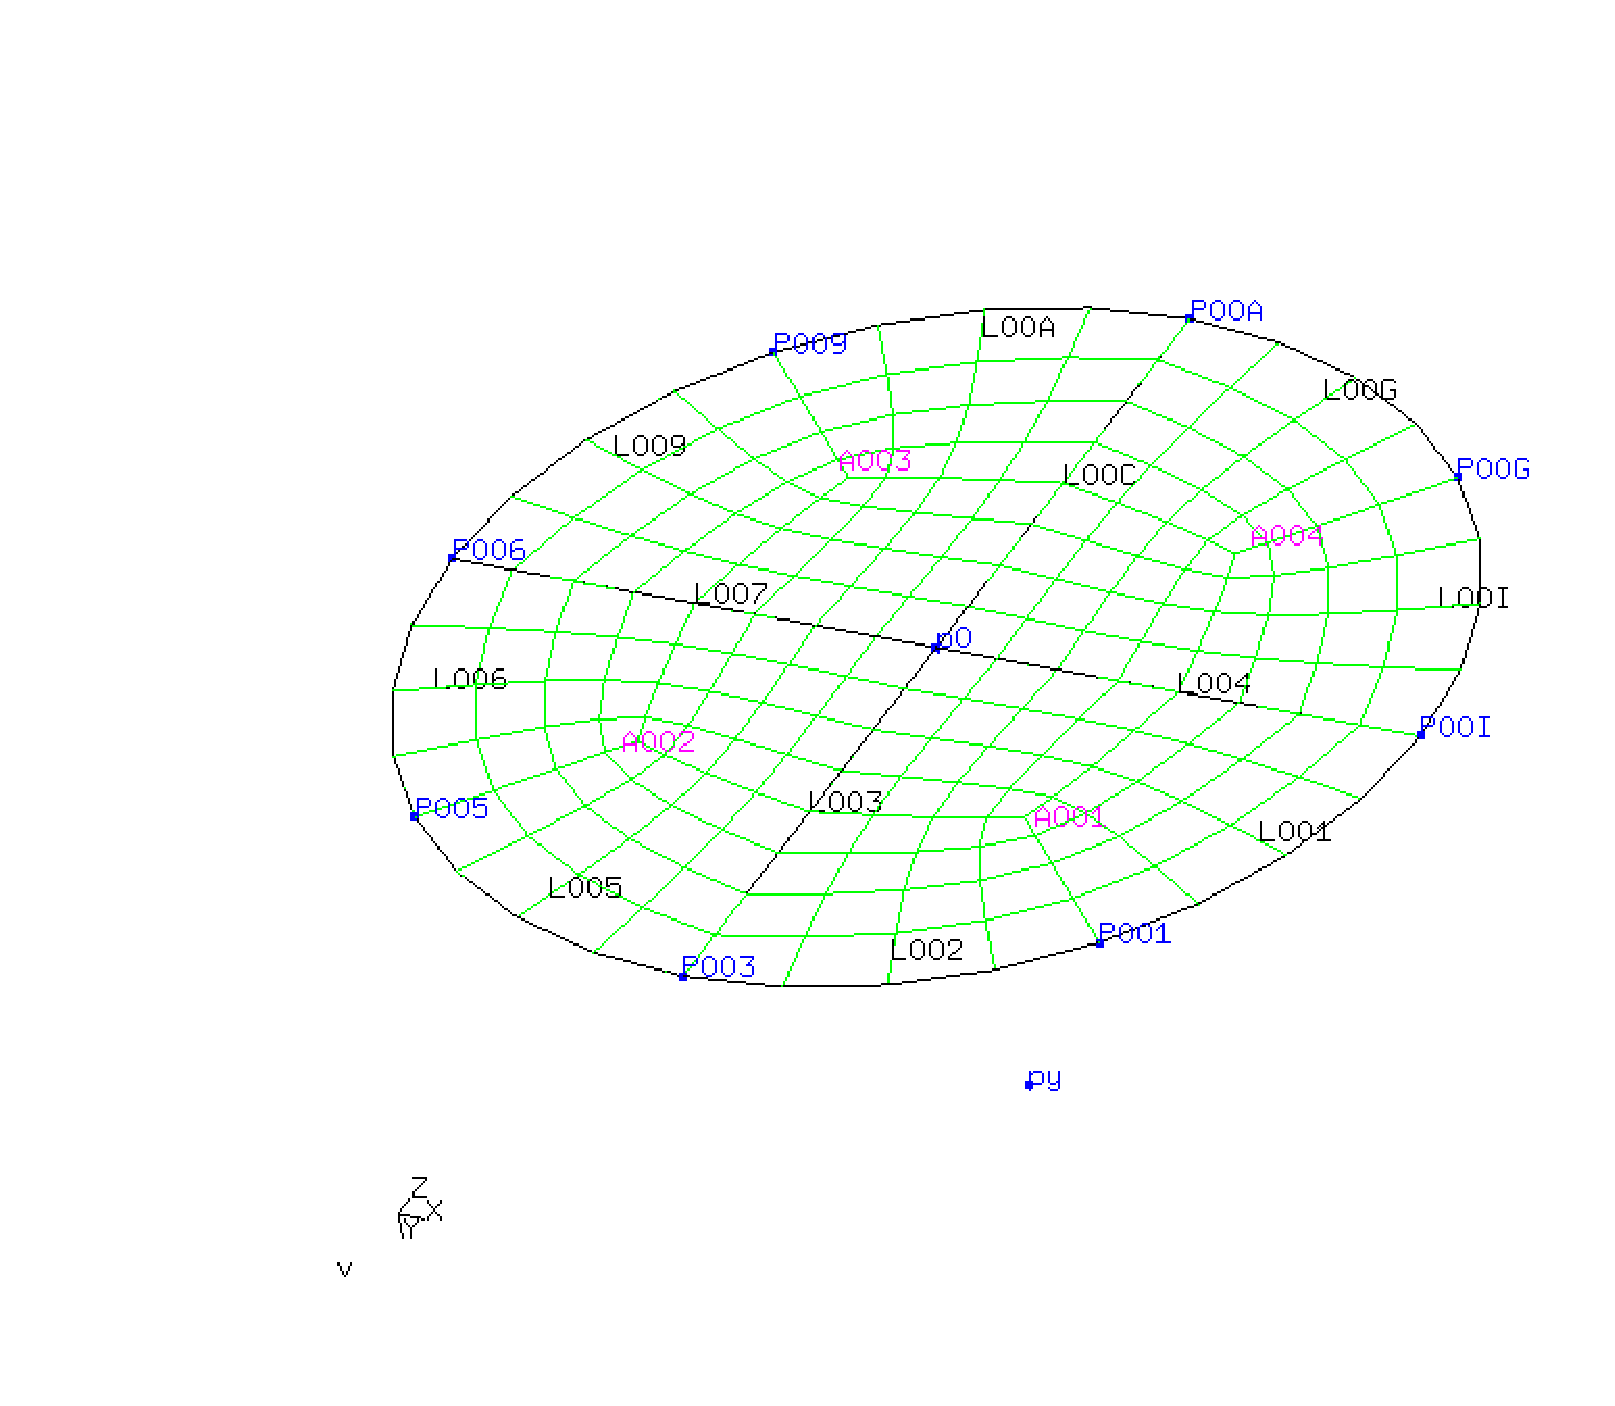
\epsfig{file=disc.eps,width=12cm}
\caption{\label{disc made of four 90 degree segments}disc made of four 90 degree segments}
\end{figure}
\begin{verbatim}
 PNT py      -0.00000        1.00000        0.00000 
 PNT p0      -0.00000       -0.00000        0.00000 
 PNT P001     0.70711       -0.00000       -0.70711 
 PNT P003    -0.00000       -0.00000       -1.00000 
 PNT P005    -0.70711       -0.00000       -0.70711 
 PNT P006    -1.00000       -0.00000        0.00000 
 PNT P009    -0.70711       -0.00000        0.70711 
 PNT P00A     0.00000       -0.00000        1.00000 
 PNT P00G     0.70711       -0.00000        0.70711 
 PNT P00I     1.00000       -0.00000       -0.00000 
 LINE L001 P00I P001 p0 4              
 LINE L002 P001 P003 p0 4              
 LINE L003 P003 p0 8              
 LINE L004 p0 P00I 8              
 LINE L005 P003 P005 p0 4              
 LINE L006 P005 P006 p0 4              
 LINE L007 P006 p0 8              
 LINE L009 P006 P009 p0 4              
 LINE L00A P009 P00A p0 4              
 LINE L00C P00A p0 8              
 LINE L00G P00A P00G p0 4              
 LINE L00I P00G P00I p0 4              
 GSUR A001 + BLEND  - L003 - L002 - L001 - L004 
 GSUR A002 + BLEND  - L007 - L006 - L005 + L003 
 GSUR A003 + BLEND  - L00C - L00A - L009 + L007 
 GSUR A004 + BLEND  + L004 - L00I - L00G + L00C 
 ELTY all QU4 
\end{verbatim}

\subsection{\label{Cylinder}Cylinder}
\begin{figure}[h]
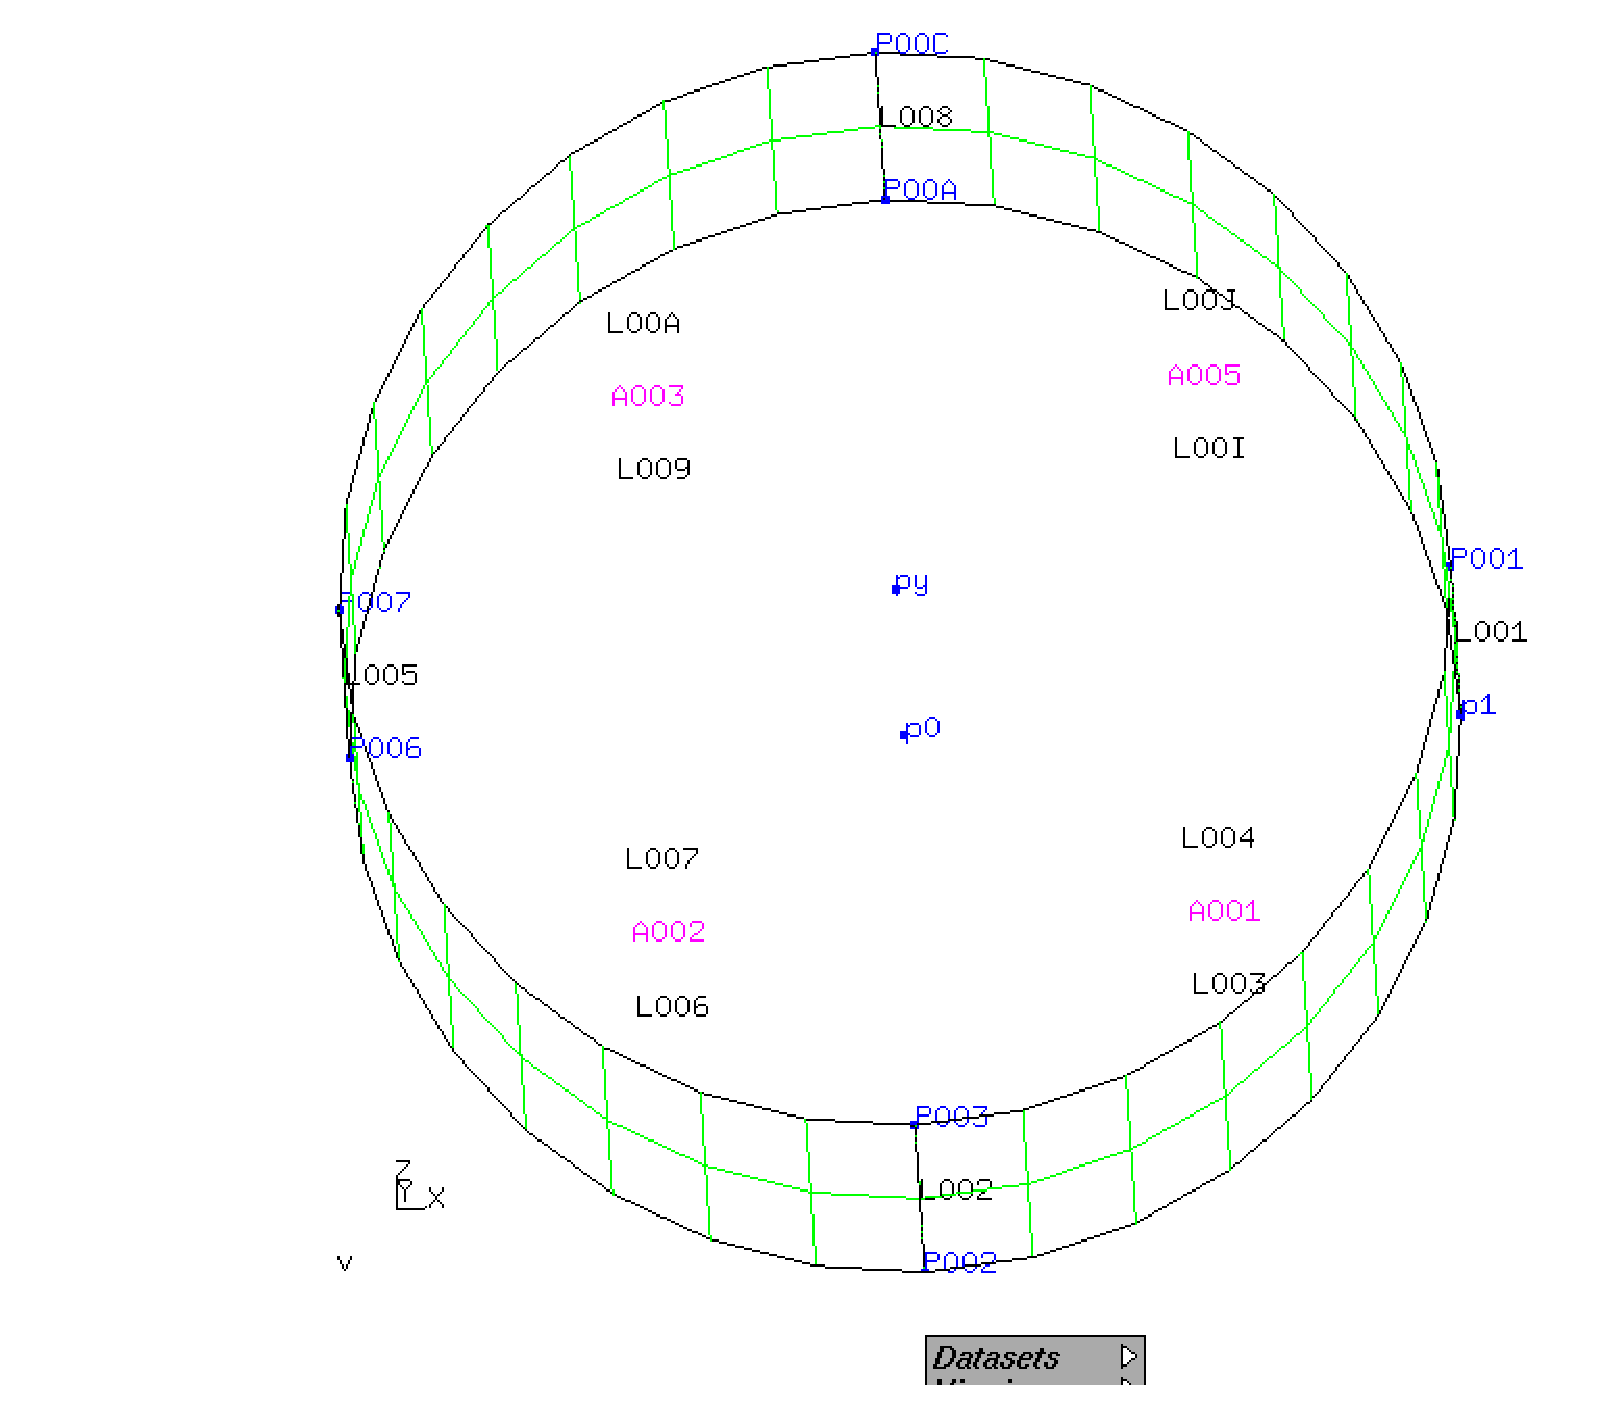
\epsfig{file=cylinder.eps,width=12cm}
\caption{\label{cylinder made of four 90 degree segments}cylinder made of four 90 degree segments}
\end{figure}
\begin{verbatim}
 PNT p0      -0.00000       -0.00000        0.00000 
 PNT py      -0.00000        1.00000        0.00000 
 PNT p1       1.00000       -0.00000        0.00000 
 PNT P001     1.00000        1.00000        0.00000 
 PNT P002    -0.00000       -0.00000       -1.00000 
 PNT P003    -0.00000        1.00000       -1.00000 
 PNT P006    -1.00000       -0.00000        0.00000 
 PNT P007    -1.00000        1.00000        0.00000 
 PNT P00A     0.00000       -0.00000        1.00000 
 PNT P00C     0.00000        1.00000        1.00000 
 LINE L001 p1 P001 2              
 LINE L002 P002 P003 2              
 LINE L003 p1 P002 p0 8              
 LINE L004 P001 P003 py 8              
 LINE L005 P006 P007 2              
 LINE L006 P002 P006 p0 8              
 LINE L007 P003 P007 py 8              
 LINE L008 P00A P00C 2              
 LINE L009 P006 P00A p0 8              
 LINE L00A P007 P00C py 8              
 LINE L00I P00A p1 p0 8              
 LINE L00J P00C P001 py 8              
 GSUR A001 + BLEND  - L001 + L003 + L002 - L004 
 GSUR A002 + BLEND  - L002 + L006 + L005 - L007 
 GSUR A003 + BLEND  - L005 + L009 + L008 - L00A 
 GSUR A005 + BLEND  - L008 + L00I + L001 - L00J 
 ELTY all QU4 
\end{verbatim}

\subsection{\label{Sphere}Sphere}
\begin{figure}[h]
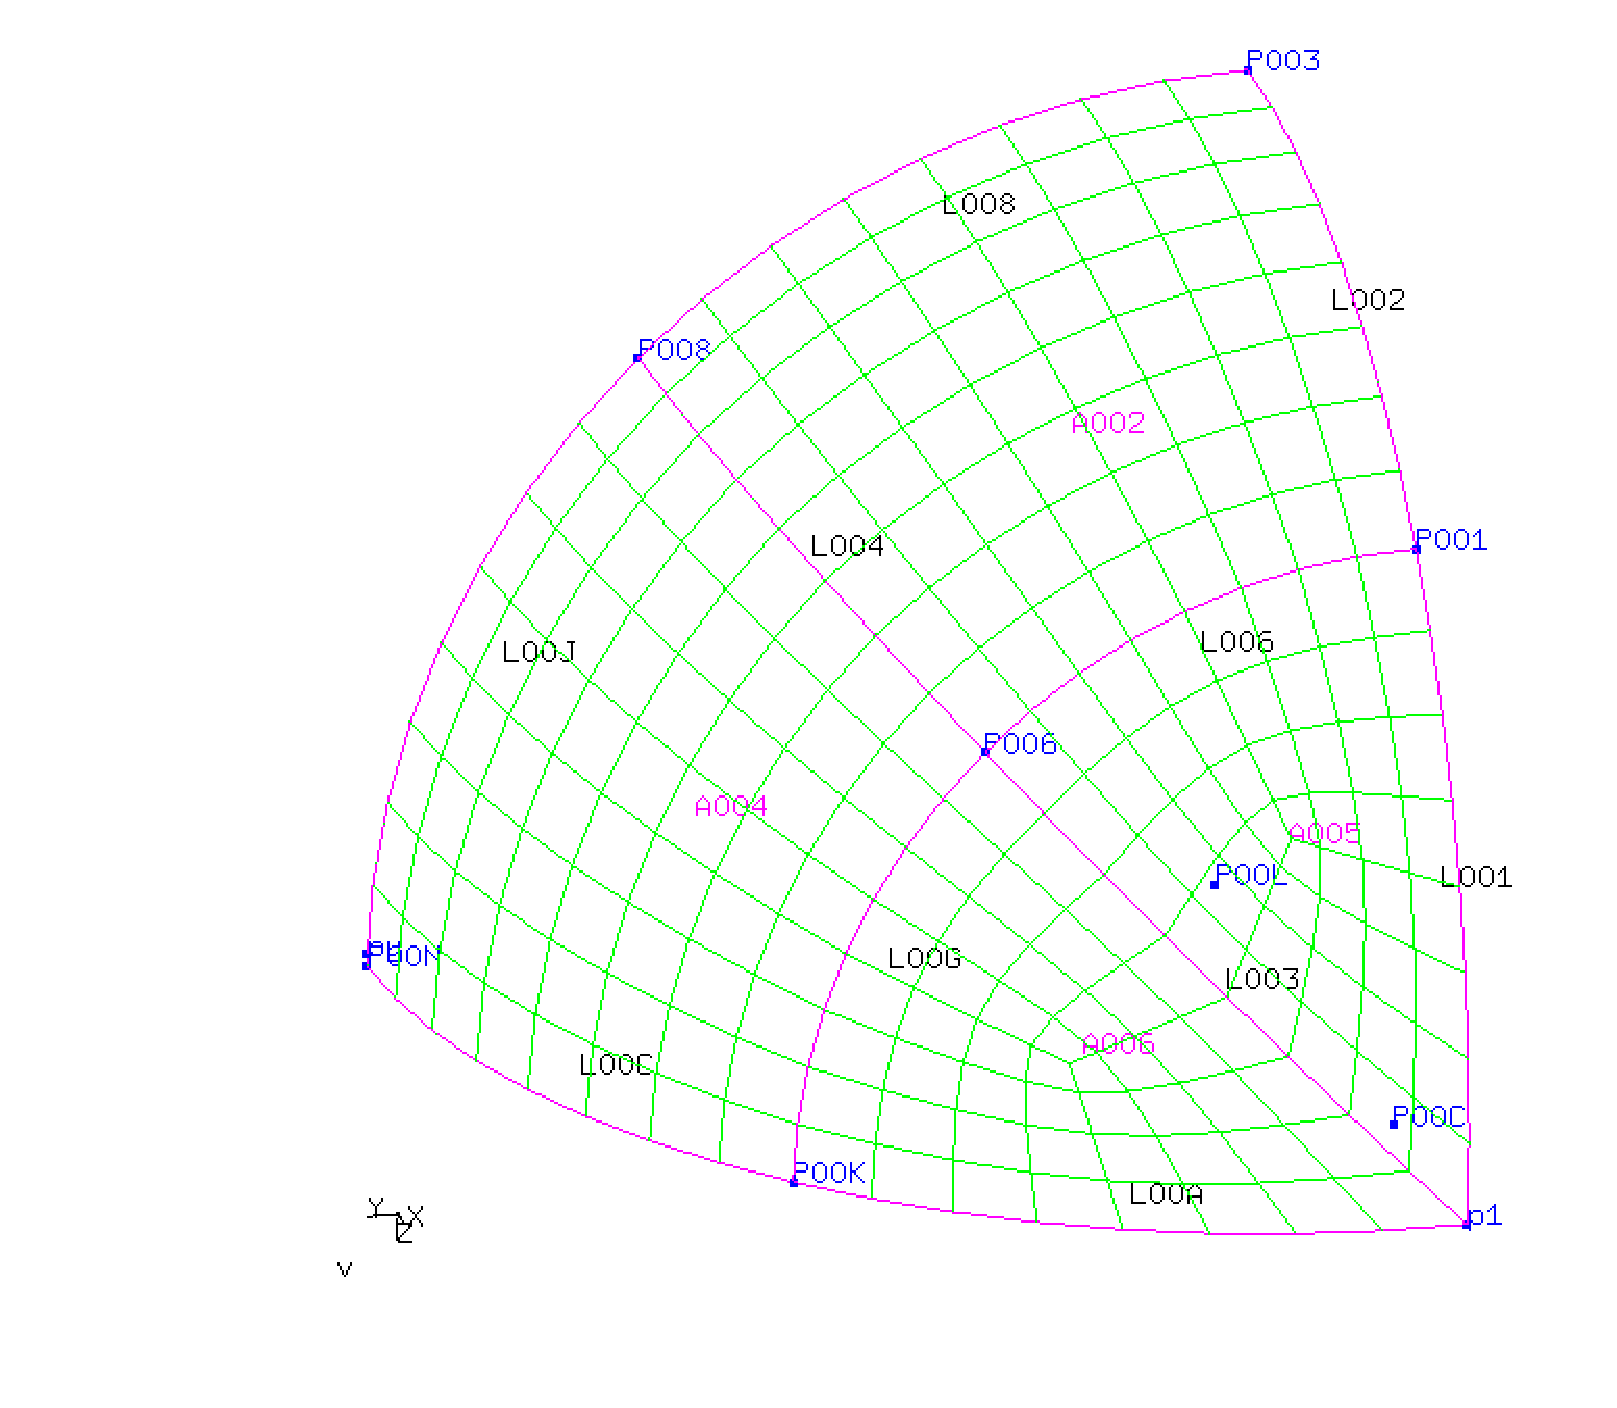
\epsfig{file=sphere.eps,width=12cm}
\caption{\label{Segment of a Sphere}Segment of a Sphere}
\end{figure}
\begin{verbatim}
 PNT py      -0.00000        1.00000       -0.00000 
 PNT p1       1.00000       -0.00000       -0.00000 
 PNT P001     0.70711       -0.00000       -0.70711 
 PNT P003    -0.00000       -0.00000       -1.00000 
 PNT P006     0.70711        0.50000       -0.50000 
 PNT P008    -0.00000        0.70711       -0.70711 
 PNT P00C     0.70711       -0.00000       -0.00000 
 PNT P00K     0.70711        0.70711       -0.00000 
 PNT P00L    -0.00000       -0.00000       -0.00000 
 PNT P00N    -0.00000        1.00000       -0.00000 
 LINE L001 p1 P001 P00L 8              
 LINE L002 P001 P003 P00L 8              
 LINE L003 p1 P006 P00L 8              
 LINE L004 P006 P008 P00L 8              
 LINE L006 P001 P006 P00C 8              
 LINE L008 P003 P008 P00L 8              
 LINE L00A p1 P00K P00L 8              
 LINE L00C P00K P00N P00L 8              
 LINE L00G P006 P00K P00C 8              
 LINE L00J P008 P00N P00L 8              
 GSUR A005 + BLEND  - L003 + L001 + L006 
 GSUR A002 + B\begin{appendix}
LEND  - L002 + L006 + L004 - L008 
 GSUR A006 + BLEND  + L003 + L00G - L00A 
 GSUR A004 + BLEND  - L004 + L00G + L00C - L00J 
 ELTY all QU4 
\end{verbatim}


\subsection{\label{Sphere (Volume)}Sphere (Volume)}
\begin{figure}[h]
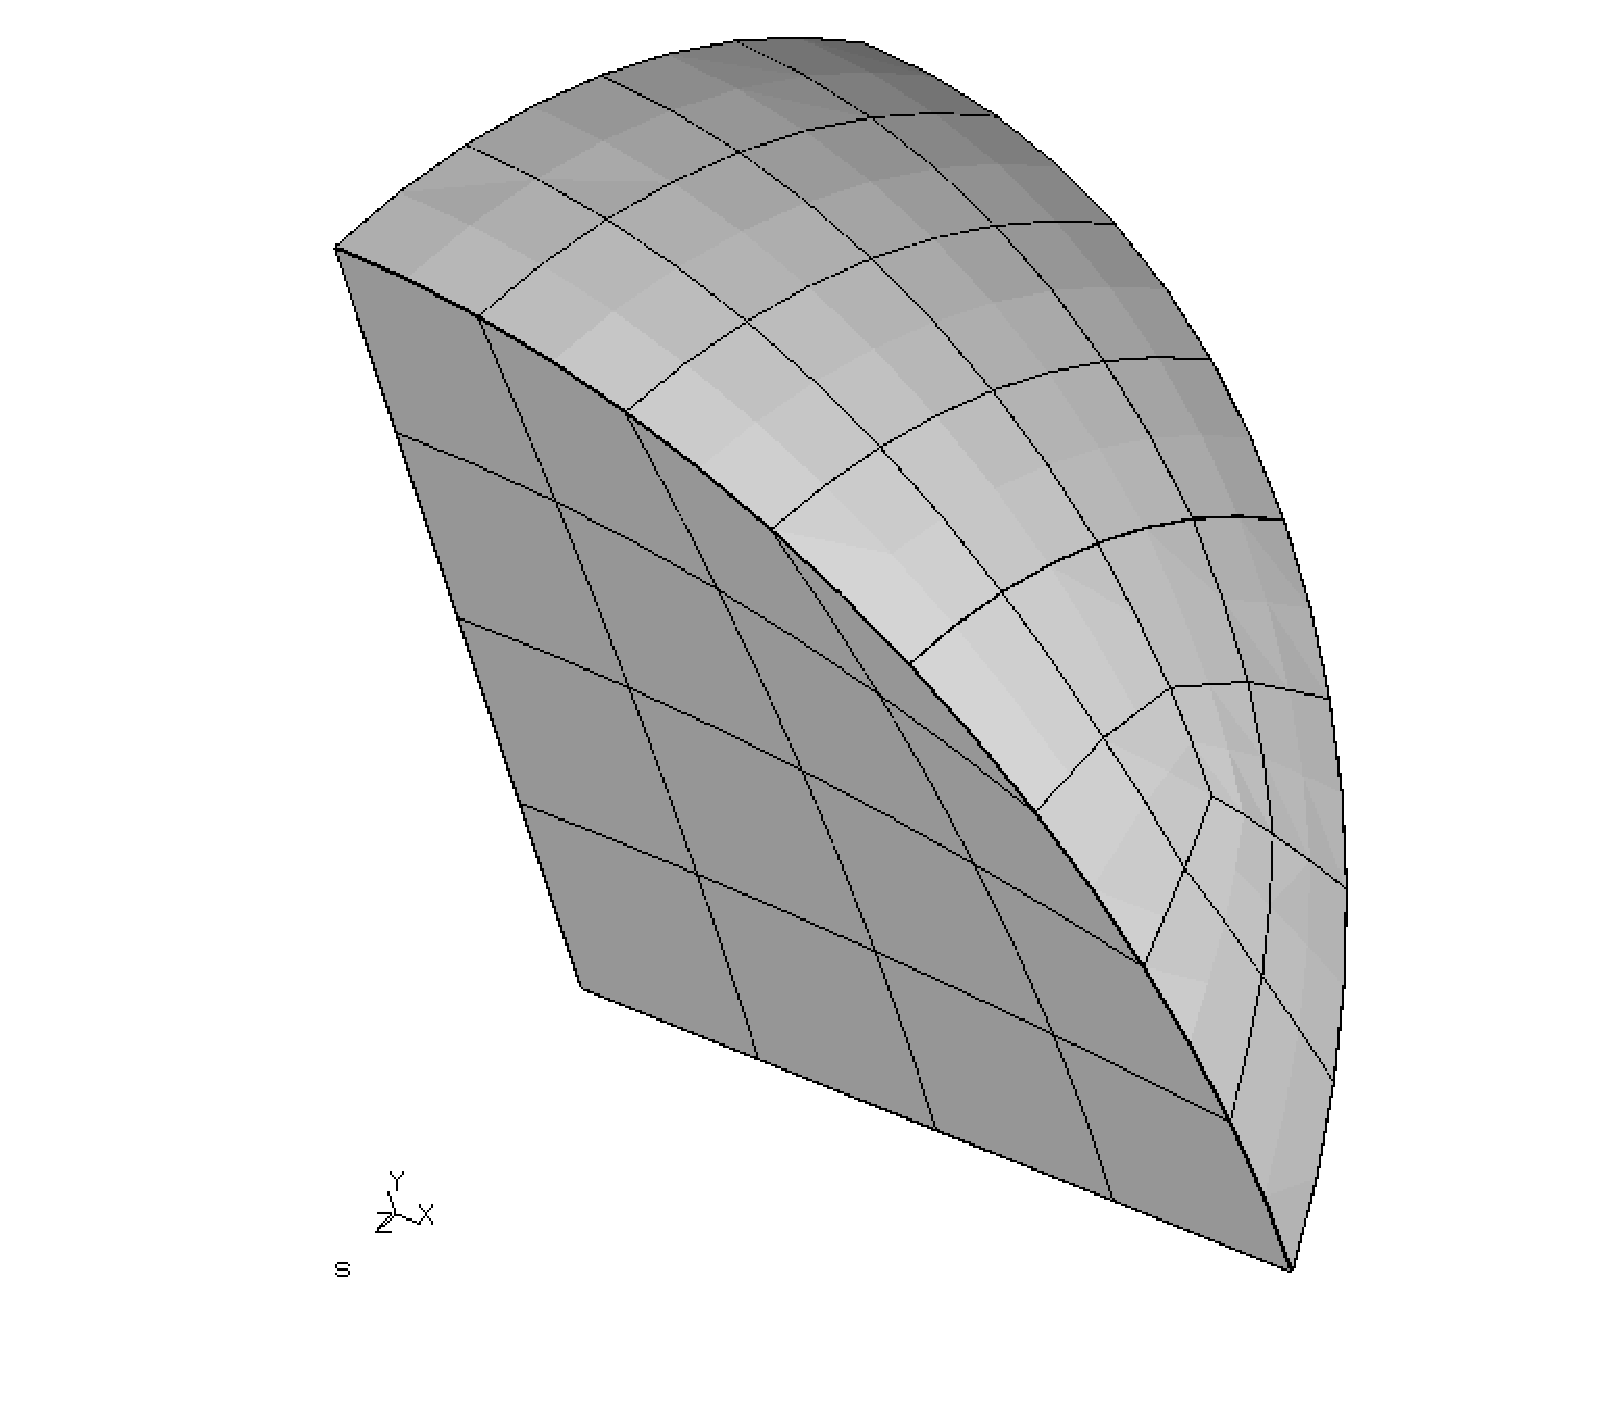
\epsfig{file=sphere_vol.eps,width=12cm}
\caption{\label{Segment of a SphereV}Segment of a Sphere (Volume)}
\end{figure}
\begin{verbatim}
 PNT py       0.00000        1.00000        0.00000 
 PNT p1       1.00000        0.00000        0.00000 
 PNT P006     0.70711        0.50000       -0.50000 
 PNT P008     0.00000        0.70711       -0.70711 
 PNT P00C     0.70711        0.00000        0.00000 
 PNT P00K     0.70711        0.70711        0.00000 
 PNT P00L     0.00000        0.00000        0.00000 
 PNT P00N     0.00000        1.00000        0.00000 
 LINE L001 p1 P00L 8              
 LINE L002 P00L P008 8              
 LINE L003 p1 P006 P00L 8              
 LINE L004 P006 P008 P00L 8              
 LINE L005 P00L P00N 8              
 LINE L00A p1 P00K P00L 8              
 LINE L00C P00K P00N P00L 8              
 LINE L00G P006 P00K P00C 8              
 LINE L00J P008 P00N P00L 8              
 GSUR A001 + BLEND - L003 + L001 + L002 - L004 
 GSUR A002 + BLEND - L005 - L001 + L00A + L00C 
 GSUR A006 + BLEND + L003 + L00G - L00A 
 GSUR A004 + BLEND - L004 + L00G + L00C - L00J 
 GSUR A003 + BLEND + L002 + L00J - L005 
 GBOD B001 NORM + A006 - A003 - A004 + A002 + A001 
 ELTY all HE20 
\end{verbatim}


\subsection{\label{Airfoil for cfd codes}Airfoil for cfd codes}
All surfaces must be oriented in the same way. The sets are used to define areas for the boundary conditions.
\begin{figure}[h]
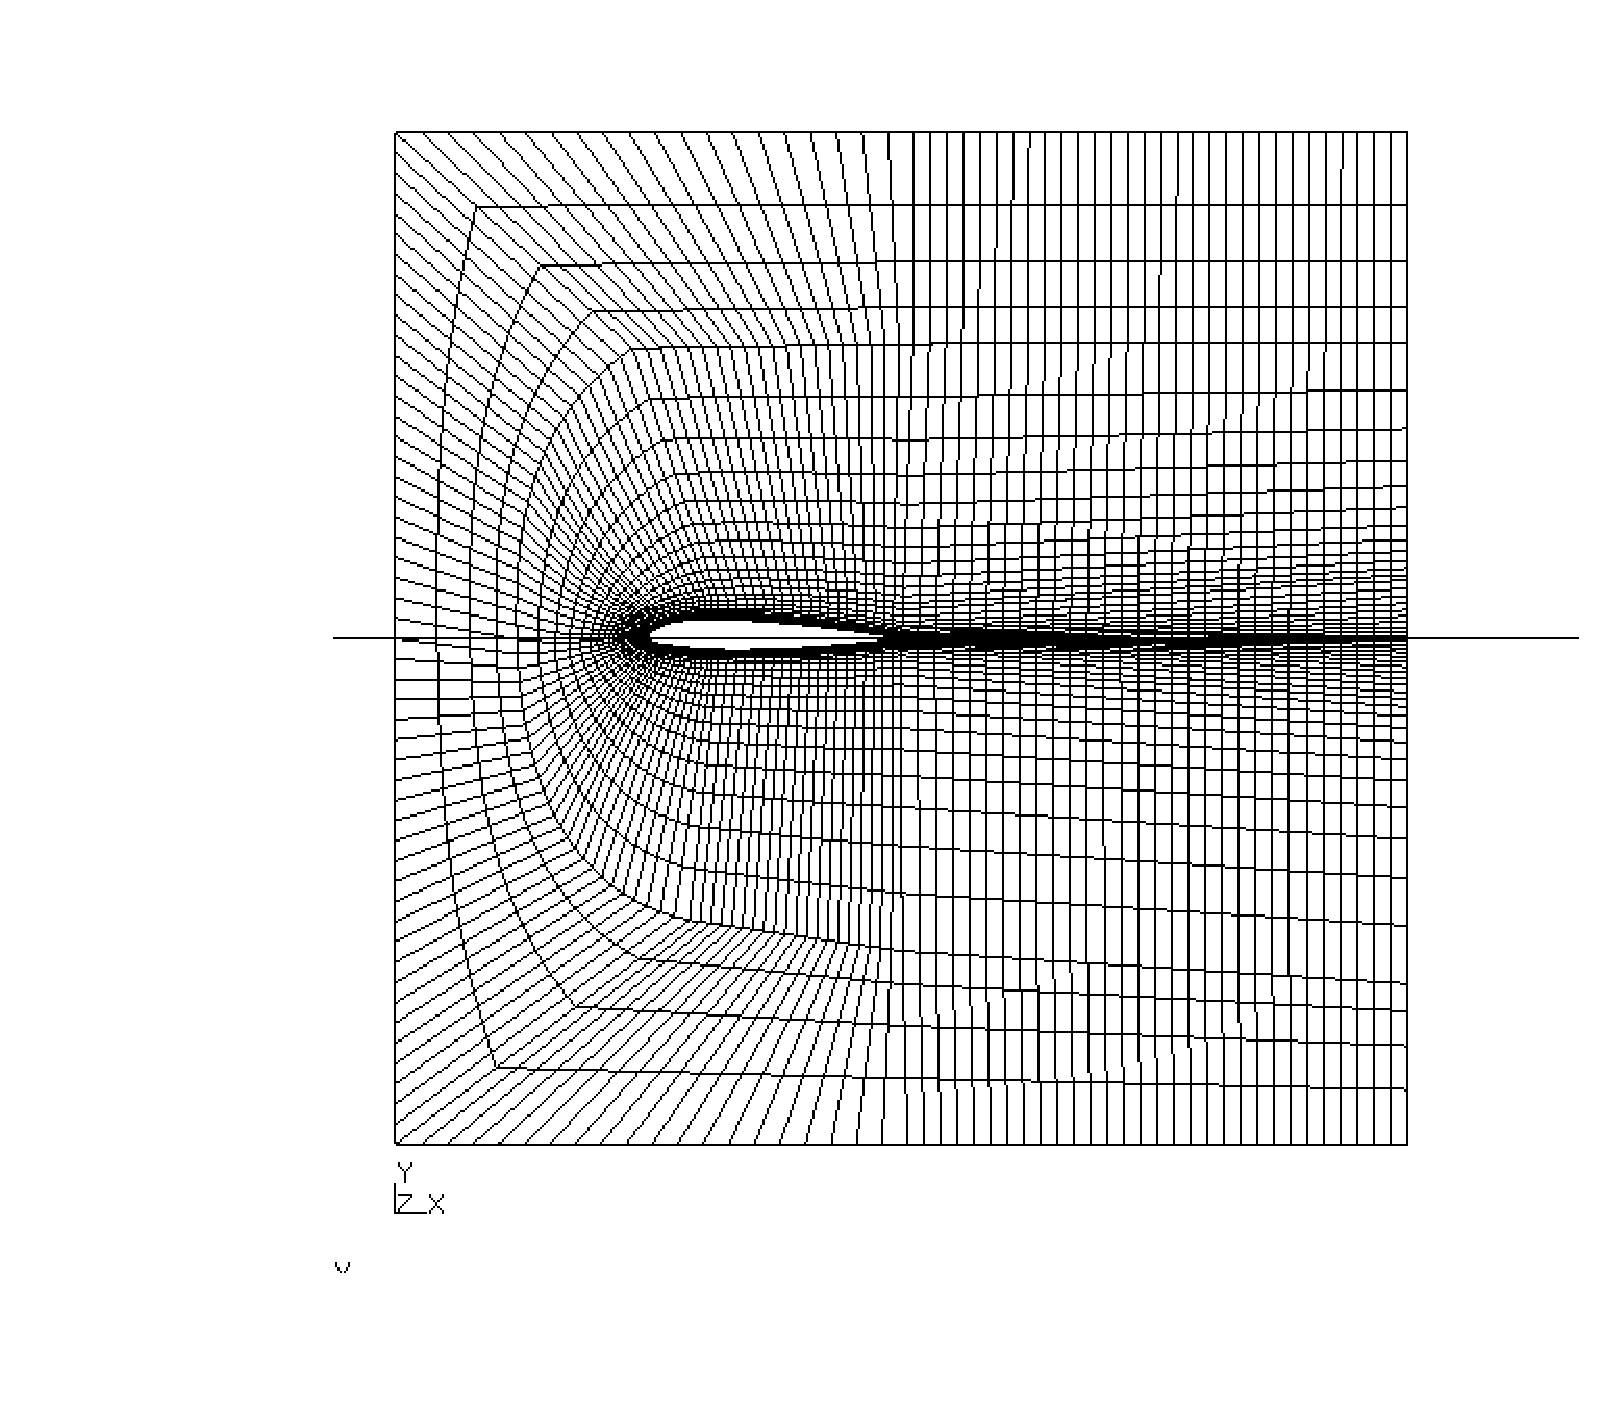
\epsfig{file=naca23012.eps,width=12cm}
\caption{\label{Airfoil for duns}Airfoil for cfd codes }
\end{figure}
\begin{verbatim}
 PNT P002    -0.24688        0.00667        0.00000 
 PNT P003    -0.24375        0.00903        0.00000 
 PNT P004    -0.23750        0.01228        0.00000 
 PNT P005    -0.23125        0.01450        0.00000 
 PNT P006    -0.22500        0.01608        0.00000 
 PNT P007    -0.21250        0.01798        0.00000 
 PNT P008    -0.20000        0.01875        0.00000 
 PNT P009    -0.18750        0.01900        0.00000 
 PNT P00A    -0.17500        0.01888        0.00000 
 PNT P00C    -0.15000        0.01785        0.00000 
 PNT P00E    -0.12500        0.01602        0.00000 
 PNT P00G    -0.10000        0.01368        0.00000 
 PNT P00I    -0.07500        0.01090        0.00000 
 PNT P00J    -0.05000        0.00770        0.00000 
 PNT P00K    -0.02500        0.00420        0.00000 
 PNT P00L    -0.01250        0.00230        0.00000 
 PNT P00O    -0.25000        0.00000        0.00000 
 PNT P00P    -0.24688       -0.00308        0.00000 
 PNT P00R    -0.24375       -0.00427        0.00000 
 PNT P00S    -0.23750       -0.00565        0.00000 
 PNT P00T    -0.23125       -0.00653        0.00000 
 PNT P00V    -0.22500       -0.00730        0.00000 
 PNT P00W    -0.21250       -0.00875        0.00000 
 PNT P00X    -0.20000       -0.00993        0.00000 
 PNT P00Z    -0.18750       -0.01070        0.00000 
 PNT P010    -0.17500       -0.01115        0.00000 
 PNT P011    -0.15000       -0.01120        0.00000 
 PNT P012    -0.12500       -0.01043        0.00000 
 PNT P013    -0.10000       -0.00917        0.00000 
 PNT P014    -0.07500       -0.00750        0.00000 
 PNT P015    -0.05000       -0.00540        0.00000 
 PNT P016    -0.02500       -0.00308        0.00000 
 PNT P017    -0.01250       -0.00175        0.00000 
 PNT P019     0.00000        0.00000        0.00000 
 PNT P1      -0.50000       -0.50000        0.00000 
 PNT P2       0.50000       -0.50000        0.00000 
 PNT p3       0.50000        0.50000        0.00000 
 PNT p4      -0.50000        0.50000        0.00000 
 PNT P01A    -0.18162        0.01898        0.00000 
 PNT P01B    -0.18180       -0.01094        0.00000 
 PNT P046    -0.27025        0.01256        0.00000 
 PNT P059    -0.26599        0.28688        0.00000 
 PNT P049    -0.25144        0.02439        0.00000 
 PNT P05A    -0.35589        0.17566        0.00000 
 PNT P04C    -0.22636        0.03241        0.00000 
 PNT P04D    -0.20128        0.03643        0.00000 
 PNT P05C    -0.38027        0.00958        0.00000 
 PNT P04G    -0.12604        0.03833        0.00000 
 PNT P04H    -0.07588        0.03616        0.00000 
 PNT P04I    -0.02572        0.03231        0.00000 
 PNT P05D    -0.31932       -0.21136        0.00000 
 PNT P04L    -0.27652       -0.00154        0.00000 
 PNT P04M    -0.27025       -0.00803        0.00000 
 PNT P05F    -0.20962       -0.27840        0.00000 
 PNT P04P    -0.25373       -0.01567        0.00000 
 PNT P04R    -0.22676       -0.02143        0.00000 
 PNT P04T    -0.20124       -0.02394        0.00000 
 PNT P05G     0.01132        0.29145        0.00000 
 PNT P04W    -0.12604       -0.02508        0.00000 
 PNT P04X    -0.07588       -0.02519        0.00000 
 PNT P04Z    -0.02572       -0.02355        0.00000 
 PNT P05H     0.00065       -0.30887        0.00000 
 PNT P052    -0.18074        0.03754        0.00000 
 PNT P054    -0.18133       -0.02465        0.00000 
 PNT P056     0.00118        0.02891        0.00000 
 PNT P058     0.00010       -0.02250        0.00000 
 PNT P05I     0.01244        0.50000        0.00000 
 PNT P05J     0.00610       -0.50000        0.00000 
 PNT P05L     0.50000       -0.34112        0.00000 
 PNT P05M     0.50000        0.29206        0.00000 
 PNT P05N     0.50000        0.05780        0.00000 
 PNT P05S     0.50000       -0.05314        0.00000 
 PNT P05V     0.50000       -0.00217        0.00000 
 PNT P00N    -0.23448        0.01345        0.00000 
 PNT P02M    -0.23471       -0.00608        0.00000 
 PNT P03B    -0.24164        0.02804        0.00000 
 PNT P03C    -0.23405       -0.02029        0.00000 
 PNT P03E    -0.24536        0.00794        0.00000 
 PNT P03P    -0.24464       -0.00400        0.00000 
 PNT pl1     -1.00000        0.00000        0.00000 
 PNT pl2      1.00000        0.00000        0.00000 
 SEQA S006  pnt  P01A P00A P00C P00E P00G P00I P00J P00K P00L P019
 SEQA S007  pnt  P019 P017 P016 P015 P014 P013 P012 P011 P010 P01B
 SEQA S00W  pnt  P03B P049 P046 P04L P04M P04P P03C
 SEQA S00R  pnt  P052 P04G P04H P04I P056
 SEQA S00S  pnt  P058 P04Z P04X P04W P054
 SEQA S00T  pnt  P05F P05D P05C P05A P059
 SEQA S001  pnt  P01A P009 P008 P007 P006 P005 P00N
 SEQA S00E  pnt  P03E P002 P00O P00P P03P
 SEQA S00L  pnt  P052 P04D P04C P03B
 SEQA S00A  pnt  P02M P00T P00V P00W P00X P00Z P01B
 SEQA S00X  pnt  P03C P04R P04T P054
 SEQA S002  pnt  P00N P004 P003 P03E
 SEQA S00P  pnt  P03P P00R P00S P02M
 LINE L003 P01A P052 910
 LINE L00C P01A P019 S006 120
 LINE L00E P019 P01B S007 120
 LINE L004 p4 P1 150
 LINE L05F P2 P05L -204
 LINE L05S P05L P05S -912
 LINE L05C P1 P05J 120
 LINE L006 P01B P054 910
 LINE L007 P019 P056 910
 LINE L008 P058 P019 -910
 LINE L00G P05S P05V -210
 LINE L00N P03B P03C S00W 130
 LINE L03R P052 P056 S00R 120
 LINE L00I P05V P05N 210
 LINE L03S P058 P054 S00S 120
 LINE L04V p4 P059 -204
 LINE L04W P059 P052 -912
 LINE L04X P054 P05F 912
 LINE L04Z P05F P1 204
 LINE L050 P05F P059 S00T 150
 LINE L052 P059 P05G 120
 LINE L054 P05F P05H 120
 LINE L056 P05H P058 -912
 LINE L058 P056 P05G 912
 LINE L059 p3 P05I 130
 LINE L05A P05I p4 120
 LINE L05D P05J P2 130
 LINE L05V P056 P05N 130
 LINE L05I P05M p3 204
 LINE L05L P05N P05M 912
 LINE L05Z P058 P05S 130
 LINE L06C P019 P05V 130
 LINE L06F P05M P05G 130
 LINE L06H P05G P05I 204
 LINE L06I P05L P05H 130
 LINE L06J P05H P05J 204
 LINE L001 P01A P00N S001 -210
 LINE L00A P03E P03P S00E 120
 LINE L00K P052 P03B S00L 110
 LINE L009 P02M P01B S00A 210
 LINE L00O P03C P054 S00X 110
 LINE L002 P00N P03E S002 -205
 LINE L00L P03P P02M S00P 205
 LINE cl pl1 pl2 120
 LINE L005 P00O P019 120
 LCMB C001  + L001 + L002 + L00A + L00L + L009 
 LCMB C004  + L00K + L00N + L00O 
 GSUR A001 + BLEND + L003 + C004 - L006 - C001 
 GSUR A002 + BLEND + L006 - L03S + L008 + L00E 
 GSUR A003 + BLEND + L00C + L007 - L03R - L003 
 GSUR A004 + BLEND - L008 + L05Z + L00G - L06C 
 GSUR A005 + BLEND + L06C + L00I - L05V - L007 
 GSUR A00I + BLEND - L04W - L050 - L04X - C004 
 GSUR A00J + BLEND - L04V + L004 - L04Z + L050 
 GSUR A00K + BLEND + L04Z + L05C - L06J - L054 
 GSUR A00L + BLEND + L06J + L05D + L05F + L06I 
 GSUR A00N + BLEND + L04V + L052 + L06H + L05A 
 GSUR A00O + BLEND - L06H - L06F + L05I + L059 
 GSUR A00P + BLEND + L04W + L03R + L058 - L052 
 GSUR A00R + BLEND + L04X + L054 + L056 + L03S 
 GSUR A00S + BLEND - L058 + L05V + L05L + L06F 
 GSUR A00T + BLEND - L056 - L06I + L05S - L05Z 
 SETA wall l L05C 
 SETA wall l L059 
 SETA wall l L05A 
 SETA wall l L05D 
 SETA profil l L00C 
 SETA profil l L00E 
 SETA profil l L001 
 SETA profil l L00A 
 SETA profil l L009 
 SETA profil l L002 
 SETA profil l L00L 
 SETA in l L004 
 SETA out l L05F 
 SETA out l L05S 
 SETA out l L00G 
 SETA out l L00I 
 SETA out l L05I 
 SETA out l L05L 
\end{verbatim}


\subsection{\label{If and while demo}If and while demo}
\begin{figure}[h]
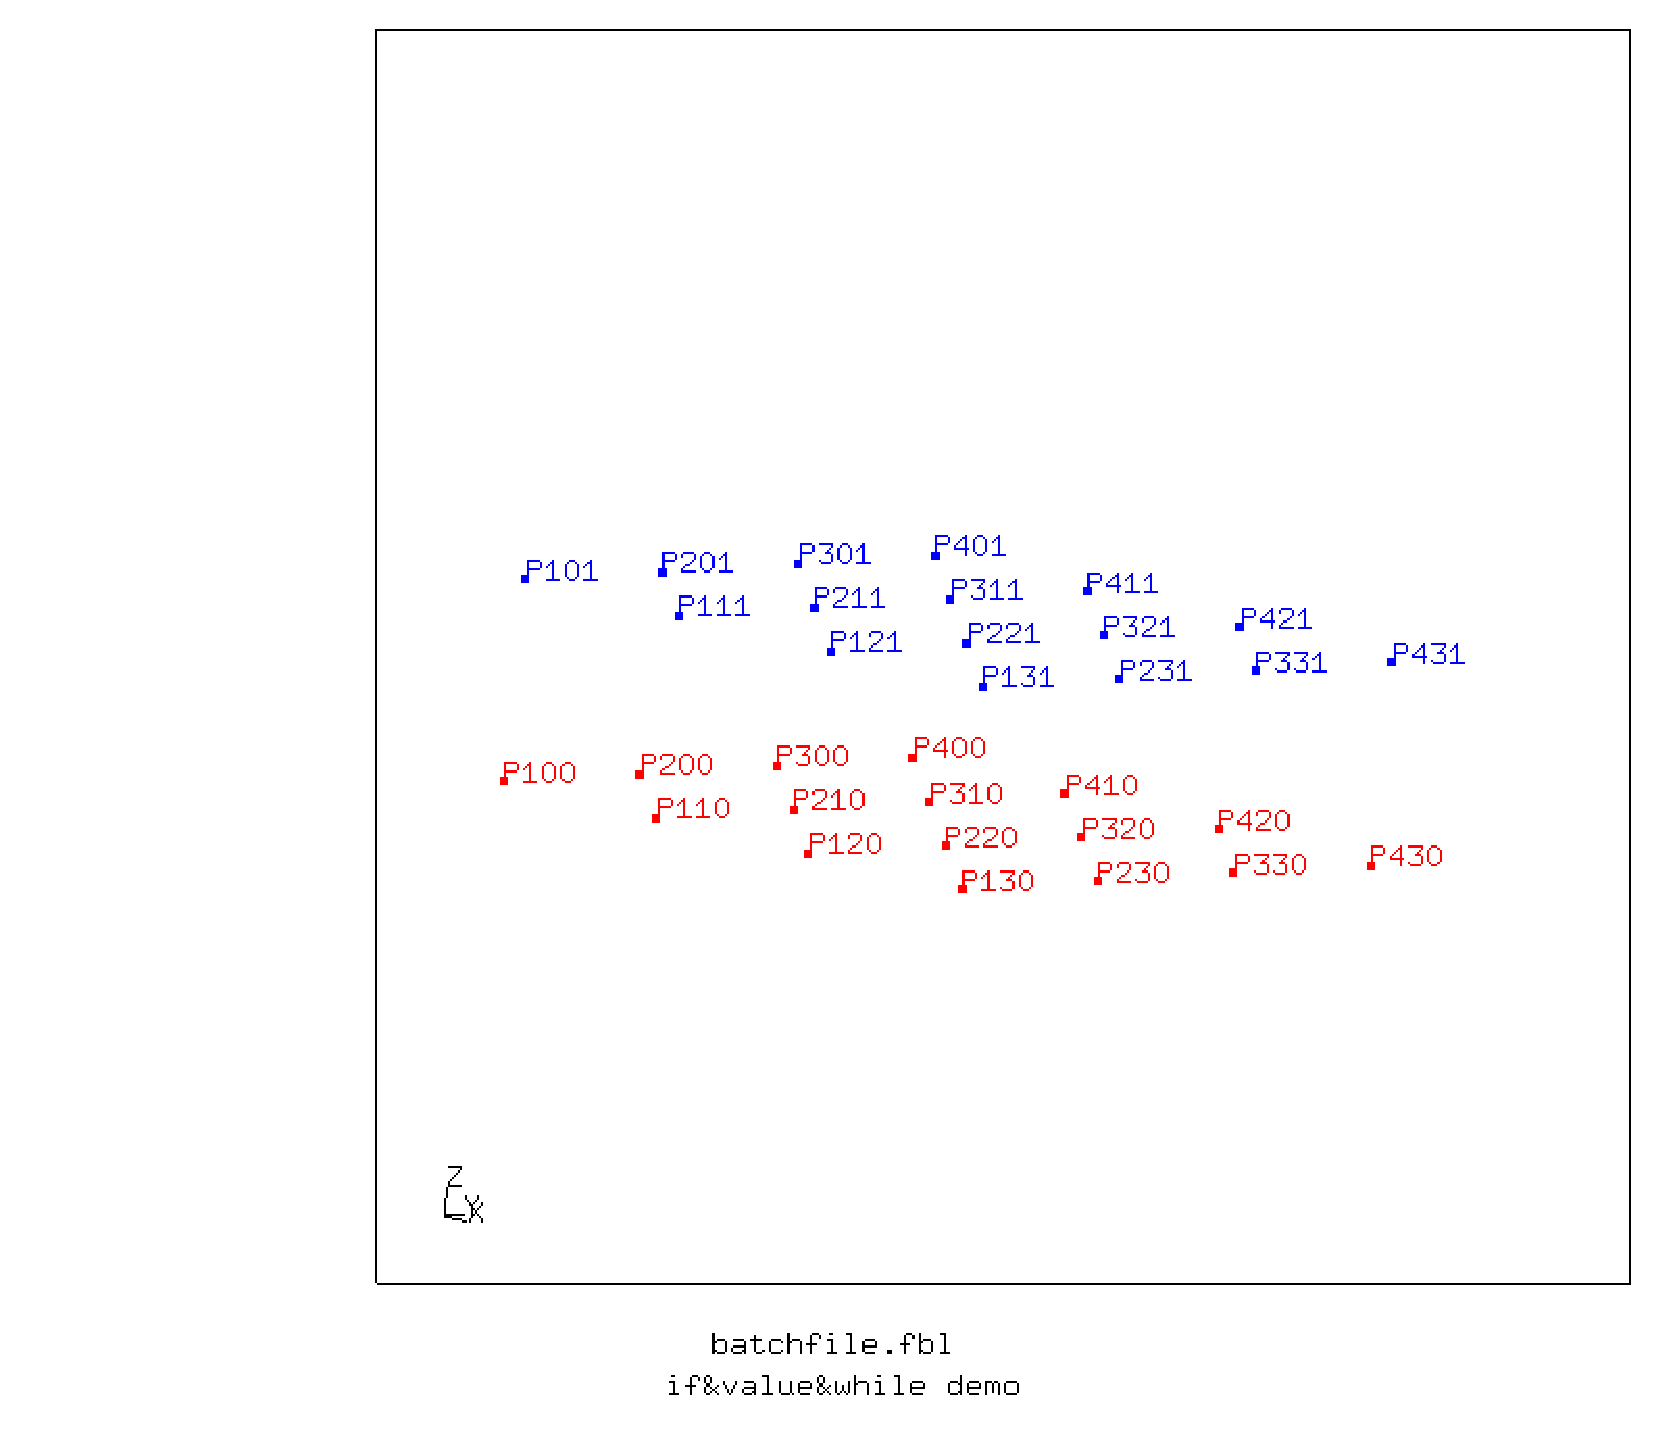
\epsfig{file=ifwhile.eps,width=12cm}
\caption{\label{Result of If and while demo}Result of If and while demo}
\end{figure}
The if and while commands can be nested. A demo which produces some points on the window follows:
\begin{verbatim}
text if&value&while demo
# def the leading letter of point names
valu vp P
# define the initial x value
valu vx 0.
# define parameters
valu v2 4
valu v3 1
# start loop:
while vx < v2
 valu vy 0.
 valu vz 0.
 seto S1
 while vy < v2
  # define the pnt coordinates
  valu vy + vy v3
  valu vy int vy
  valu vx int vx
  valu vz int vz
  # define the pnt name
  valu p1 & vp vy
  valu p1 & p1 vx
  valu p1 & p1 vz
  # generate the pnt
  pnt p1 vx vy vz
 endwhile
 setc
 valu vy 0.
 valu vz 1.
 seto S2
 while vy < v2
  valu vy + vy v3
  valu vy int vy
  valu vx int vx
  valu vz int vz
  valu p2 & vp vy
  valu p2 & p2 vx
  valu p2 & p2 vz
  pnt p2 vx vy vz
 endwhile
 setc
 valu vx + vx v3
 if vx == 1
   plot pa S1 r
 else
   plus pa S2 b
 endif
endwhile
send all fbd
# demo on how to write the content of variables to writedemo.txt
valu vx int vx
valu vy int vy
sys echo VX: vx VY: vx VZ: vz >| writedemo.txt
\end{verbatim}

\end{appendix}

\begin{thebibliography}{99}

\bibitem{mesa} OpenGL-Like Rendering Toolkit, from Brian Paul, http://www.mesa3d.org/ 

\bibitem{glut} OpenGL Utility Toolkit (GLUT), from Mark J. Kilgard
%, http://reality.sgi.com/mjk_asd/glut3/glut3.html, Copying-Policy: Freely redistributable, not public domain.

\bibitem{cgx} CalculiX GraphiX (cgx), from Klaus Wittig, klaus.wittig@calculix.de
\bibitem{NETGEN} NETGEN, unstructured mesher, http://www.hpfem.jku.at/netgen/
\bibitem{dolfyn} dolfyn, Open Source CFD code, http://www.dolfyn.net
\bibitem{duns} Duns, a two- and three dimensional cfd code, http://sourceforge.net/projects/duns/
 \bibitem{isaac} ISAAC, a two- and three dimensional cfd code, http://isaac-cfd.sourceforge.net
\bibitem{OpenFOAM} OpenFOAM, a three dimensional cfd code, http://www.opencfd.co.uk
\bibitem{tochnog} Tochnog, a free fem-code, http://tochnog.sourceforge.net/
\bibitem{tutorial} Tutorial for CalculiX, from Dr. Guido Dhondt, http://www.dhondt.de/tutorial.html

\bibitem{ImageMagick} ImageMagick 5.1.0 00/01/01 Q:8 cristyg@mystic.es.dupont.com. Copyright: Copyright (C) 2000 ImageMagick Studio 

\bibitem{Firefox} Mozilla Foundation, http://www.firefox.com

\bibitem{Coons} S. A. Coons, 'Surfaces for computer-aided design of space forms'. Project MAC, MIT (1964). Revised to MAC-TR-41 (1967). 
\bibitem{mesh2d} mesh2d, unstructured 2D-mesher from B. Kaan Karamete, Ph.D, No URL Available

\bibitem{spline} Paul Dierckx, Curve and Surface Fitting with Splines, Oxford. University Press, 1993

\end{thebibliography}

\end{document}
